
\documentclass[headsepline,footinclude=false,fontsize=11pt,paper=a4,listof=totoc,bibliography=totoc,BCOR=12mm,DIV=14]{scrbook} 

\usepackage[backend=bibtex]{biblatex}
\bibliography{bibliography.bib} 

\usepackage{fancyhdr}
\usepackage{graphicx}
\usepackage{glossaries}
\makeglossaries
\usepackage[linesnumbered,ruled,vlined]{algorithm2e}
\usepackage[urlcolor=blue]{hyperref}

\pagestyle{fancy}
\fancyhf{}
\fancyhead[LE,RO]{\textbf{\thepage}}
\fancyhead[LO]{\rightmark}
\fancyhead[RE]{\leftmark}
\renewcommand{\headrulewidth}{0.5pt}

\setlength\parindent{0pt}
\usepackage{listings}
\parskip 1.5ex 

\linespread{1.15}
\usepackage[scaled]{helvet}
\usepackage[T1]{fontenc}
\renewcommand\familydefault{\sfdefault}


\begin{document}

\newglossaryentry{hmd}{name=HMD, description={Head Mounted Display}}
\newglossaryentry{kst}{name=KST, description={KUKA Sunrise Toolbox}}
\newglossaryentry{ptp}{name=PTP, description={Point to point}}
\newglossaryentry{ros}{name=ROS, description={Robot Operating System}}
\newglossaryentry{rgbd}{name=RGB-D, description={Red-Green-Blue-Depth}}
\newglossaryentry{vr}{name=VR, description={Virtual reality}}
\newglossaryentry{gui}{name=GUI, description={Graphical User Interface}}

\begin{titlepage}
	\centering
	\vspace*{10mm}
	\huge Imperial College London
	\vspace{30mm}
	
	\large \textbf{Mechatronics in Medicine Laboratory}
	
	\vspace{10mm}
	A modular \gls{ros} platform for virtual reality assisted teleoperation of KUKA iiwa robot manipulators and ReFlex TakkTile robotic hand supporting the Leap Motion gesture tracking device
	
	\vspace{10mm}
	Project Report
	
	\vspace{70mm}
	\begin{tabular}{l l}
    Author:          & Alexander Koenig \\
    Supervisors:     & Dr. Fabio Tatti \\
    				 & Dr. Riccardo Secoli \\
    Advisor:         & Prof. Dr. Ferdinando Rodriguez y Baena \\
    Dates: 	 		 & 01.04.2019 - 12.09.2019 \\
    \end{tabular}
	
\end{titlepage}

\printglossaries
\listoffigures{}
\listoftables{}

\tableofcontents

\chapter{Introduction}

In this report a modular \gls{ros} platform for the teleoperation of a KUKA iiwa (7 R800 or 14 R820) robot manipulator and an attached ReFlex TakkTile robotic hand is presented. The system supports the control of both devices using the Leap Motion gesture tracking device. It also features the integration of a depth camera and a virtual reality \gls{hmd}. The following sections give a brief overview of the involved hardware and software components. Since this is a modular system not all pieces of hardware (or software) are needed to run a specific functionality of the system.

\section{Hardware Components}


\begin{figure}[h]
    \centering
    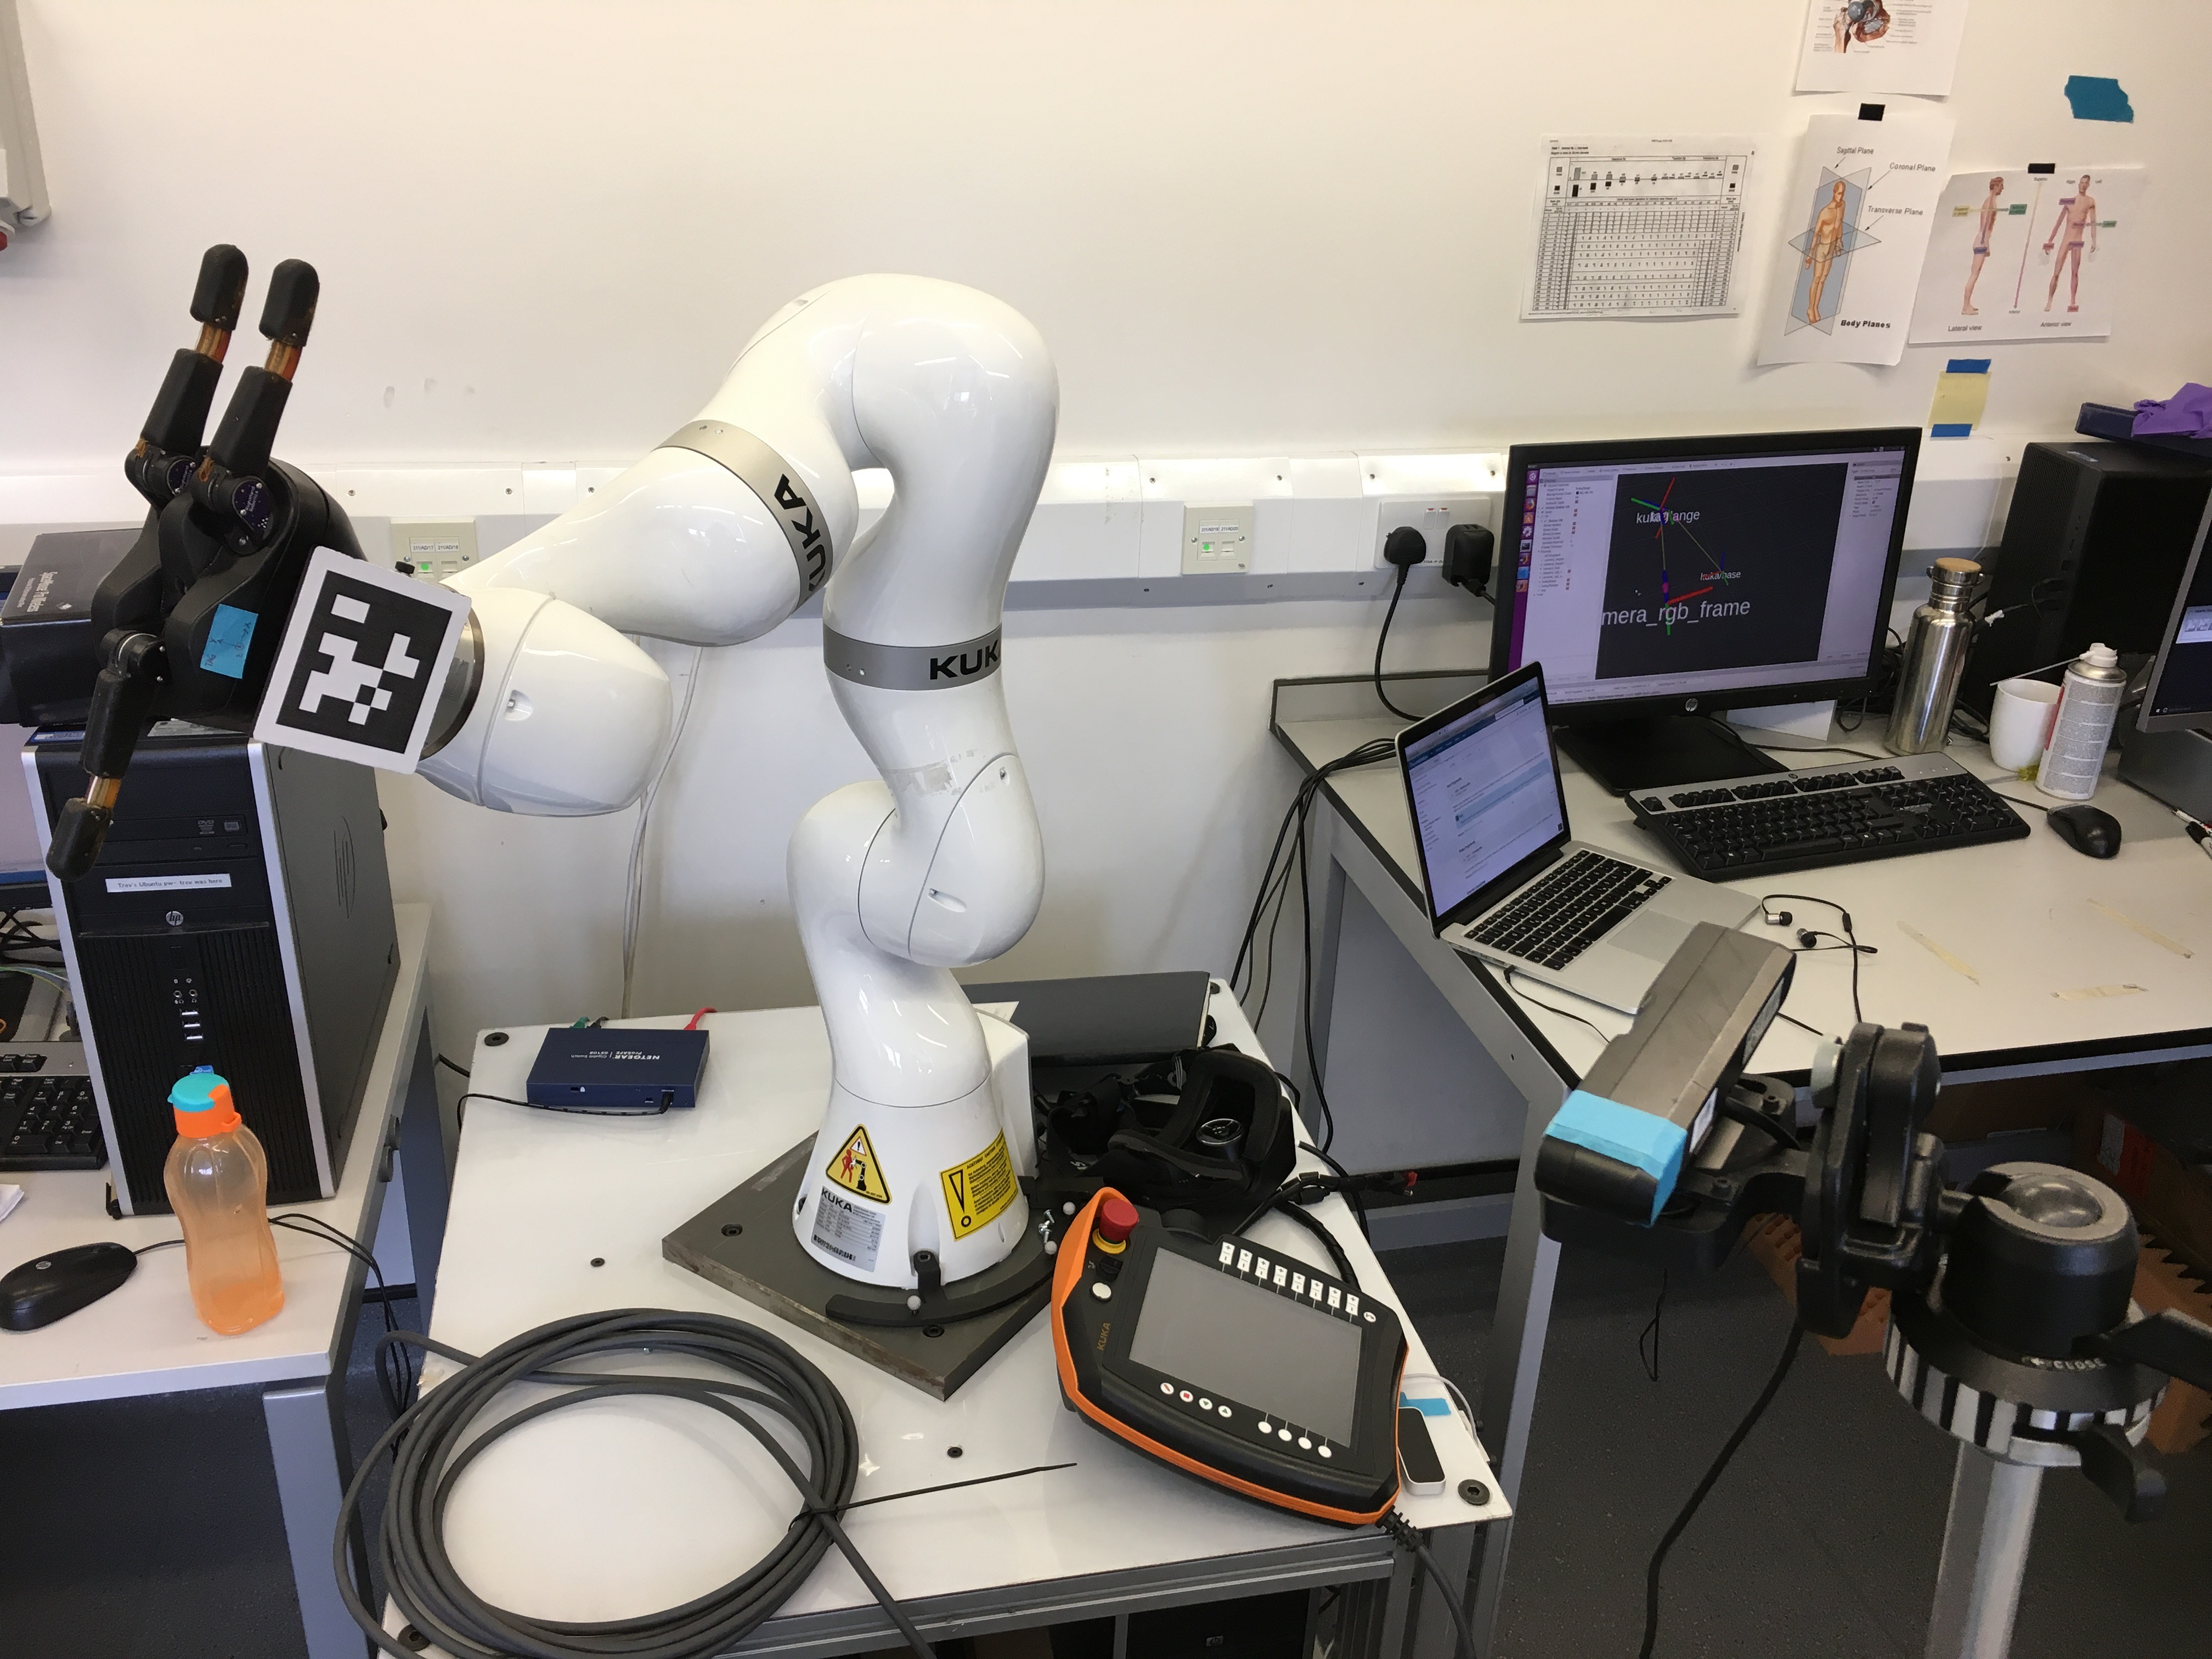
\includegraphics[height=9cm]{images/hardware_overview}
    \caption{Overview of robotic rig}
    \label{fig:hardware_overview}
\end{figure}

Figure \ref{fig:hardware_architecture} shows an overview of the hardware architecture of the robotic rig. Ethernet cables should be category 5 or higher. The \gls{rgbd} camera is mounted on a tripod. 

\newpage
\begin{itemize}
\item
  KUKA iiwa 7 R800 or 14 R820
\item
  ReFlex TakkTile Robotic Hand
\item
  Leap Motion
\item
  Oculus Rift DK2
\item
  Asus Xtion Pro Live
\item
  Switch
\item
  3 ethernet cables
\end{itemize}

\begin{figure}[p]
    \centering
    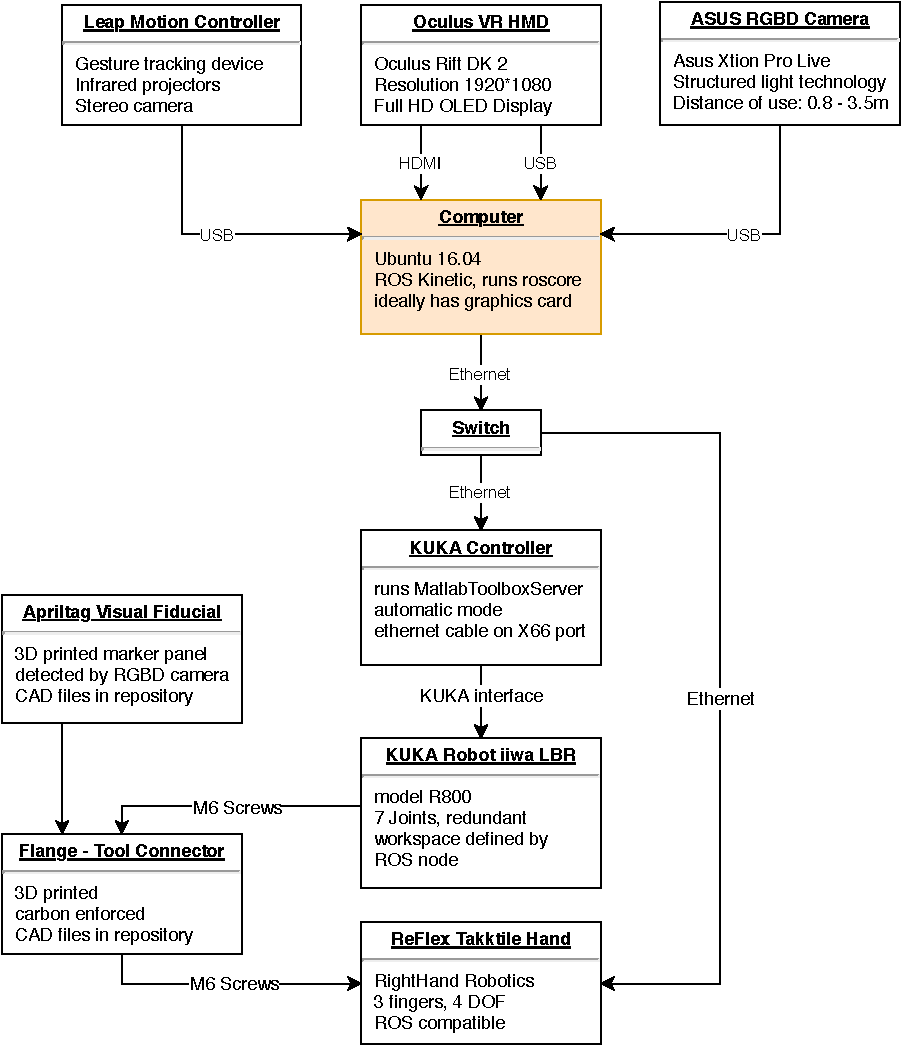
\includegraphics[width=\textwidth]{images/hardware}
    \caption{Hardware architecture}
    \label{fig:hardware_architecture}
\end{figure}

\section{Software Components}

The system was developed and tested using the following software.

\begin{itemize}
\item
  Ubuntu Xenial 16.04 LTS
\item
  Python 2.7
\item
  Numpy 1.11.0
\item
  MATLAB Version 9.6 (R2019a)
\item
  MATLAB Instrument Control Toolbox Version 4.0 (R2019a)
\item
  MATLAB \href{https://uk.mathworks.com/help/robotics/ug/install-robotics-system-toolbox-support-packages.html}{Robotics System Toolbox} Version 2.2 (R2019a)
\item
  MATLAB \href{https://uk.mathworks.com/matlabcentral/fileexchange/49810-robotics-system-toolbox-interface-for-ros-custom-messages}{Robotics System Toolbox Interface for \gls{ros} Custom Messages}
\item
  \href{http://wiki.ros.org/kinetic/Installation/Ubuntu}{ROS Kinetic} (Desktop Install recommended)
\item
  KUKA MatlabToolboxServer on KUKA Robot Controller. See user guide of \href{https://github.com/Modi1987/KST-Kuka-Sunrise-Toolbox}{KUKA Sunrise Toolbox}
\item
  Only for grasp prediction: CUDA V10.1.168 (currently not needed)
\item
  Only for grasp prediction: Conda 4.6.14 (installed miniconda2)
\item
  Only for grasp prediction: Conda environment with dependencies in grasping/env/environment.yaml
\end{itemize}


Figure \ref{fig:software_architecture} shows an overview of the \gls{ros} network used for the control of the robotic rig using the Leap Motion tracking device. The \gls{ros} nodes for the integration of the \gls{vr} display and the depth camera into the platform are intentionally not displayed in Figure \ref{fig:software_architecture} since these nodes run completely independently from the control of the robotic rig using the Leap Motion.

\begin{figure}[p]
    \centering
    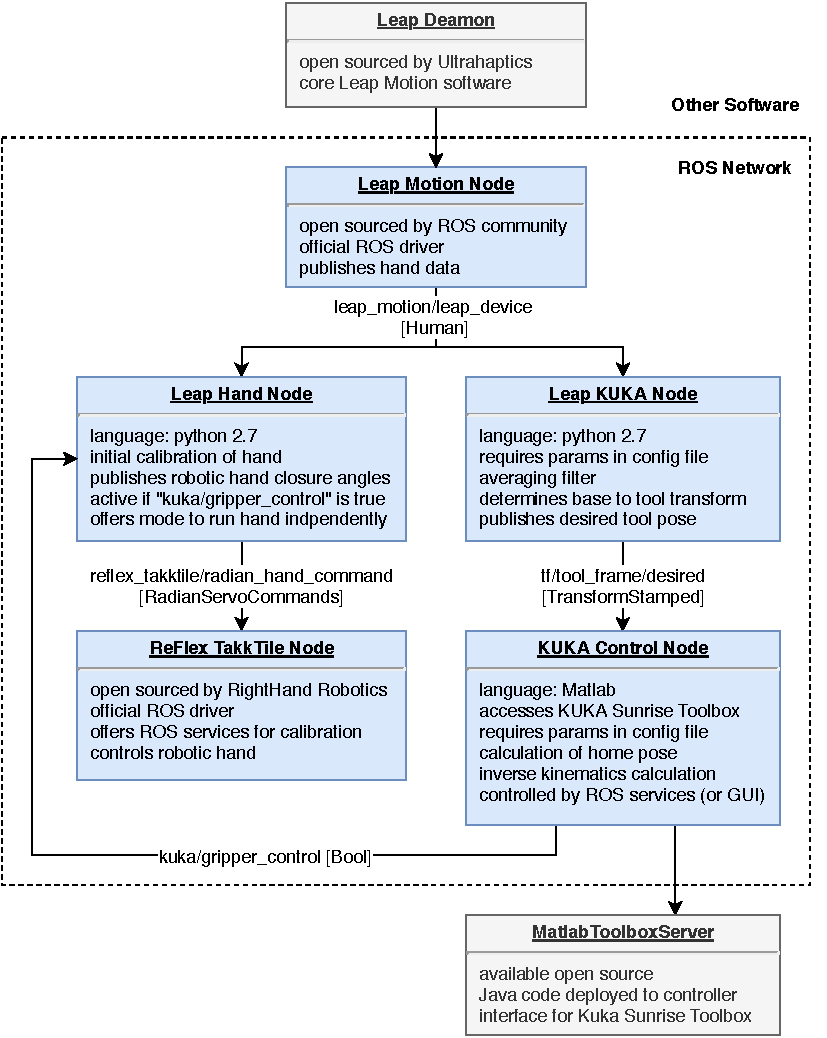
\includegraphics[width=\textwidth]{images/software}
    \caption{Software Architecture: Leap Motion control}
    \label{fig:software_architecture}
\end{figure}

\section{Installation}

This is a step by step guide on how to install the software taken from the README file of the GitHub repository. Note that the above software components first need to be installed.

\begin{figure}[h!]
    \centering
    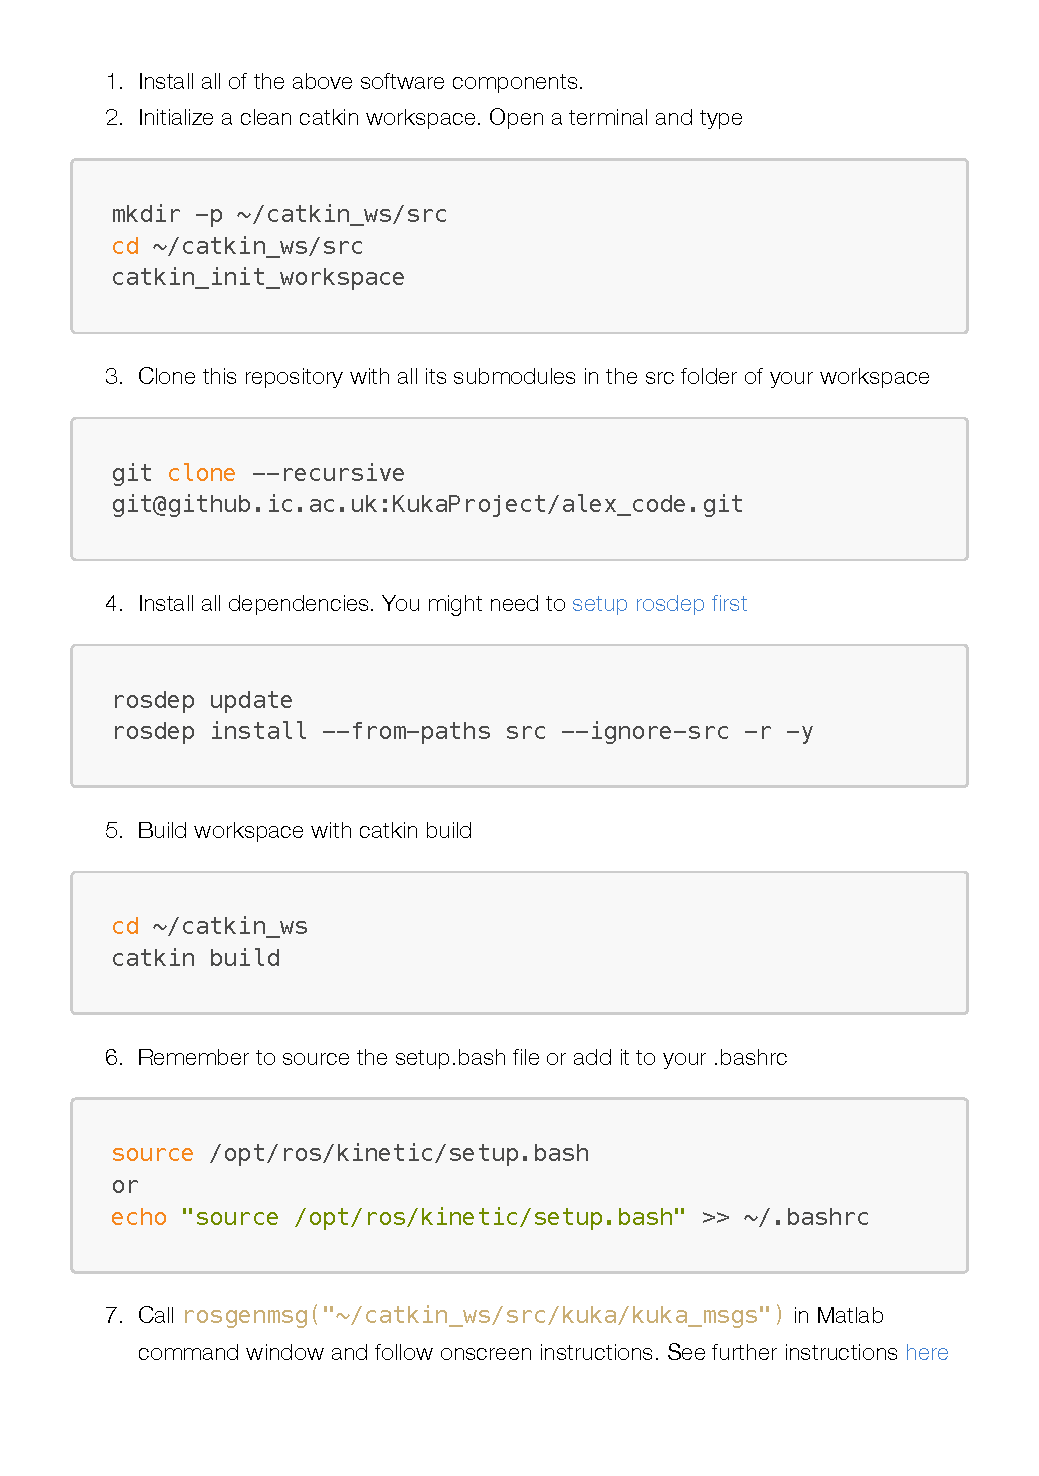
\includegraphics[width=0.85\textwidth]{figures/readme}
\end{figure}

\newpage


\section{Networking Setup}\label{networking}

\begin{figure}[h!]
    \centering
    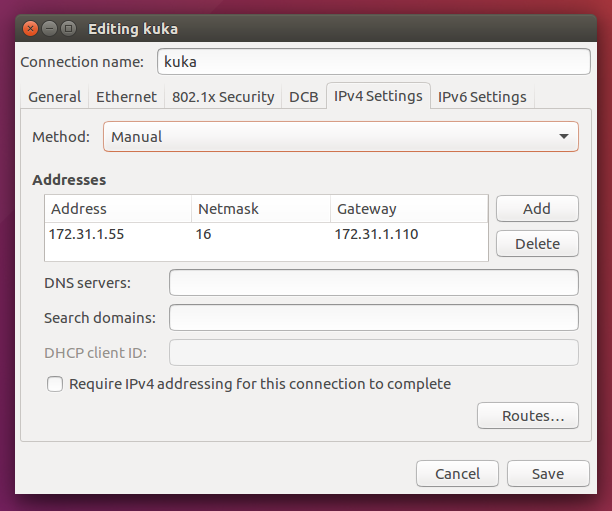
\includegraphics[width=10cm]{figures/network_kuka}
    \caption{Networking setup KUKA}
    \label{fig:net_kuka}
\end{figure}

\begin{figure}[h!]
    \centering
    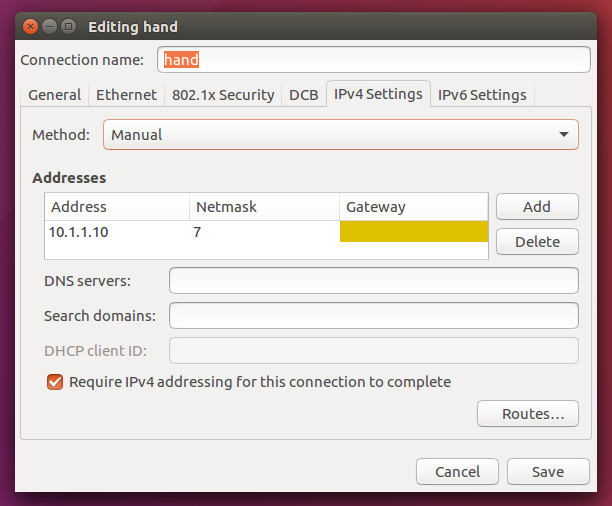
\includegraphics[width=10cm]{figures/network_hand}
    \caption{Networking setup robotic hand}
    \label{fig:net_hand}
\end{figure}

\newpage
\begin{table}[h]
\centering
\begin{tabular}{lll}
\textbf{Setting} & \textbf{KUKA} & \textbf{Robotic Hand} \\
Address          & 172.31.1.55   & 10.1.1.10             \\
Netmask          & 16            & 254.0.0.0             \\
Gateway          & 172.31.1.110  & 0.0.0.0              
\end{tabular}
\caption{Networking settings}
\label{tab:net}
\end{table}

Remember to check "Require IPv4 addressing" button for the robotic hand. Also make sure your ethernet connection shows up as ``eth0''. If it does not \href{https://askubuntu.com/questions/767786/changing-network-interfaces-name-ubuntu-16-04}{this link} might help. Please view the Robotic Hand's \href{https://www.labs.righthandrobotics.com/reflex-quickstart}{documentation} for more details. In their instructions you can skip all sections on cloning and building the drivers as they will already be included in this package. Before you use the networking connections make sure you actually connect to them by clicking on the connections in the networking center.


\section{Folder Structure}

\begin{table}[h]
\centering
\begin{tabular}{ll}
\textbf{Folder Name} & \textbf{Contents}                                                 \\
cad                  & CAD files of 3D printed parts                                     \\
common               & library of common functions used by leap\_hand and leap\_kuka     \\
docs 				 & handbook \\
grasping             & code for autonomous grasping prediction (work in progress)        \\
kuka                 & code for controlling the KUKA robot                               \\
leap\_hand           & code to interface between Leap Motion node and robotic hand node  \\
leap\_kuka           & code to interface between Leap Motion node and KUKA node          \\
leap\_rig            & files to start Leap Motion control of KUKA and robotic hand       \\
modules              & third party software (created upon recursive clone)                                            \\
vision               & all vision related code (camera and virtual reality)
\end{tabular}
\caption{Folder Structure of GitHub repository}
\end{table}

\chapter{KUKA Control Node}

The KUKA control node essentially provides a \gls{ros} wrapper of the Kuka Sunrise Toolbox presented in \cite{Safeea2019}. The Kuka Sunrise Toolbox is a Matlab Toolbox which interfaces with a Java application called MatlabToolboxServer on the KUKA robot controller. The toolbox provides intuitive Matlab functions to control the robot. Figure \ref{fig:kst} shows an overview of the \gls{kst} architecture. 

\begin{figure}[h]
    \centering
    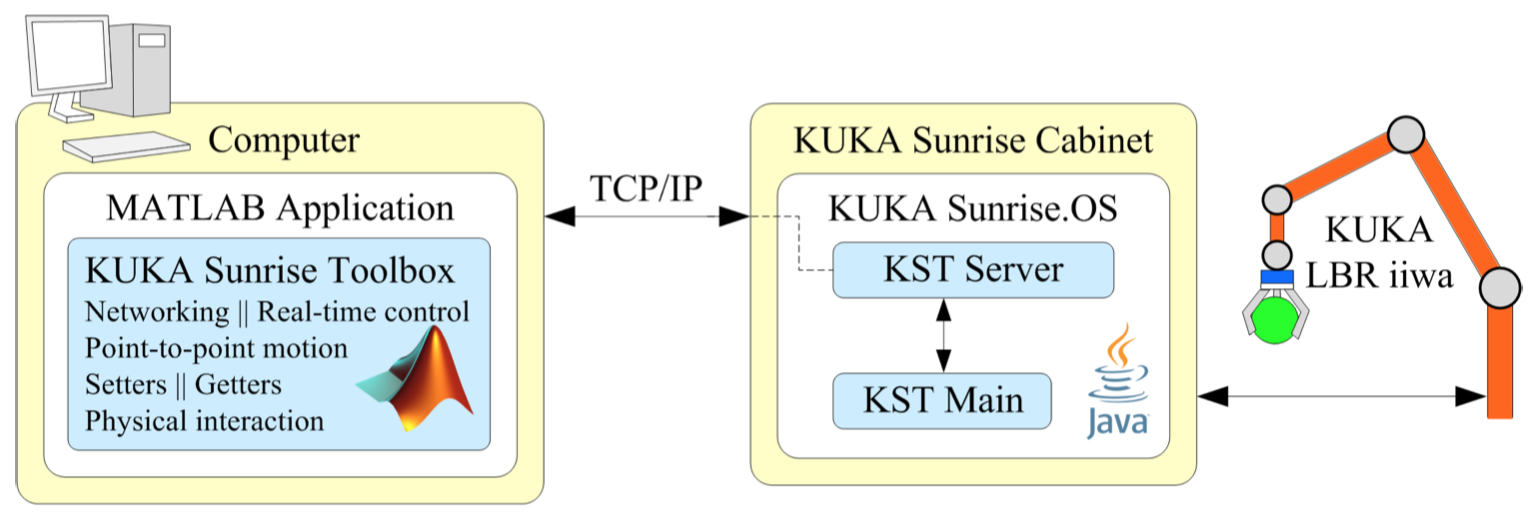
\includegraphics[height=4cm]{images/kst}
    \caption{KUKA Sunrise Toolbox communication scheme \cite{Safeea2019}}
    \label{fig:kst}
\end{figure}

\section{General}

\subsection{Scripts Overview}

The KUKA control package offers four main scripts in the directory \texttt{kuka/kuka\_control/scripts}. The folder \texttt{functions} contains all the relevant functions that are used within these four scripts. 

\begin{table}[h]
\centering
\begin{tabular}{ll}
\textbf{Script Name} & \textbf{Functionality}                                  \\
ptpController.m      & \gls{ros} interface for \gls{ptp} control of the robot              \\
realTimeController.m & \gls{ros} interface for real-time control of the robot        \\
simpleController.m   & short script to send the robot to a joint configuration \\
workspacePlotter.m   & script to plot a workspace defintion                   
\end{tabular}
\caption{Matlab scripts of the KUKA control node}
\label{tab:my-table}
\end{table}

\subsection{KUKA Motion Types}

The two motion types used in this software are \textbf{\gls{ptp} movements} and \textbf{Direct Servo} motions. The \texttt{ptpController.m} script uses only \gls{ptp} movements, whereas the \texttt{realTimeController.m} script uses both methods (movement to the home position, zero position, the mirroring pickup point in \gls{ptp} mode, otherwise in real-time mode). Direct Servo is a functionality issued by KUKA to allow for "soft" real-time control of the robot in joint space. The documentation about the Direct Servo motion type is quite sparse, unfortunately. Any motions executed with the Direct Servo functionality are referred to as real-time motions in this report.

This is a description of \gls{ptp} movements taken from the KUKA manual. "The robot guides the TCP along the fastest path to the end point. The fastest path is generally not the shortest path in space and is thus not a straight line. As the motions of the robot axes are simultaneous and rotational, curved paths can be executed faster than straight paths. \gls{ptp} is a fast positioning motion. The exact path of the motion is not predictable, but is always the same, as long as the general conditions are not changed" \cite[p.~303]{KukaManual}.

Below you can get a graphical intuition of the \gls{ptp} motion type as opposed to the linear motion type (which is not used in the software). In the LIN motion type the "robot guides the TCP at the defined velocity along a straight path in space to the end point" \cite[p.~304]{KukaManual}. 

\begin{figure}[h]
    \centering
    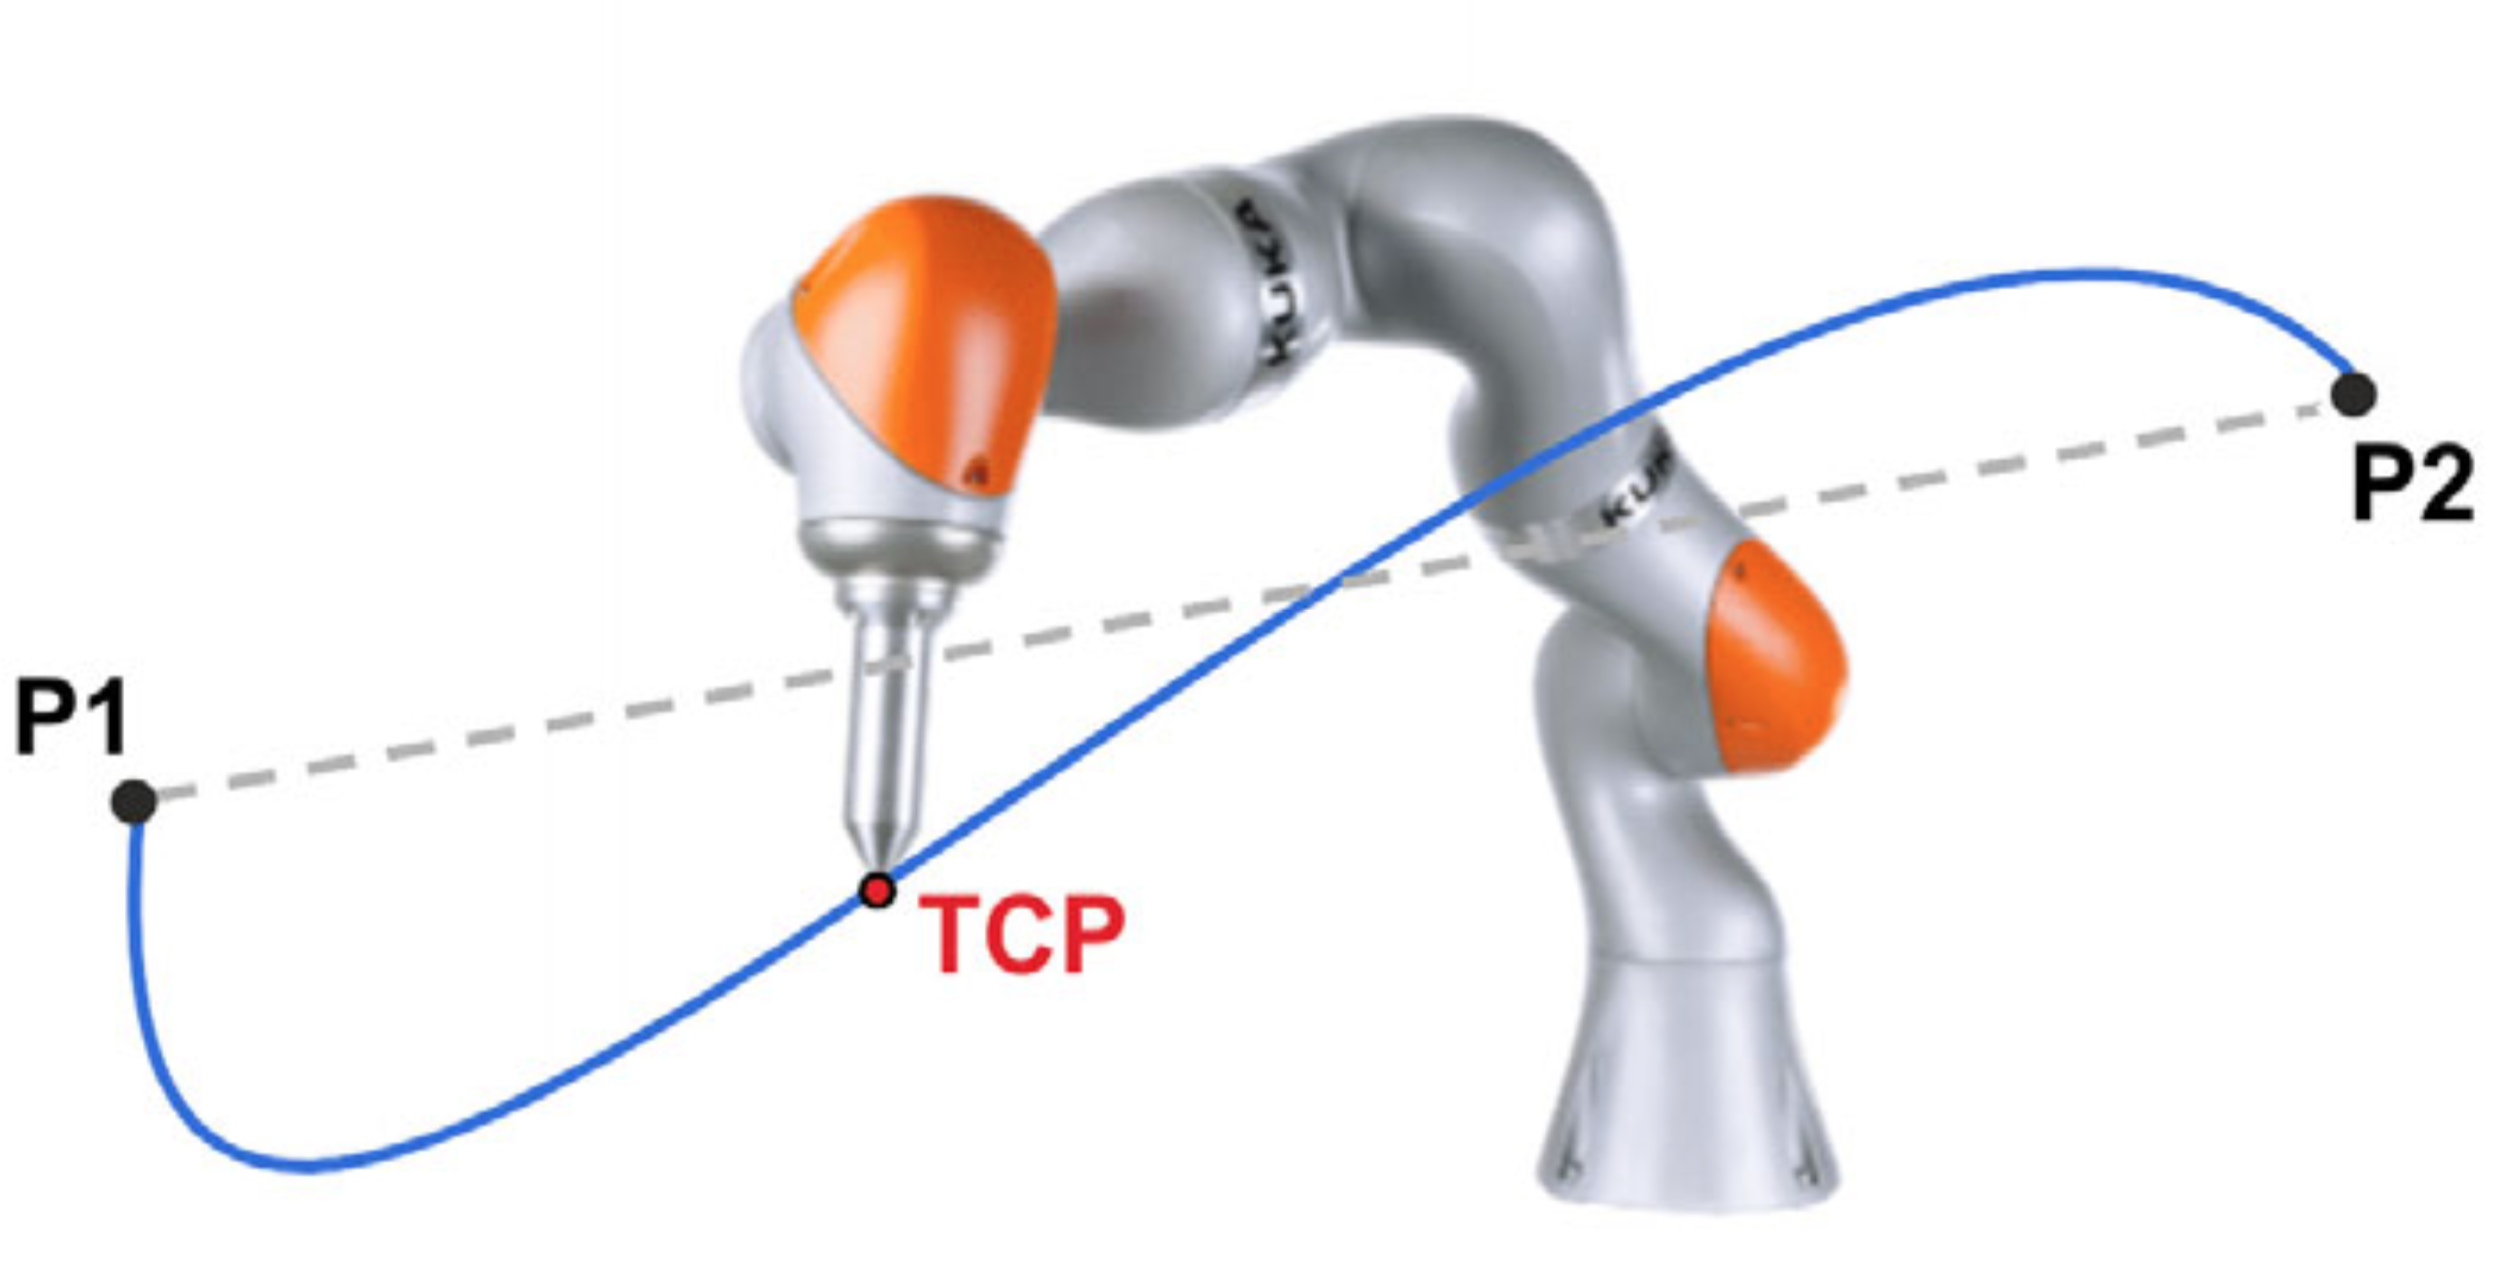
\includegraphics[height=4cm]{images/ptp_motion}
    \caption{PTP Motion \cite[p.~304]{KukaManual}}
    \label{fig:ptp_motion}
\end{figure}
\begin{figure}[h]
    \centering
    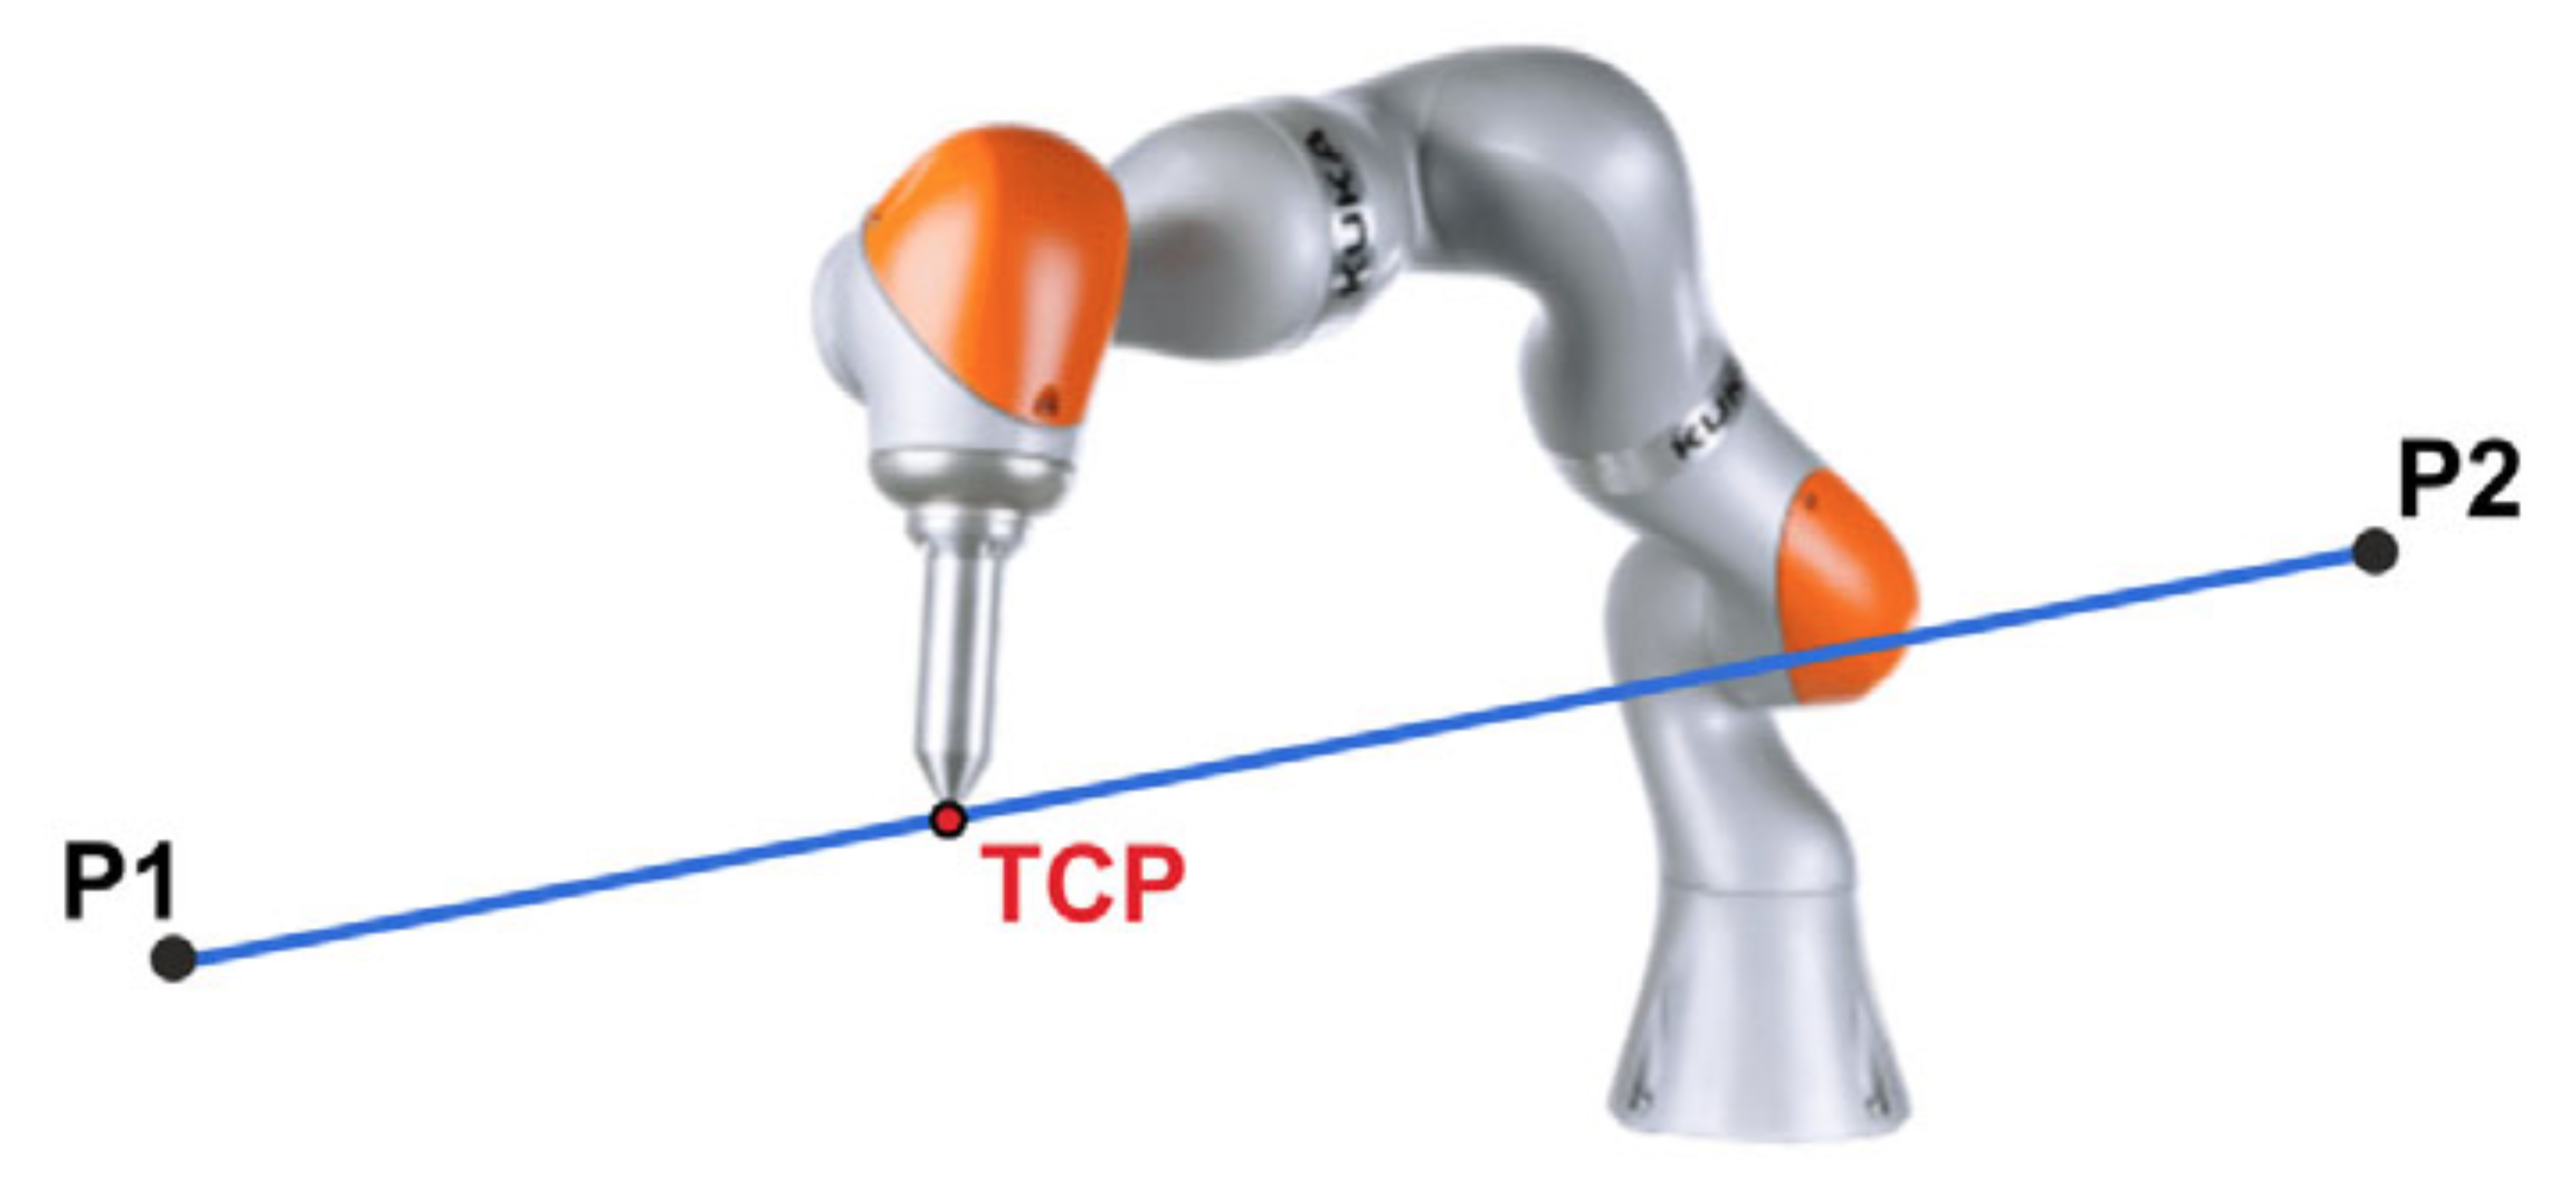
\includegraphics[height=4cm]{images/lin_motion}
    \caption{LIN Motion \cite[p.~304]{KukaManual}}
    \label{fig:lin_motion}
\end{figure}

The \gls{ptp} and real-time \gls{ros} nodes use the functions \texttt{movePTPJointSpace(jPos, relVel)} and \texttt{sendJointsPositionsf(jPos)} that are offered by the \gls{kst} to move the robot. The \texttt{jPos} variable is a 1x7 cell array of target joint positions. The \texttt{relVel} variable specifies the relative motion execution speed (i.e. a value from 0 to 1, with 1 indicating maximum speed). Please refer to the KST's user manual in their \href{https://github.com/Modi1987/KST-Kuka-Sunrise-Toolbox}{GitHub repository} for more information.

\subsection{Services of Control Scripts}

Both the \texttt{ptpController.m} and the \texttt{realTimeController.m} script have exactly the same \gls{ros} interface. They can both be controlled with \gls{ros} services or a Graphical User Interface. Table \ref{tab:services} shows a list of the services provided by the script. When the \gls{ros} services are called (like shown in Listing \ref{code:services}) the user will receive a feedback message, if the service call was successfully executed (also see Figure \ref{fig:services}).

\begin{table}[h]
\centering
\begin{tabular}{lll}
\textbf{Service Name}     & \textbf{Service Type}        & \textbf{Description}          \\
kuka/exit\_app\_emergency & kuka\_msgs/exitAppEmergency  & terminate Matlab              \\
kuka/exit\_app            & kuka\_msgs/exitApp           & shutdown control script       \\
kuka/kuka\_control        & kuka\_msgs/setKukaControl    & switch KUKA control on/off    \\
kuka/gripper\_control     & kuka\_msgs/setGripperControl & switch gripper control on/off \\
kuka/scaling\_factor      & kuka\_msgs/setScalingFactor  & scale translation     
\end{tabular}
\caption{ROS services provided by the KUKA control nodes}
\label{tab:services}
\end{table}

\begin{lstlisting}[language=bash, caption={Usage of \gls{ros} services}, captionpos=b, label=code:services]

rosservice call kuka/exit_app_emergency
rosservice call kuka/exit_app
rosservice call kuka/kuka_control true
rosservice call kuka/gripper_control true
rosservice call kuka/scaling_factor 0.7

\end{lstlisting}

All services become available once either the \texttt{ptpController.m} or the \texttt{realTimeController.m} Matlab script is run. Use the \texttt{exit\_app} service to shut down the connection to the robot controller and terminate Matlab. The \texttt{exit\_app\_emergency} service will terminate Matlab immediately without shutting down the robot connection. The \texttt{kuka\_control} service is used to enter either \gls{ptp} or real-time control mode (depending on which script is running). With the \texttt{gripper\_control} service the boolean which is published on the \texttt{kuka/gripper\_control} \gls{ros} topic can be changed. The fact that users have to activate the control of the KUKA and the gripper once the control script is running can be seen as a safety measure to avoid unintentional motions. The range in which movements can be scaled is 0.1 to 1.5. It is not encouraged to change this to ensure safety.

\begin{figure}[h]
    \centering
    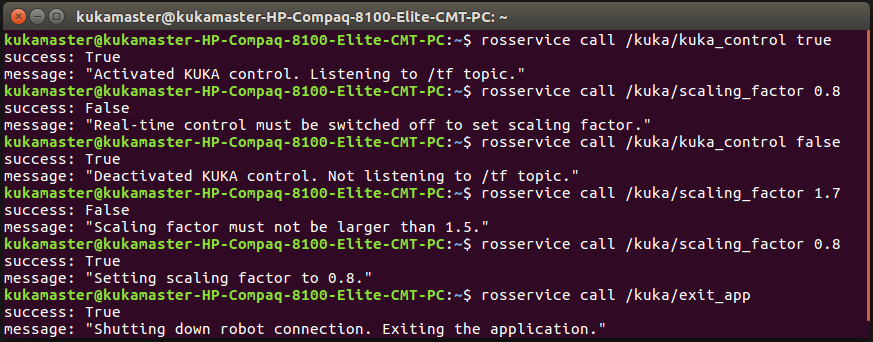
\includegraphics[height=5.5cm]{figures/services}
    \caption{Feedback of \gls{ros} services}
    \label{fig:services}
\end{figure}

The Graphical User Interface in Figure \ref{fig:gui} can also be used to control the software. Each service corresponds to a button on the \gls{gui} (except the "Reset Scaling Factor" button). The slider in the \gls{gui} makes the scaling factor continuously adjustable. The "ROS Control" buttons in the KUKA and Gripper panels will turn green once the respective functionality is actually available (also turns green if activated through service call). This gives an intuitive graphical feedback in which state the software is currently in.

\begin{figure}[h]
    \centering
    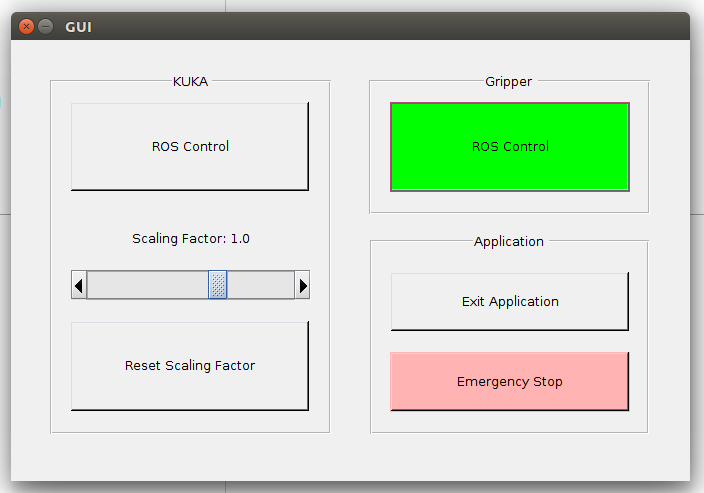
\includegraphics[height=7.5cm]{figures/gui}
    \caption{Graphical user interface}
    \label{fig:gui}
\end{figure}

\newpage
\subsection{Topics of Control Scripts}

When either the \texttt{ptpController.m} or the \texttt{realTimeController.m} is run the below \gls{ros} topics become available and data about the robot state is published. Especially notable is the \texttt{kuka/gripper\_control} topic, which indicates the status of an attached gripper (see chapter \ref{hand}). All transforms published are in the KUKA base frame and can be conveniently accessed in the \gls{ros} tf tree. 

Note that all messages of the \texttt{kuka\_msgs/} type and the \texttt{tf/kuka/flange\_frame/measured} can not be provided while the robot moves in real-time mode. The topics will still exist, but while real-time movements are executed no new messages will be published to these topics. The reason for this is that when in real-time mode, the \gls{kst} does not allow to request the robot state. This only works reliably when in \gls{ptp} mode. Possibly, the \gls{kst} will be updated in the future with functions to allow for this (see chapter \ref{future}).

\begin{table}[h]
\centering
\begin{tabular}{ll}
\textbf{Topic Name}            & \textbf{Message Type}           \\
kuka/gripper\_control          & std\_msgs/Bool                  \\
kuka/moving\_rt                & std\_msgs/Bool                  \\
kuka/moving\_ptp               & std\_msgs/Bool                  \\
tf/kuka/flange\_frame/home     & geometry\_msgs/TransformStamped \\
tf/kuka/tool\_frame/home       & geometry\_msgs/TransformStamped \\
tf/kuka/flange\_frame/measured & geometry\_msgs/TransformStamped \\
kuka/flange\_force             & geometry\_msgs/Vector3Stamped   \\
kuka/flange\_torque            & geometry\_msgs/Vector3Stamped   \\
kuka/joint\_positions          & kuka\_msgs/jointPositions       \\
kuka/joint\_torques\_external  & kuka\_msgs/jointTorquesExternal \\
kuka/joint\_torques\_measured  & kuka\_msgs/jointTorquesMeasured
\end{tabular}
\caption{ROS messages published by the KUKA control node}
\label{tab:my-table}
\end{table}

To move the robot using the KUKA control node a stream of \gls{ros} \texttt{geometry\_msgs/TransformStamped} messages from \texttt{kuka/base\_frame} to \texttt{kuka/tool\_frame/desired} should be published to the \gls{ros} network. This is the only topic the \gls{ros} node subscribes to.

\newpage
\subsection{KUKA Configuration File}

The following parameters have to be set in the configuration file called \texttt{kuka\_params\_ptp.yaml} or \texttt{kuka\_params\_rt.yaml} depending on the control script you are using. The parameters must be uploaded to the \gls{ros} parameter server before running the control scripts. This can be done with the included launch files \texttt{kuka\_params\_ptp.launch} or \texttt{kuka\_params\_rt.launch}. The parameters's units are meters, degrees and seconds. 

\begin{table}[h]
\centering
\begin{tabular}{llll}
\textbf{Mode} & \textbf{Parameter Name} & \textbf{Default}                & \textbf{Note}                     \\

both          & robot                   & LBR7R800	                      & LBR7R800 or LBR14R820             \\
both          & flange                  & MF\_elektrisch                   & MF\_elektrisch, MF\_pneumatisch,\\&&& MF\_IO\_pneumatisch or \\&&&MF\_touch\_pneumatisch\\
both          & ip                      & 172.31.1.147                    & robot ip                                 \\
both          & center\_line            & {[}1, -1, 0	  {]}             & z must be zero               \\
both          & opening\_angle          & 50.0                            & range (0, 180)                    \\
both          & z\_lower\_limit         & 0.2                             & range (0.1, z\_upper\_limit)      \\
both          & z\_upper\_limit         & 0.6                             & range (z\_lower\_limit, 1.14)     \\
both          & inner\_sphere\_limit    & 0.5                             & range (0.4, outer\_sphere\_limit) \\
both          & outer\_sphere\_limit    & 0.7                             & range (inner\_sphere\_limit, 0.8) \\
both          & tool\_length            & 0.106                           & range {[}0, inf)                  \\
both 		  & time\_out				& 0.2						      & move home after time\_out \\
both          & home\_pos               & {[}-45, 30, 0, -80, 0, 70, 0{]} & disregard if use\_home\_pos false         \\
both          & use\_home\_pos       & false                           & use home\_pos param or not        \\
rt            & velocity\_ptp\_slow     & 0.15                            & range (0, 1)                      \\
rt            & velocity\_ptp\_fast     & 0.25                            & range (0, 1)                      \\
ptp           & velocity\_ptp           & 0.15                            & range (0, 1)                      \\
ptp           & joints\_thresh          & 0.5                             & if below not moving              
\end{tabular}
\caption{KUKA configuration parameters}
\label{tab:kuka_config}
\end{table}

The \texttt{time\_out} parameter specifies after what time the robot moves back to its home position if the KUKA node does not receive any more new tf messages. The node always measures the time from the last received \gls{ros} time stamp. If a "new" message is received (i.e. time stamp differs from previous message) the timer is reset. If you set the \texttt{time\_out} parameter to a high number (e.g. 999999 seconds) the robot will stay in position that corresponds to last message and not move home until the set \texttt{time\_out} is reached. When you publish new tool transforms to the KUKA control node, be sure that the pose is close to the one when you left off. In future work the robot should rather do a PTP motion to the new pickup point (see chapter \ref{future}). 

In the current state of the software it is only possible to define the tool length and not a full transformation matrix from flange to tool. This is to keep calculations of the home pose simple. The tool length is measured along the flange's Z axis. Since the tool is fixed to the flange, the rotation of flange and tool is identical. If a tool length of 0 is set the flange frame will be controlled.

It is the operators responsibility to ensure that using the provided parameters the robot can reach all positions in the workspace. If the robot can not reach a position it will stay in its previous pose. 

\subsection{Workspace Definition}\label{ws_def}

Since the working envelope of the KUKA robot follows the shape of a hollow sphere (grey area in Figure \ref{fig:ws_params_side}) it was decided that the workspace boundary should be a segment of this spherical shape. The workspace of the robot is defined by the parameters \texttt{center\_line}, \texttt{opening\_angle}, \texttt{z\_lower\_limit}, \texttt{z\_upper\_limit}, \texttt{inner\_sphere\_limit} and \texttt{outer\_sphere\_limit}. Figures \ref{fig:ws_params_side} and \ref{fig:ws_params_top} show an overview of what the individual workspace parameters mean.

It is encouraged to visualise the workspace with the Matlab script \texttt{workspacePlotter.m} before editing the configuration file. Figure \ref{fig:ws_plot_1} shows a workspace plot. For the plot many random positions are sampled and then constrained using the function \texttt{getConstrainedPosition.m}, which is also used in the control scripts. The visualisation also shows the calculated workspace center and the home pose of both the tool and flange frame. The tool tip (center of frame) always coincides with the workspace center (red dot in Figure \ref{fig:ws_plot_1}) when the robot reaches its home position. Also view Figure \ref{fig:ws_plot_2} to see the visualisation of another possible workspace.

Please see the below conventions for coordinate systems (Figure \ref{img:kuka_coosy}) and joint conventions (Figure \ref{img:kuka_convention}) which are used throughout this software. The KUKA manual describes the joint convention as follows. "The positive direction of rotation of the robot axes can be determined using the right-hand rule. Imagine the cable bundle which runs inside the robot from the base to the flange. Mentally close the fingers of your right hand around the cable bundle at the axis in question. Keep your thumb extended while doing so. Your thumb is now positioned on the cable bundle so that it points in the same direction as the cable bundle runs inside the axis on its way to the flange. The other fingers of your right hand point in the positive direction of rotation of the robot axis" \cite[p.~87]{KukaManual}.

For labelling axes the standard "XYZ-RGB" convention is used in this report.

\begin{enumerate}
	\item X axis corresponds to red color
	\item Y axis corresponds to green color
	\item Z axis corresponds to blue color 
\end{enumerate}

\newpage
\begin{figure}[h!]
    \centering
    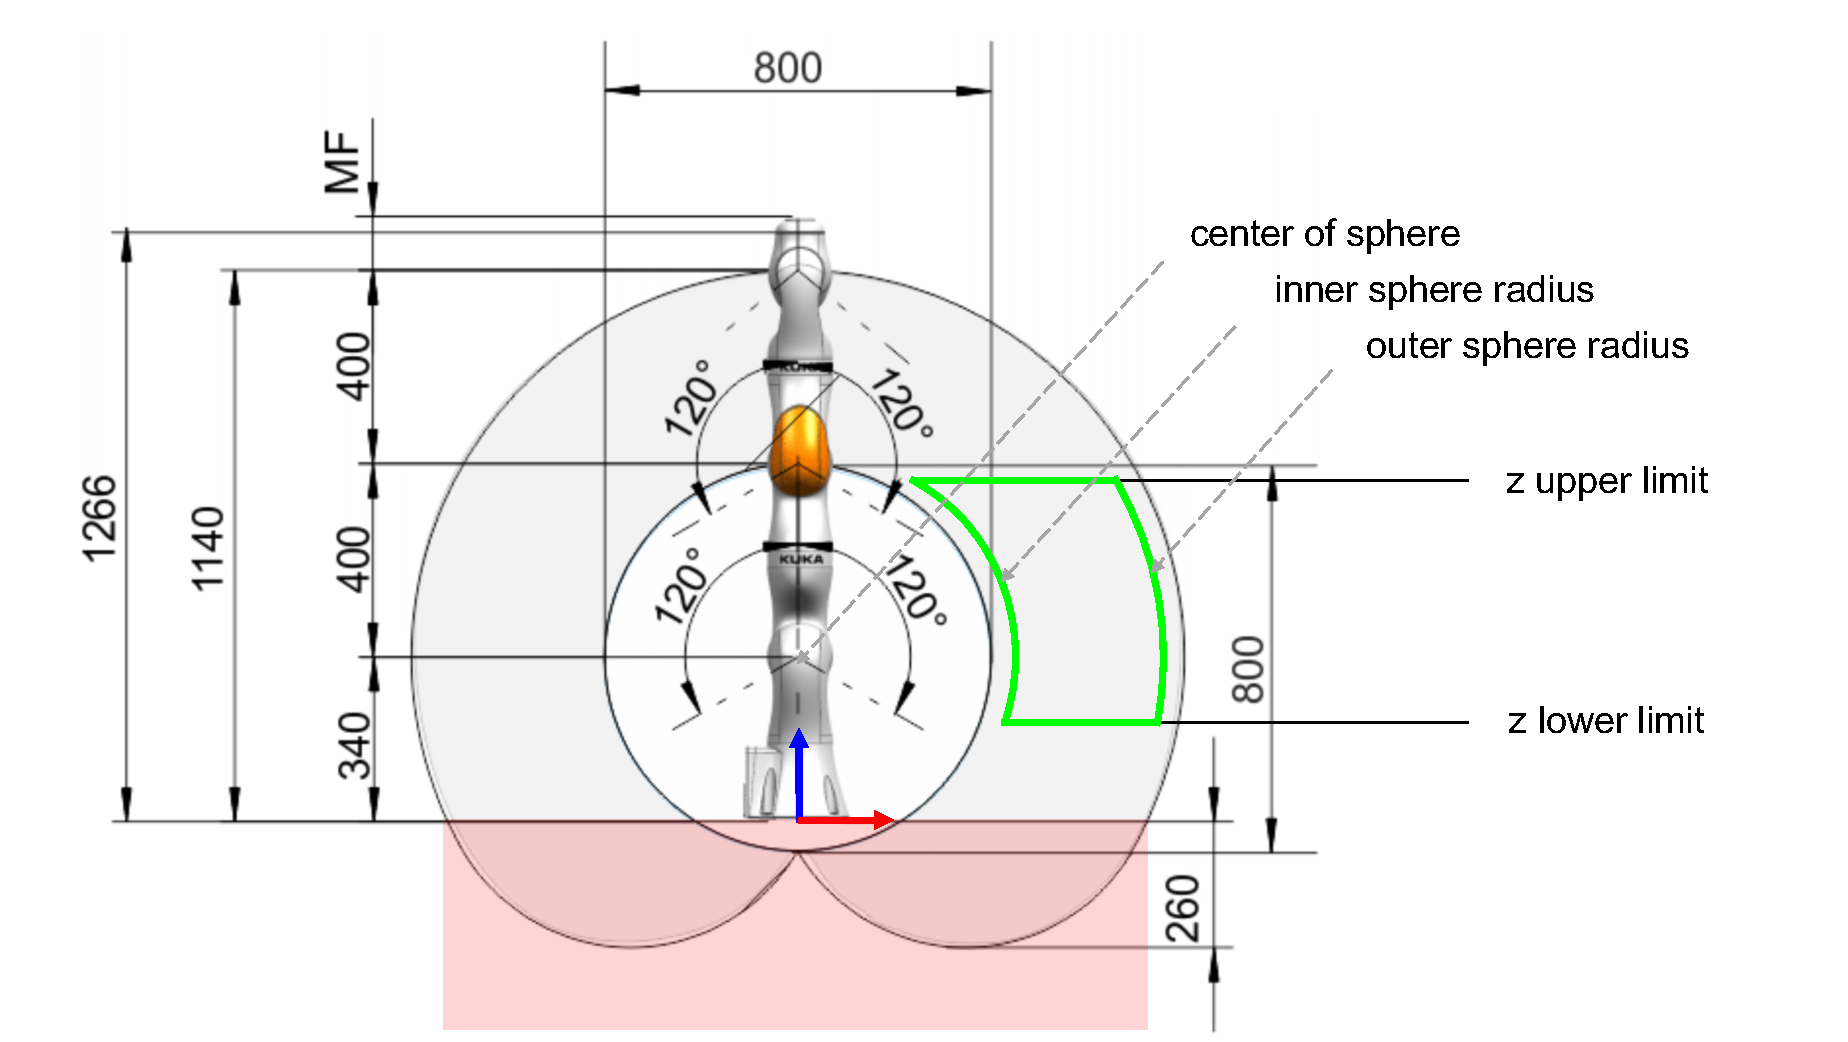
\includegraphics[height=8cm]{images/ws_params_side}
    \caption{Workspace parameters (side view) \cite[p.~36]{KukaManualFlange}}
    \label{fig:ws_params_side}
\end{figure}

\begin{figure}[h!]
    \centering
    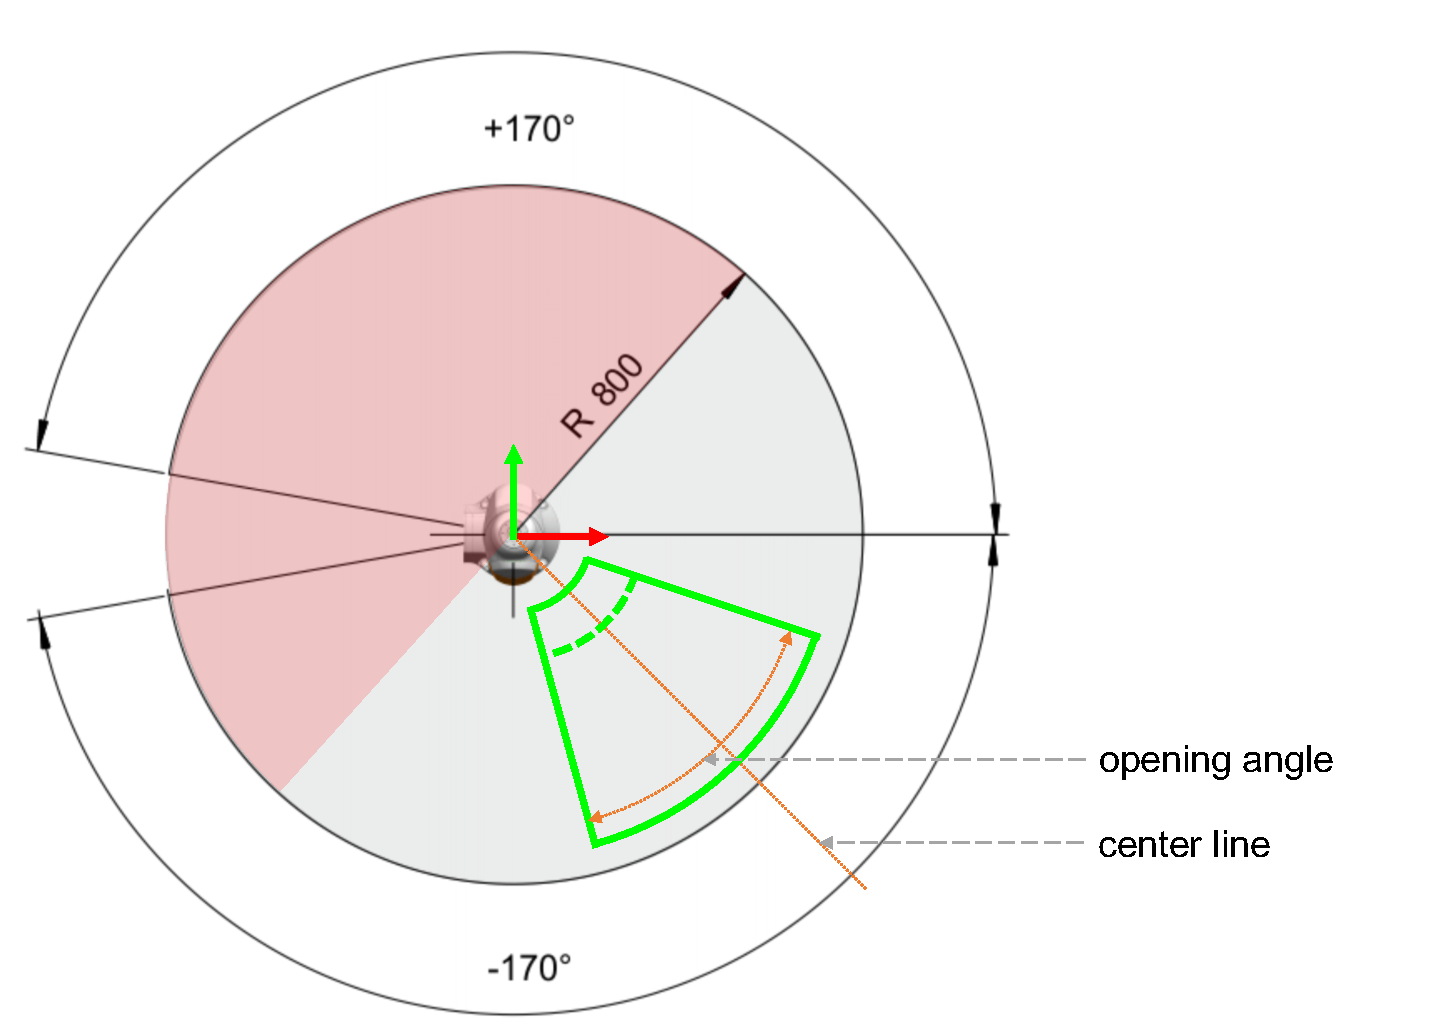
\includegraphics[height=8cm]{images/ws_params_top}
    \caption{Workspace parameters (top view) \cite[p.~36]{KukaManualFlange}}
    \label{fig:ws_params_top}
\end{figure}

\newpage

\begin{figure}[h!]
    \centering
    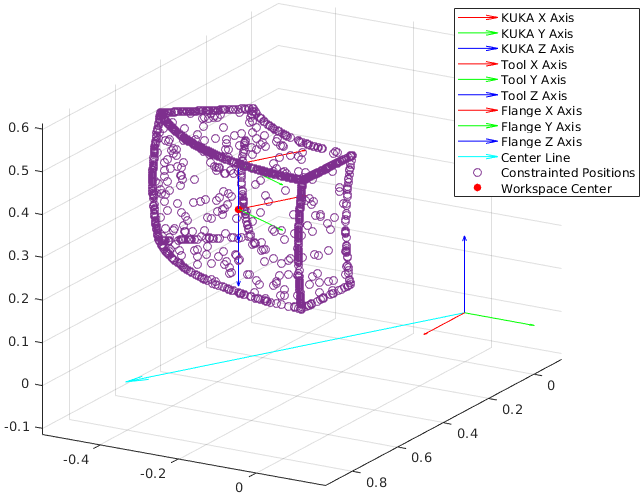
\includegraphics[height=8cm]{figures/ws_1}
    \caption{Workspace plot (center line [2,-1,0], opening angle 50 deg)}
    \label{fig:ws_plot_1}
\end{figure}

\begin{figure}[h!]
    \centering
    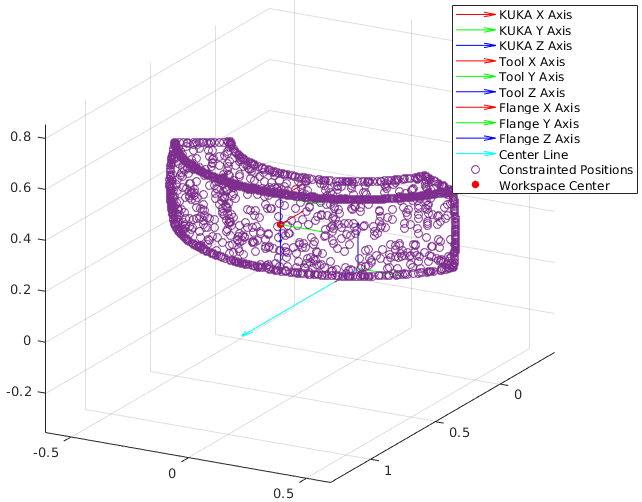
\includegraphics[height=8cm]{figures/ws_2}
    \caption{Workspace plot (center line [1,0,0], opening angle 120 deg)}
    \label{fig:ws_plot_2}
\end{figure}
\newpage

\begin{figure} [h]
\centering
\begin{minipage}{.4\textwidth}
  \centering
  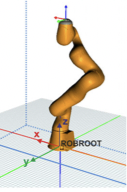
\includegraphics[height=7.5cm]{images/kuka_coosy}
  \captionof{figure}{Coordinate systems \cite{KukaManual}}
  \label{img:kuka_coosy}
\end{minipage}
\begin{minipage}{.4\textwidth}
  \centering
  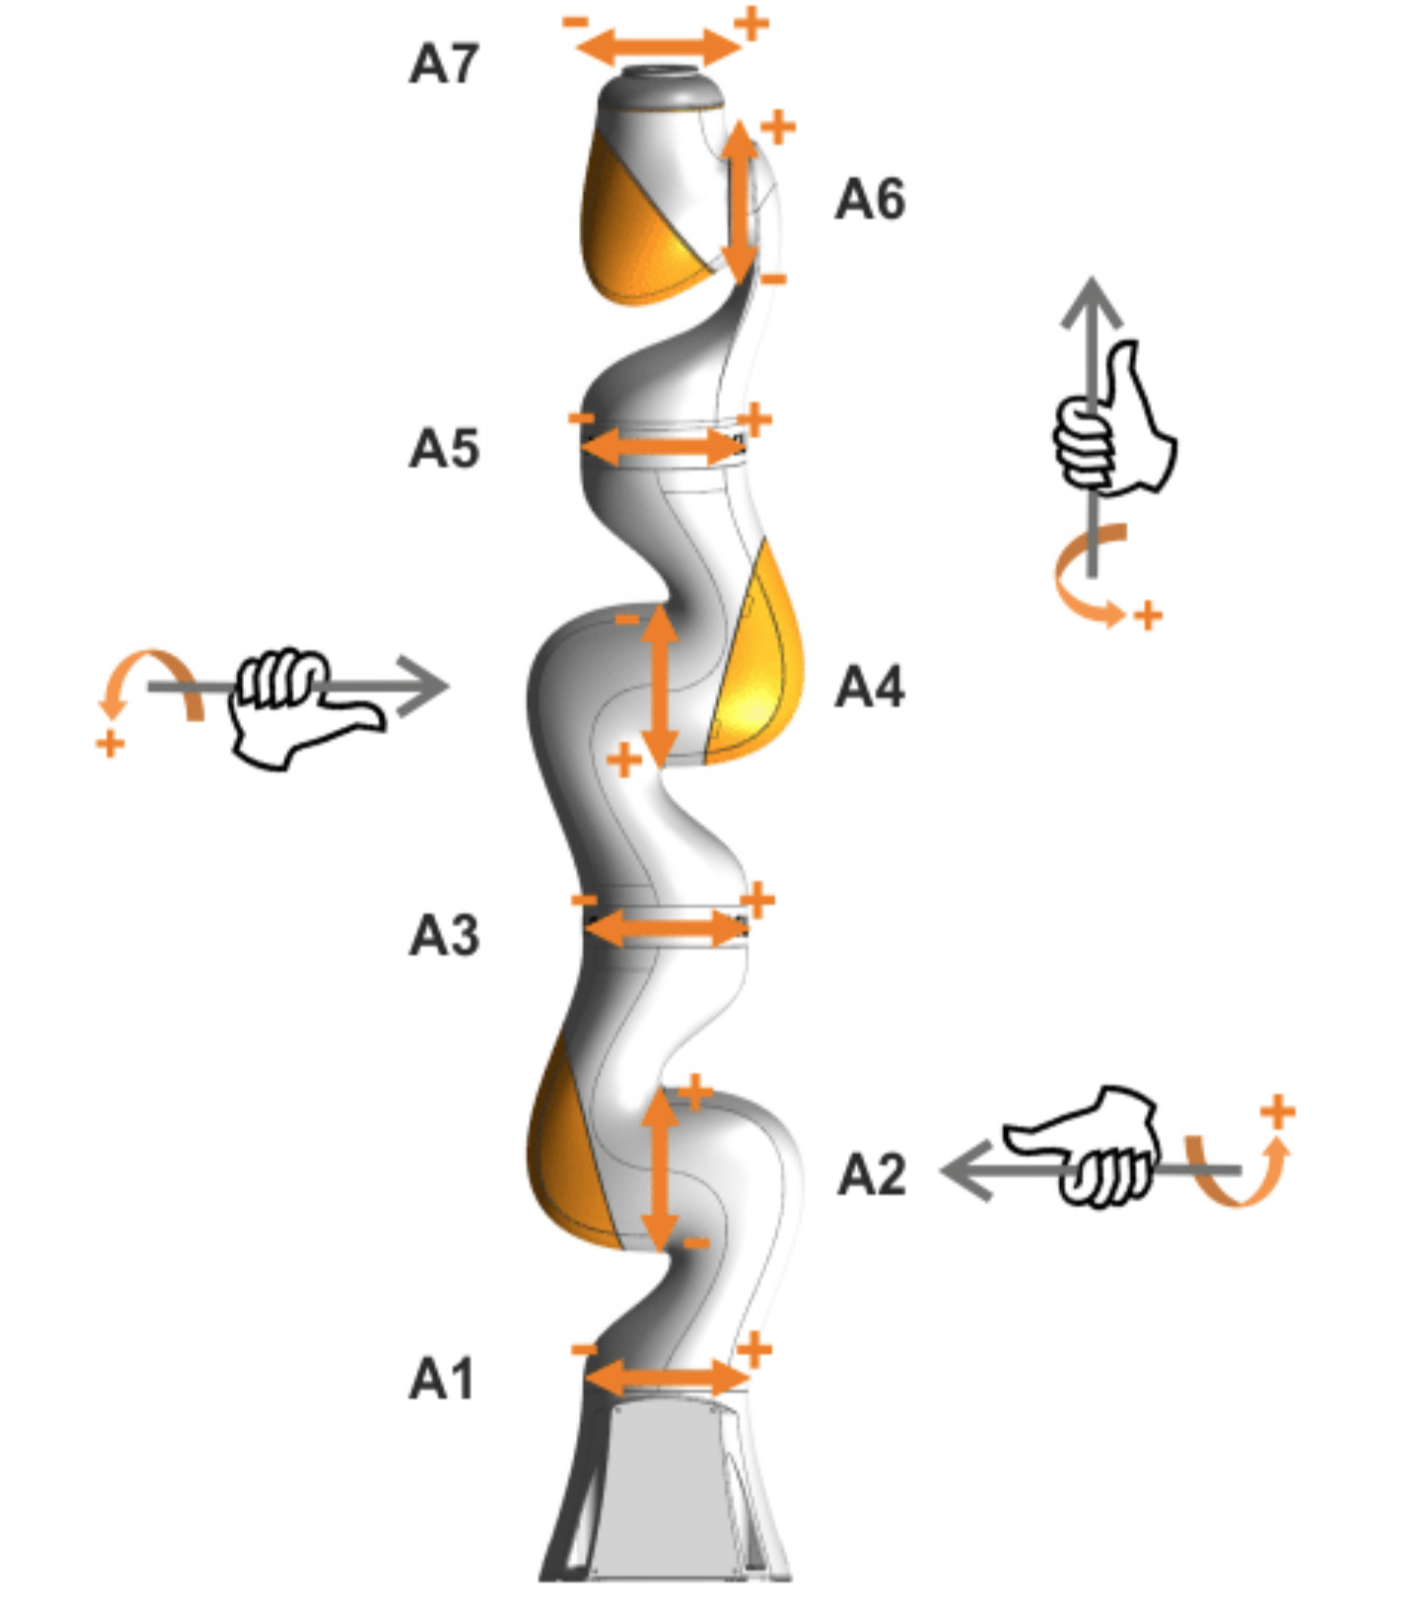
\includegraphics[height=7.5cm]{images/kuka_convention}
  \captionof{figure}{Joint convention \cite{KukaManual}}
  \label{img:kuka_convention}
\end{minipage}
\end{figure}

\subsection{Enforcing Workspace Boundary}

During execution of the control scripts the \texttt{getConstrainedPosition.m} function is used to limit the position of the tool. There are four main parts to the enforcement of the workspace boundary. 
\begin{enumerate}
	\item If the desired tool position is above/below the allowed Z limits the constrained position is projected down/up along the shortest path to the allowed Z limit (shortest path is always along z axis). The range of motion in the XY plane is not restricted unless no other boundary constraint is enforced.
	\item If the desired tool position is further from/closer to the origin of joint 2 than the allowed spherical limits the position is projected back to a valid position along a vector pointing perpendicular from the z axis to the desired position.
	\item If the desired tool position is beyond the planes which are defined by the center line and the opening angle, the position will be projected down to the closest valid point on the workspace boundary (along normal of these planes).
	\item If the desired tool position lies within any of the red areas in figures \ref{fig:ws_params_side} and \ref{fig:ws_params_top} (i.e. in negative center line direction or in negative z direction) an error is thrown. This is a safety precaution as positions that lie within these areas are unfeasible and might potentially be dangerous. If the control scripts recognise such an error the application is shutdown.
\end{enumerate}

\newpage

\subsection{Home Position Calculation}\label{home_calc}

In this software the home pose is always the idle position that the robot reaches when the application is started. The zero position is the position in which the arm is fully stretched out (i.e. joint positions [0, 0, 0, 0, 0, 0, 0]). This position is reached when the script successfully shuts down.

Note that the home position is not calculated if the parameter \texttt{use\_home\_pos} equals to true. If it equals to true the system will take whatever home position is specified by the \texttt{home\_pos} parameter. The given home position must lead to a tool position that lies within the defined workspace. The workspace center parameter is set to the cartesian tool home position (as the software scales around this point). The workspace center is uploaded to the \gls{ros} parameter server by the control script and hence becomes visible to other nodes.

If the \texttt{use\_home\_pos} parameter equals to false, the home position will be calculated from the workspace definition and corresponding to the below constraints. 

\begin{enumerate}
	\item Tool position must coincide with workspace center
	\item Tool Z axis must point downwards
	\item Tool X axis must align with workspace center line
	\item All joints must lie in plane spanned by center line and KUKA Z axis 
	\item Joints 3, 5 and 7 are fixed (i.e. 0) 
\end{enumerate}

The following paragraphs describe how the workspace is calculated if the \texttt{use\_home\_pos} parameter equals to false. Firstly, the workspace center is calculated like Figure \ref{fig:ws_center} shows. The function \texttt{getJointsHome.m} computes the home pose from the workspace center and the above constraints. It simplifies the inverse kinematics problem to a 2R planar robot. Joint position 1 is calculated such that the rotation axis of joint 2 is perpendicular to the simplification plane in Figure \ref{fig:home_position}. The simplification plane is spanned by the specified center line and the KUKA Z axis. Joint position 2 and 4 are calculated such that joint 6 lies in its correct position (above workspace center). The elbow up solution is chosen. Joint 6 is calculated such that tool Z axis faces downwards.

The script throws an error when the given workspace parameters would lead to a non-reachable home pose. A reason for this might be that the tool length that was specified is too long.

\begin{figure}[h]
    \centering
    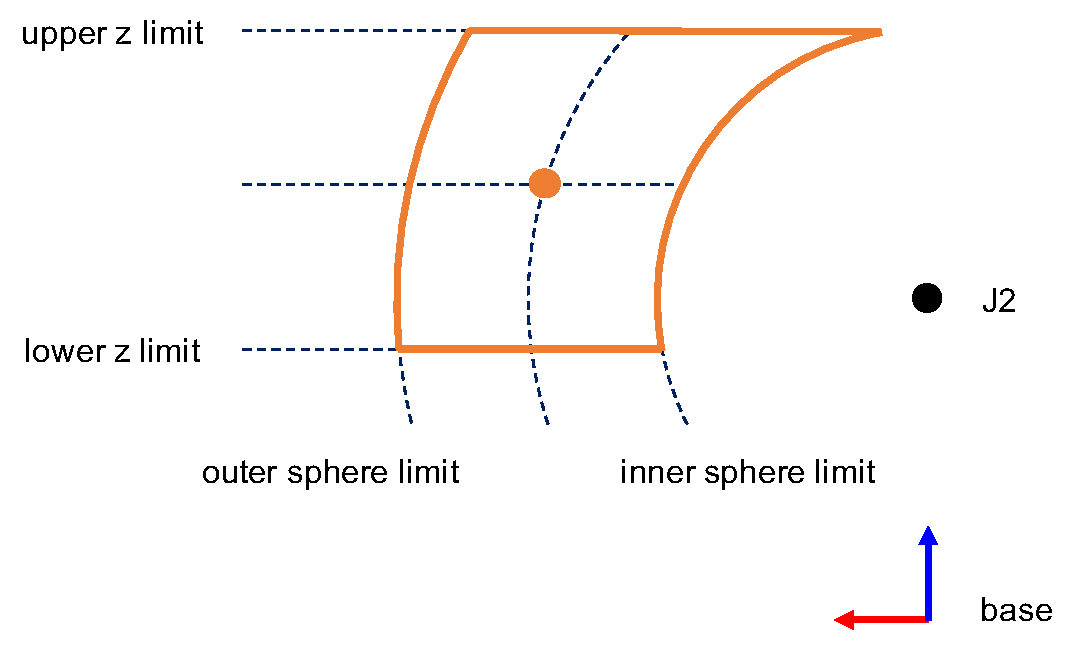
\includegraphics[width=11cm]{images/ws_center}
    \caption{Calculation of workspace center}
    \label{fig:ws_center}
\end{figure}

\newpage
Since a 360 degree variability is required but the limits of joint 1 are +/- 170 degrees two cases are distinguished (see Figure \ref{fig:home_position}). If the center line points in the positive X direction (including [0,1,0] and [0,-1,0]) the home position will resemble the left picture (also see Figure \ref{case_1}). If the center line points in the negative X direction the home position will resemble the right illustration (also see Figure \ref{case_2}). Depending on which home pose is initially calculated (tool X axis points towards or away from base frame) the operator needs to publish the correct desired tool frame transform to the system.

\begin{figure}[h!]
    \centering
    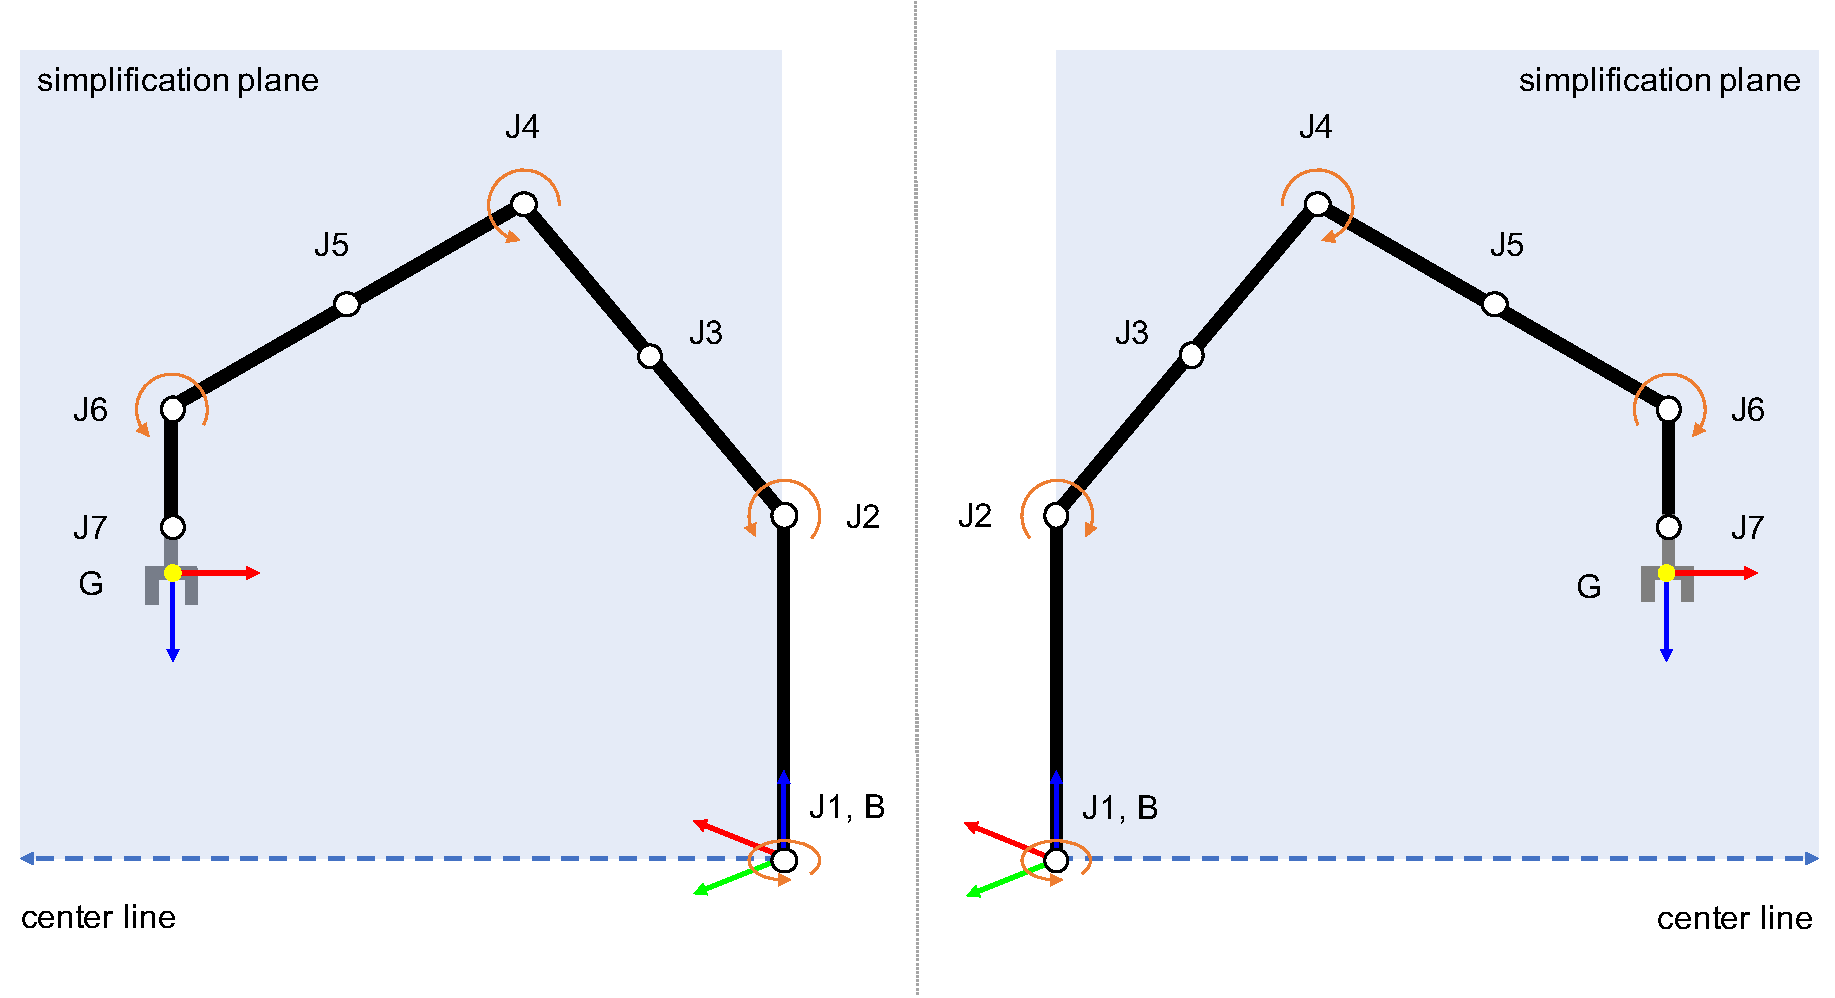
\includegraphics[width=\textwidth]{images/home_position}
    \caption{Calculation of home position}
    \label{fig:home_position}
\end{figure}

\newpage
\vfill
\begin{figure}[h!]
    \centering
    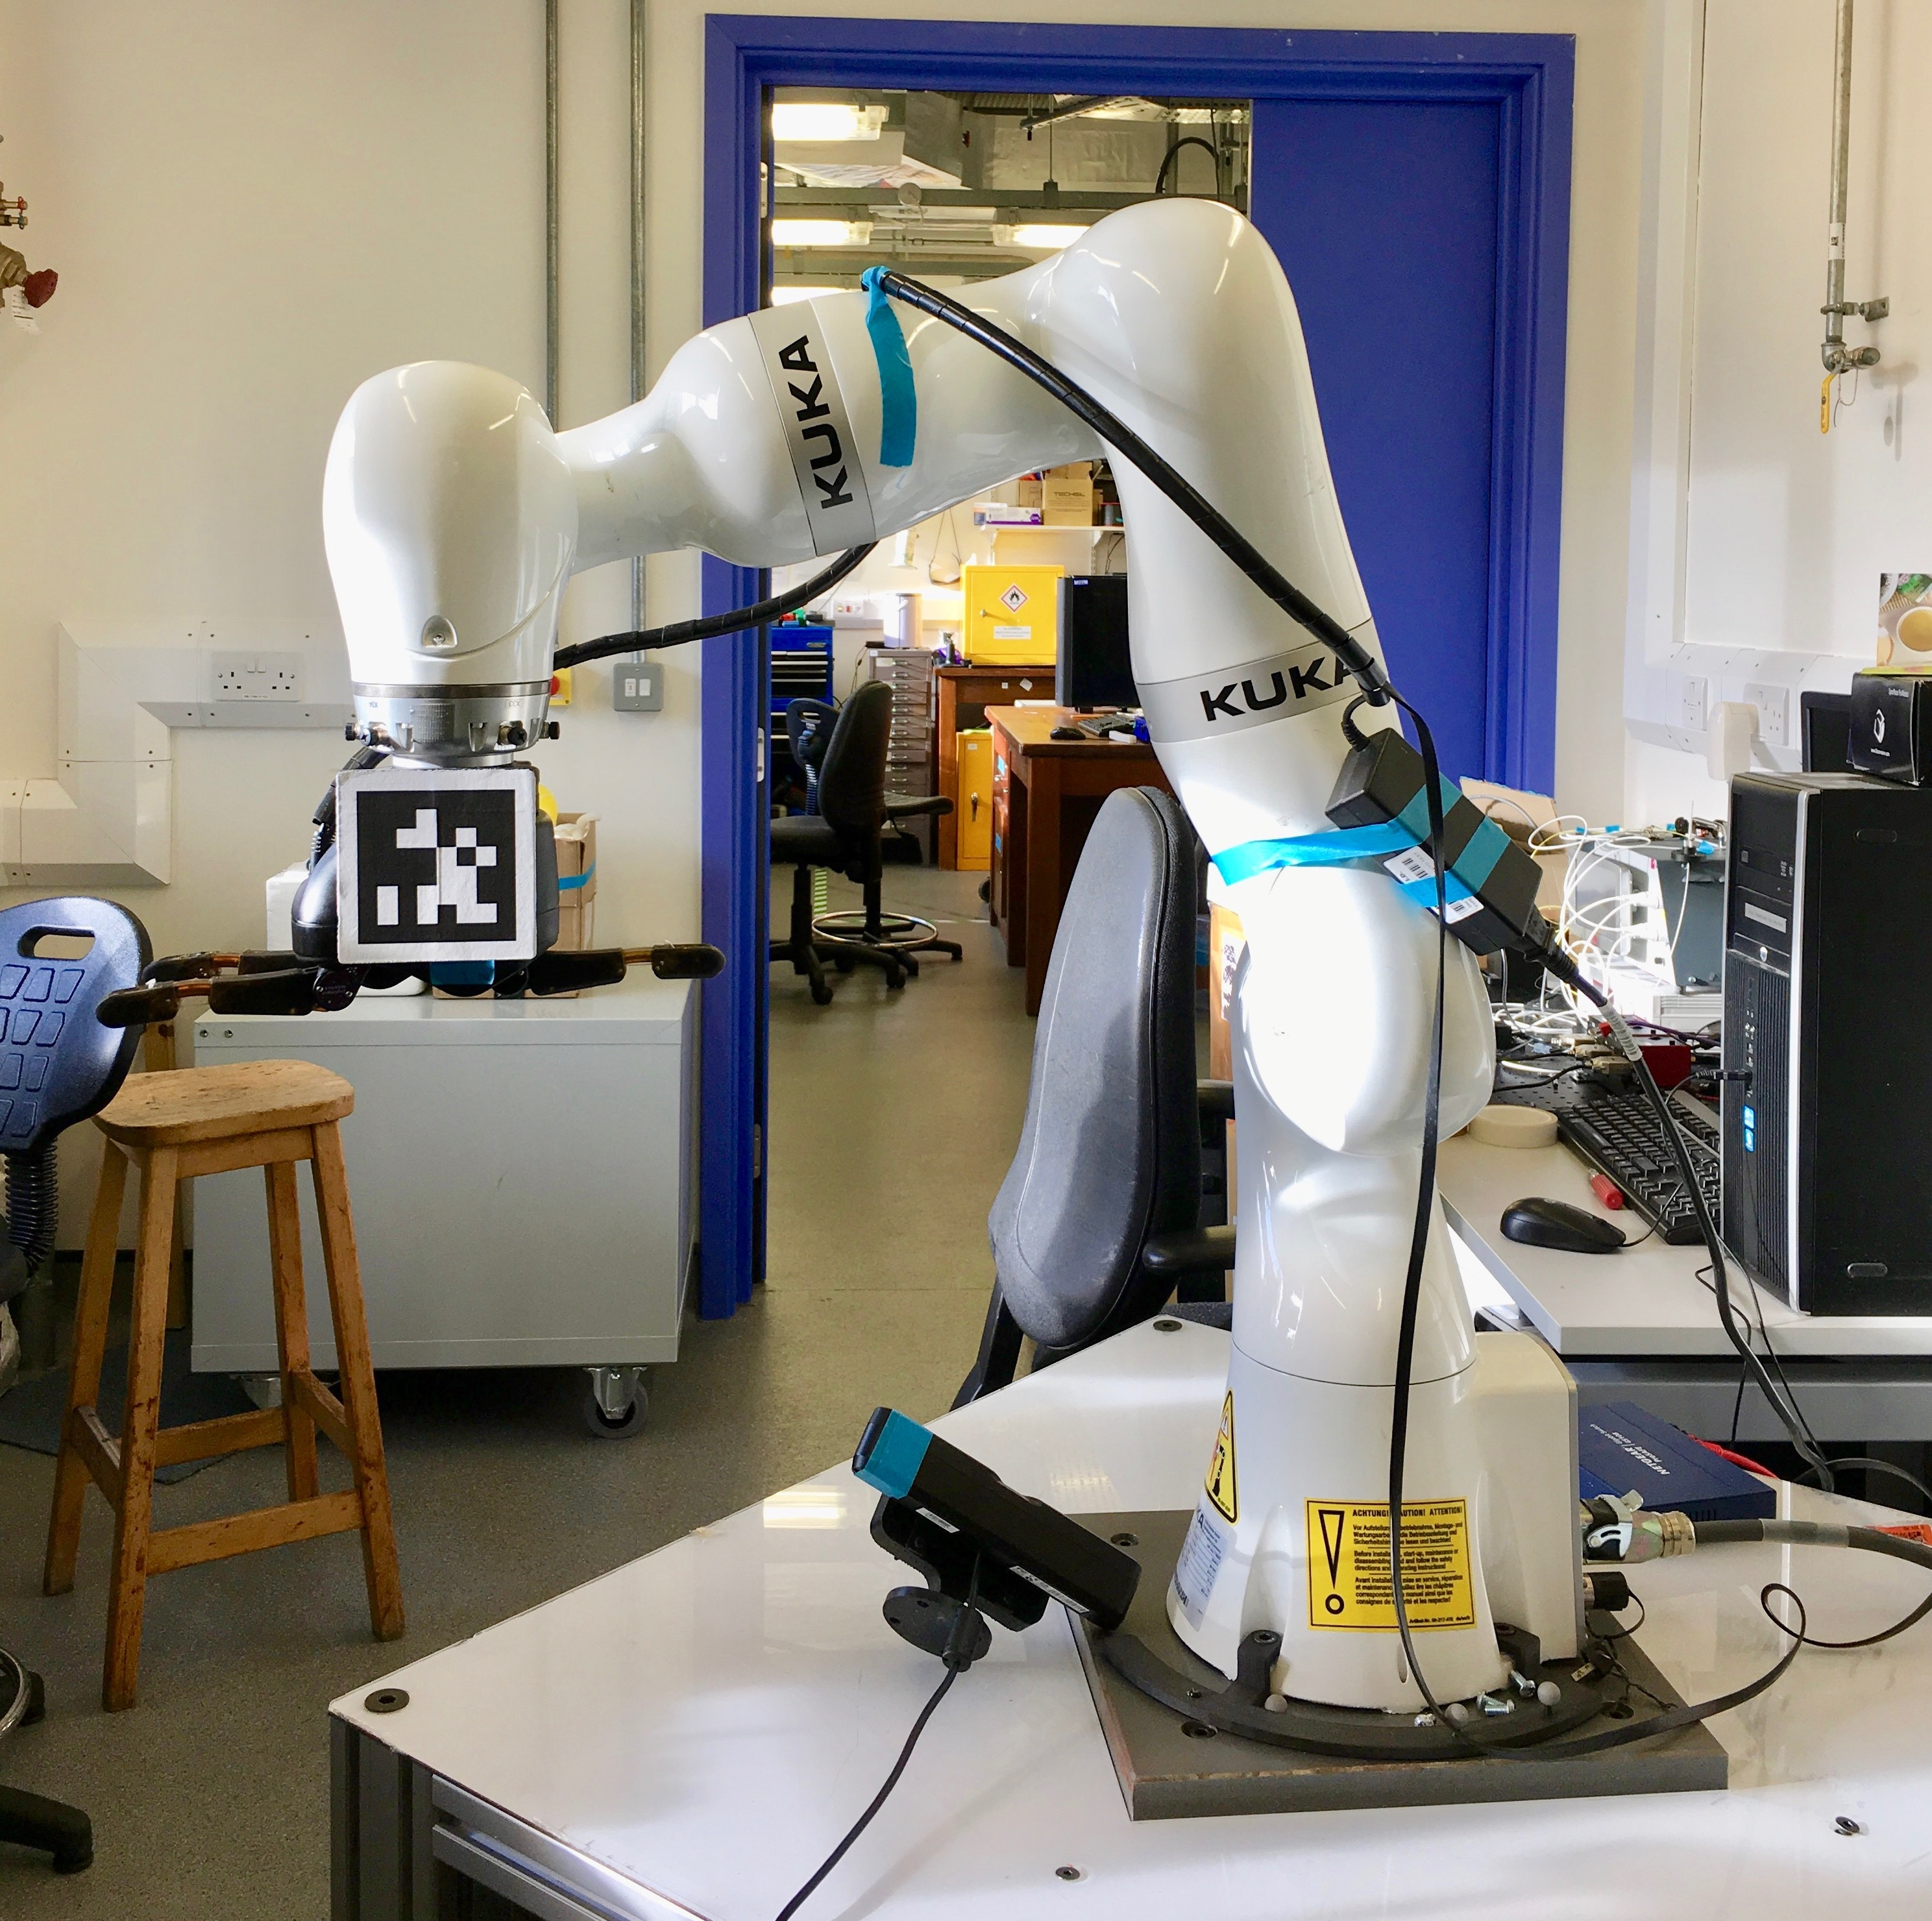
\includegraphics[width=9cm]{figures/case_1}
    \caption{Home position with center line [1,0,0]}
    \label{case_1}
\end{figure}

\begin{figure}[h!]
    \centering
    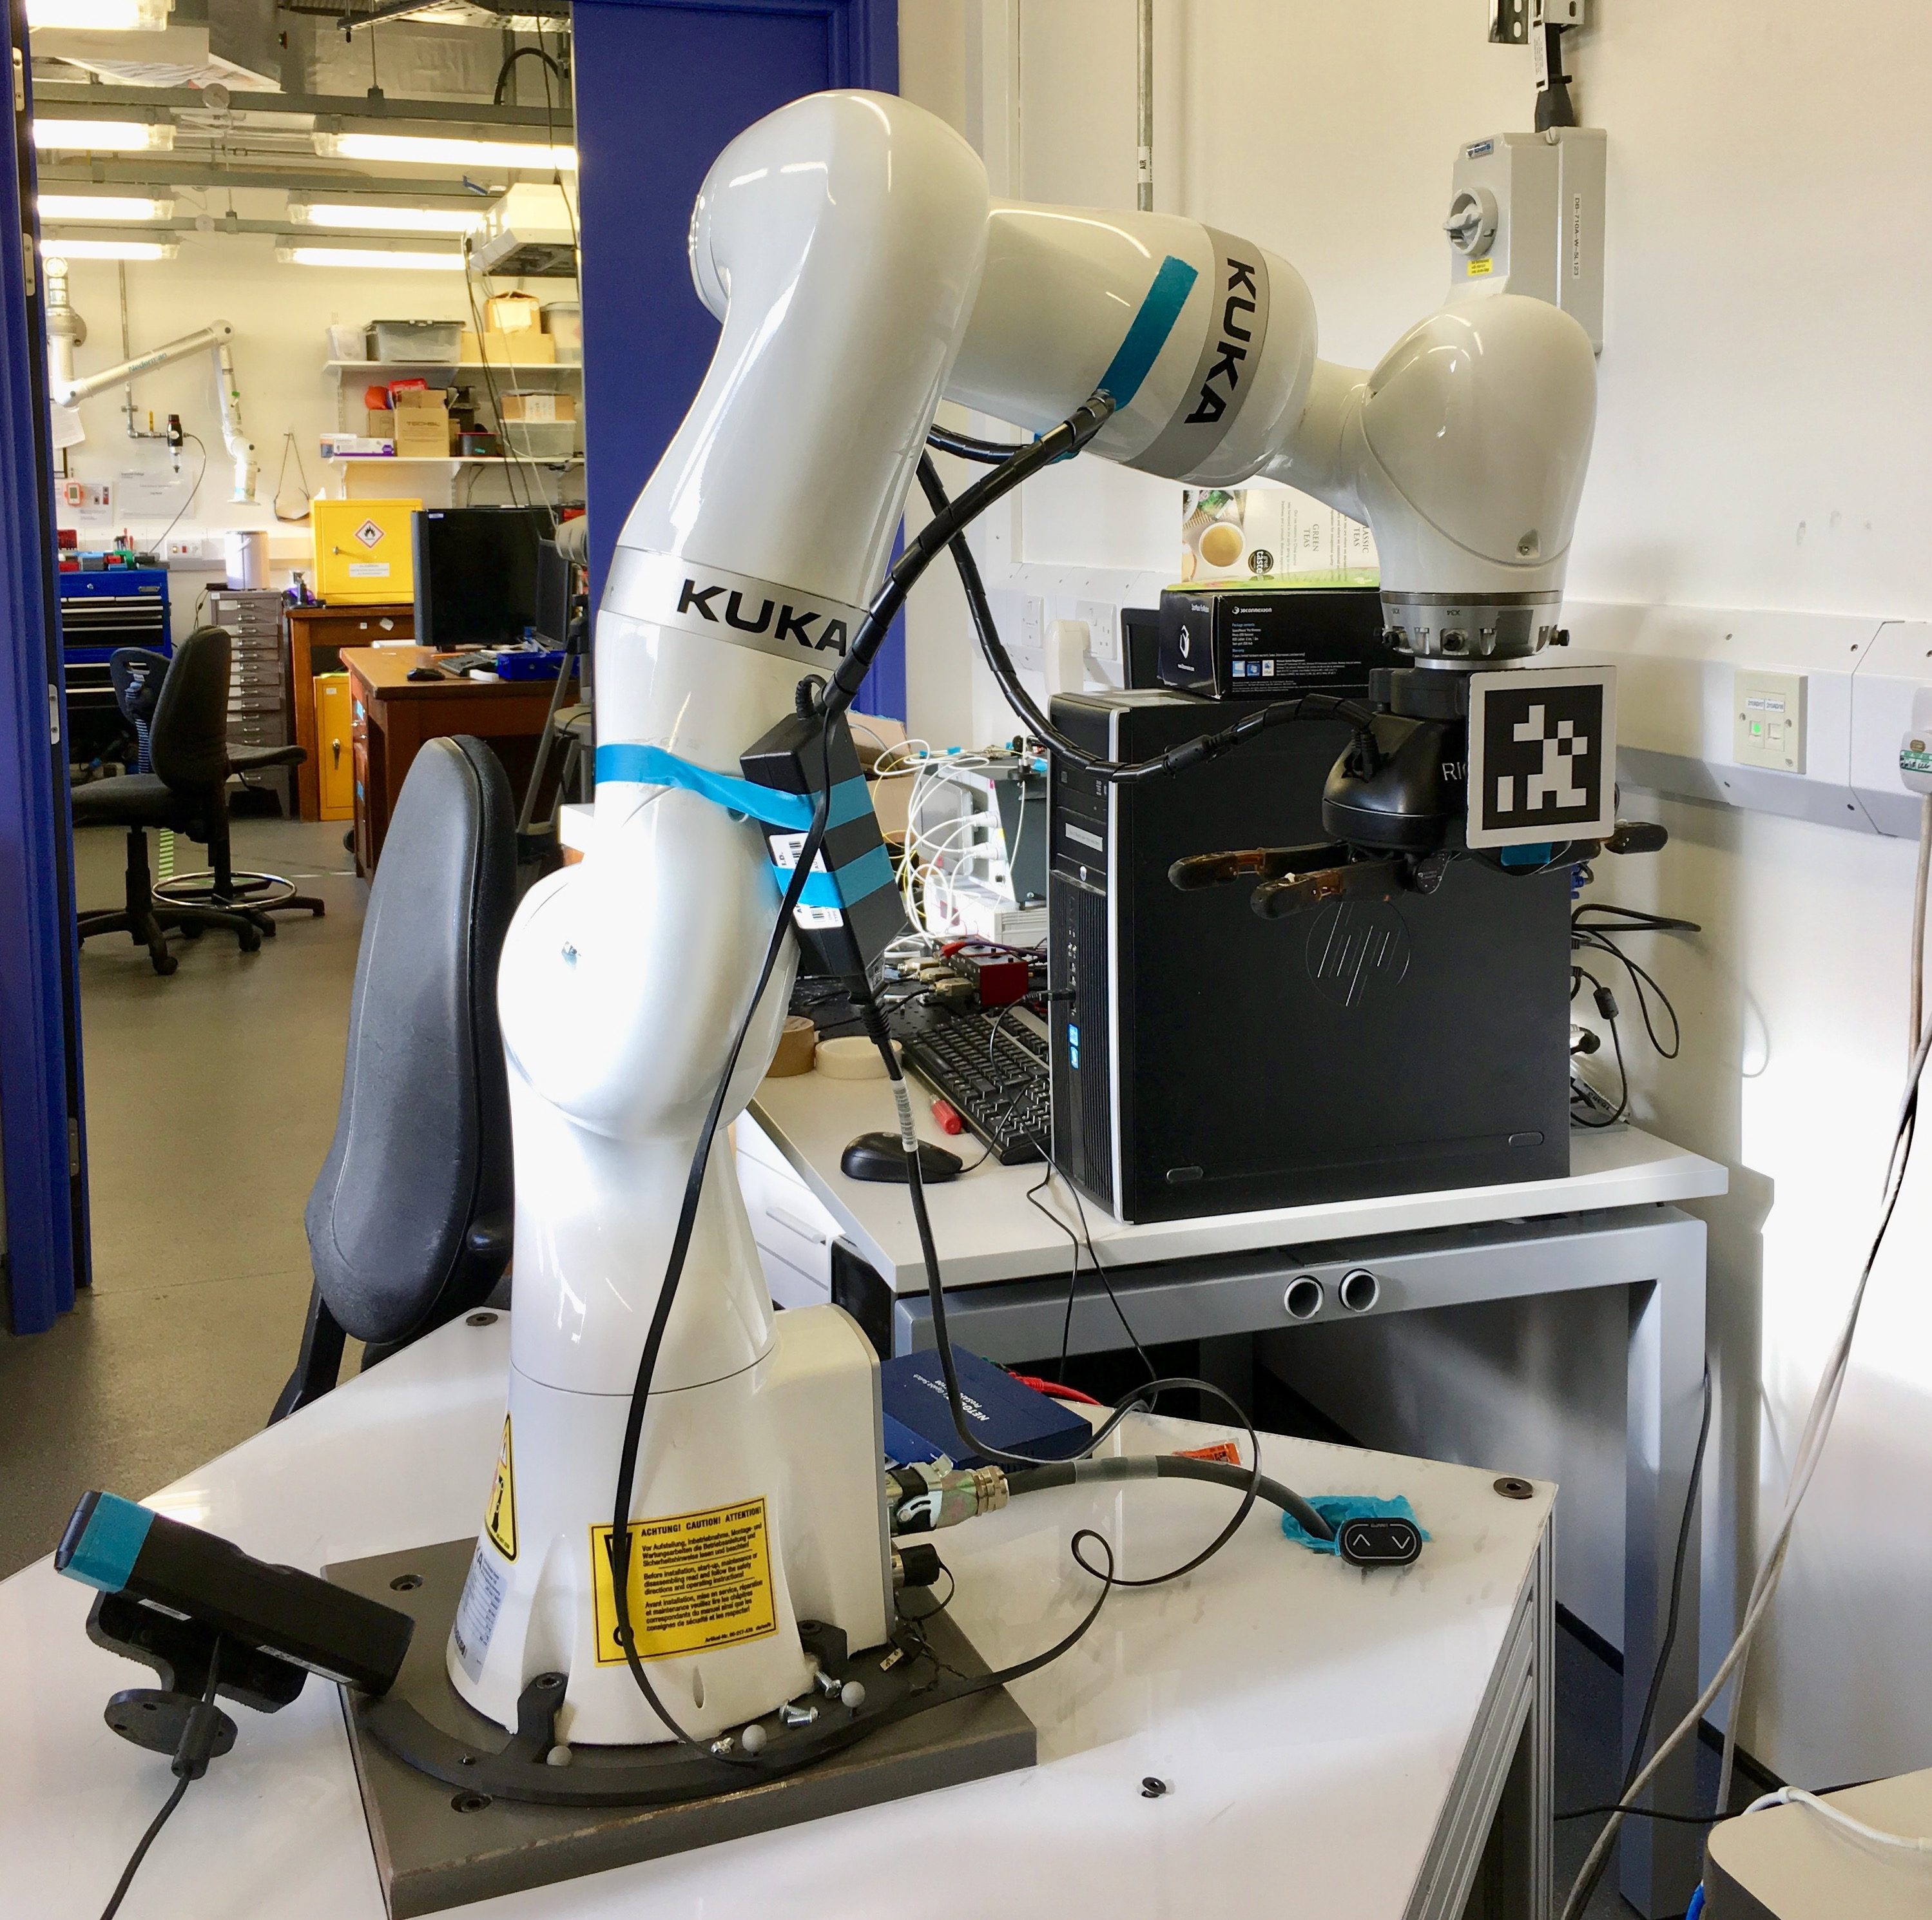
\includegraphics[width=9cm]{figures/case_2}
    \caption{Home position with center line [-1,0,0]}
    \label{case_2}
\end{figure}


\newpage
\subsection{Custom Home Pose}

Seeing that depending on the application (and mounting position of the KUKA) some users may prefer a custom home pose as opposed to the calculated one, the KUKA control nodes offer an option to specify a custom home position in joint space. Simply enter the desired custom home pose in the configuration file under the parameter \texttt{home\_pos}. To use this home pose the \texttt{use\_home\_pos} parameter must be set to \texttt{true}. Otherwise the robot will calculate the home pose as described in subsection \ref{home_calc}. As described earlier the reference point for scaling in the control scripts is the workspace center. Again, the workspace center parameter is set to the tool tip in its home pose.

To find a home position that is suitable for your task consider moving the robot in the desired position using the KUKA touch pad and then simply transferring the displayed joint values to the config file. Please note that it is the operators responsibility to ensure that the tool position in the specified home pose is within the given workspace boundary. Consider adjusting the workspace boundary to fit your custom home position. The script will throw an error if you fail to set a home position inside the boundary. Again, for visualisation the Matlab script \texttt{workspacePlotter.m} can be helpful. See Figure \ref{fig:custom_home} for an example (note the tilted tool transform and the workspace center). 

\begin{figure}[h]
    \centering
    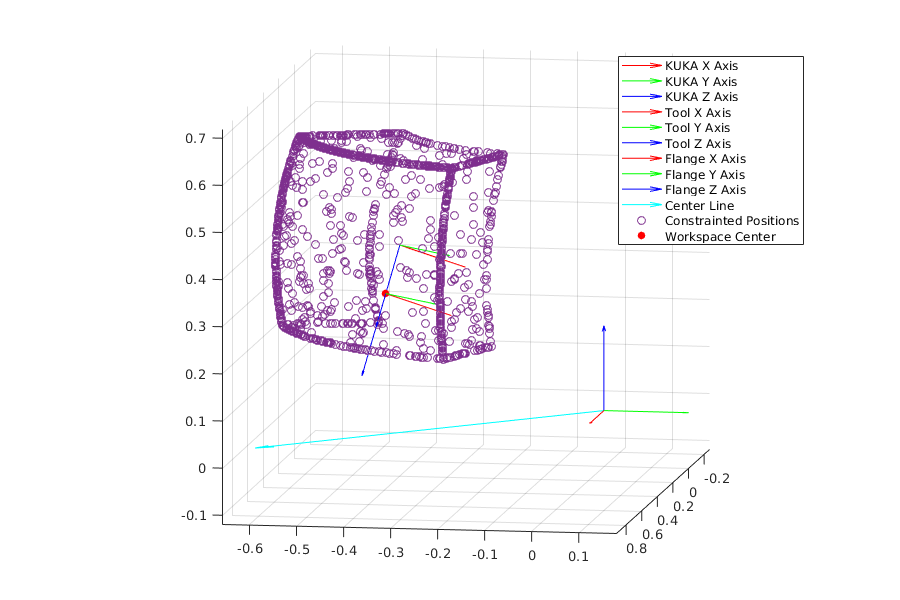
\includegraphics[width=15cm]{figures/ws_custom_home}
    \caption{Plot of workspace custom home position [-45, 20, 0, -100, 0, 40, 0]}
    \label{fig:custom_home}
\end{figure}

\newpage
\subsection{Control Loops}

\begin{algorithm}[H]
 \While{true}{
 \If{exit\_app\_emergency}{return\;}
 \ElseIf{exit\_app}{break\;}
  
 \If{control active}
 {
 \eIf{time out and not at home}{PTP motion to home position\;}
 {get tool transform\;
 scale position\;
 enforce workspace boundary constraints\;
 solve inverse kinematics\;
 check solution validity\;
 \If{movement above threshold}{PTP motion to calculated joint position\;}}}
 \ElseIf{control inactive and not at home}{PTP motion to home position\;}
 publish robot state\;
 }
\caption{PTP control loop}
\label{alg:ptp}
\end{algorithm}

\vspace{0.8cm}
In line 15 of Algorithm \ref{alg:ptp} it is checked whether the individual joint movements to the received pose are bigger than a certain threshold (can be set in the configuration file under parameter \texttt{joints\_thresh}). The idea behind this is that if the \gls{ros} node receives a noisy transform signal the robot does not do \gls{ptp} movements back and forth unless a threshold is surpassed. If every new transform message should be executed the parameter should be set to 0.

\newpage
\begin{algorithm}[H]
 \While{true}{
 \If{exit\_app\_emergency}{return\;}
 \ElseIf{exit\_app}{break\;}
  
 \If{control active}
 {
 \eIf{time out and not at home}{PTP motion to home position\;}
 {get tool transform\;
 scale position\;
 enforce workspace boundary constraints\;
 solve inverse kinematics\;
 check solution validity\;
 \If{not mirroring and at home}{
 \eIf{big jump}{PTP motion to pick-up pose\;}{start real-time control directly\;}
}
 \ElseIf{mirroring}{real-time motion to calculated joint position}}}
 \ElseIf{control inactive and not at home}{PTP motion to home position\;}
 publish robot state\;
 }
\caption{Real-time control loop}
\label{alg:rt}
\end{algorithm}

\vspace{0.8cm}

Line 16 of algorithm \ref{alg:rt} checks whether the movement from the home position to the pick-up pose (i.e. the first tool transform received) surpasses a certain threshold (set to 2 degrees for each joint in the Matlab code). If the threshold is surpassed (e.g. because the input device is not well calibrated with the home tool pose), then a \gls{ptp} movement is done to the pick-up pose, to avoid an abrupt start. Otherwise the node enters real-time mode directly.

In both scripts the timeout is adjustable in the configuration file under parameter \texttt{time\_out}. If no new transformation message is published to the script for longer than the time out allows, the robot will move to its home position. While the time out is not yet expired, it will stay in the pose which was last published to the \gls{ros} network.

\subsection{Running Control Scripts}

This is the standard workflow to use the \gls{ros} control nodes, written in an instructional format. 

\begin{enumerate}
	\item Update configuration file (\texttt{kuka\_params\_rt.yaml} or \texttt{kuka\_params\_ptp.yaml}) to your needs. Consider visualising the workspace definition first using the \texttt{workspacePlotter.m}.
	\item Make sure the defined workspace is clear and no obstacles are within it.
 	\item Boot the robot, establish ethernet connection and start MatlabToolboxServer application on KUKA robot controller in automatic mode.
 	\item Upload workspace configuration parameters to \gls{ros} parameter server. You can use the included launch files named \texttt{kuka\_params\_rt.launch} or \texttt{kuka\_params\_ptp.launch} for this, depending on which workspace you want to upload.
	\item Run Matlab nodes for the control method you need (either \texttt{realTimeController.m} or \texttt{ptpController.m}).
	\item Robot now moves to calculated (or otherwise specified) home pose.
	\item Activate the control mode via a \gls{ros} service call to \texttt{kuka/kuka\_control} or via the GUI. 
	\item Robot starts to listen to the \texttt{tf/} topic.
	\item Make sure you publish the right tool transformation depending on if the tool's X axis points towards or away from the base. Refer to Figure \ref{fig:home_position} for more information on this.
	\item Publish on the \texttt{tf/} topic. You need to provide the transform from \texttt{kuka/base\_frame} to \texttt{kuka/flange\_frame/desired}. Make sure every message contains an updated time tag. 
	\item Robot moves to specified tool transforms.
	\item If you activate the gripper control (using the \texttt{kuka/gripper\_control} service or the GUI) a corresponding boolean flag is published on the \texttt{kuka/gripper\_control} topic.
	\item Switch the KUKA control off with the service \texttt{kuka/kuka\_control} or the \gls{gui} when you do not need it anymore. The robot moves home. You can reactivate it anytime. 
	\item When done, exit the application with the \texttt{kuka/exit\_app} service or the GUI. Robot moves to zero position and terminates connection to KUKA robot.
	\end{enumerate}

\newpage
You should pay attention to these things while using the \gls{ros} \gls{kst} interface.

\begin{itemize}
	\item If you are in real-time mode and the first transform you send is far away from the home position (in joint space) the robot will perform a \gls{ptp} movement to the pick-up position. From this point onwards all further transforms are executed in real-time mode. This should avoid abrupt starts if the initial tool transform you send does not lie in the close vicinity of the home configuration (e.g. due to miscalibration). However, if the first transform you send is sufficiently close to the tool home transform the robot will execute in right real-time mode straight away.
	\item For the real-time control mode a \textbf{frame rate of at least 50 Hz} is recommended. For the \gls{ptp} mode the frame rate can be lower. However, make sure that the frame rate is high enough such that timeout threshold is not reached. If the Matlab \gls{ros} node does not receive any new \texttt{tf/} messages for longer than the threshold allows, it will move to its home position.
	\item This is especially relevant in real-time mode: it is your responsibility to do \textbf{adequate filtering} of the transform message before sending the transforms to the control node. A sequence of good transform messages for the real-time node should form a smooth trajectory. For example, this can be achieved by simple averaging filters or more complex Kalman filters. The KUKA control node simply executes the received transform messages and does not filter.
	\item If in your task it is cumbersome to Figure out the full transformation from the KUKA base frame to the desired tool frame you could control the robot relative to its home pose. The home pose of both the flange and the tool in the base frame are constantly published to the \gls{ros} tf tree. These fixed transforms are called \texttt{kuka/flange\_frame/home} and \texttt{kuka/tool\_frame/home} respectively.
	\item The \texttt{ptpController.m} always moves with the relative velocity specified in the parameter \texttt{velocity\_ptp} of the \gls{ptp} configuration file. 
	\item The \texttt{realTimeController.m} moves to its home position (beginning) and zero position (end) with \texttt{velocity\_ptp\_slow}. All \gls{ptp} movements in the meantime (i.e. back to home position when no more new data is incoming or when KUKA control stopped) are executed with relative velocity \texttt{velocity\_ptp\_fast}.
	\item In both the real-time mode and the \gls{ptp} mode, the \gls{ros} node will disregard any incoming transform messages that are sent while the robot is executing a motion. It will only listen to the most recent transform message on the tf tree, once its previous movement was executed.
	\item All movements are scaled around the tool tip in the home position if your scaling factor does not equal to 1. Remember: using the calculated home pose, this corresponds to the geometrical workspace center (see Figure \ref{fig:ws_center}). Using a custom home pose the movement will be scaled around the tool position in the given home position.
	\item If you wish to deactivate all workspace constraints in a control script look for the function call of \texttt{getConstrainedPosition} and delete it. Note: deactivating the workspace boundary might be dangerous. The robot can move freely and will execute any transform you send unless it is not executable by the robot.
	\end{itemize}

\section{Leap Motion}

\subsection{Leap Configuration File}

The configuration file is called \texttt{leap\_params.yaml} and is part of the \texttt{leap\_kuka} \gls{ros} package.

\begin{table}[h]
\centering
\begin{tabular}{lll}
\textbf{Paramater Name} & \textbf{Default}    & \textbf{Note}                                   \\
z\_clearance            & 0.15                & remaining hand offset when lower z limit reached \\
box\_dimensions         & {[}0.2, 0.2, 0.2{]} & dimensions of interaction box                   \\
buffer\_size            & 10                  & size of averaging buffer                        \\
start\_tol\_pitch       & 20                  & tolerance for hand pitch at pick-up             \\
start\_tol\_roll        & 20                  & tolerance for hand roll at pick-up              \\
run\_tol\_yaw           & 25                  & tolerance for hand yaw while running            \\
run\_tol\_pitch         & 25                  & tolerance for hand pitch while running          \\
run\_tol\_roll          & 25                  & tolerance for hand roll while running           \\
min\_confidence         & 0.05                & do not use data if below minimum confidence    
\end{tabular}
\caption{Leap Motion configuration parameters}
\label{tab:leap_params}
\end{table}

\newpage
\subsection{Coordinate Systems}

In this software the hand coordinate system is defined as follows (see Figure \ref{fig:hand_coosy}). The coordinate system definition is exactly the same for right and left hand (see Figure \ref{fig:two_hands_coosy}).

\begin{enumerate}
	\item \textbf{X axis}: hand direction vector as defined by Leap Motion 
	\item \textbf{Y axis}: completes right handed coordinate system
	\item \textbf{Z axis}: palm normal vector as defined by Leap Motion 
\end{enumerate}

\begin{figure}[h]
    \centering
    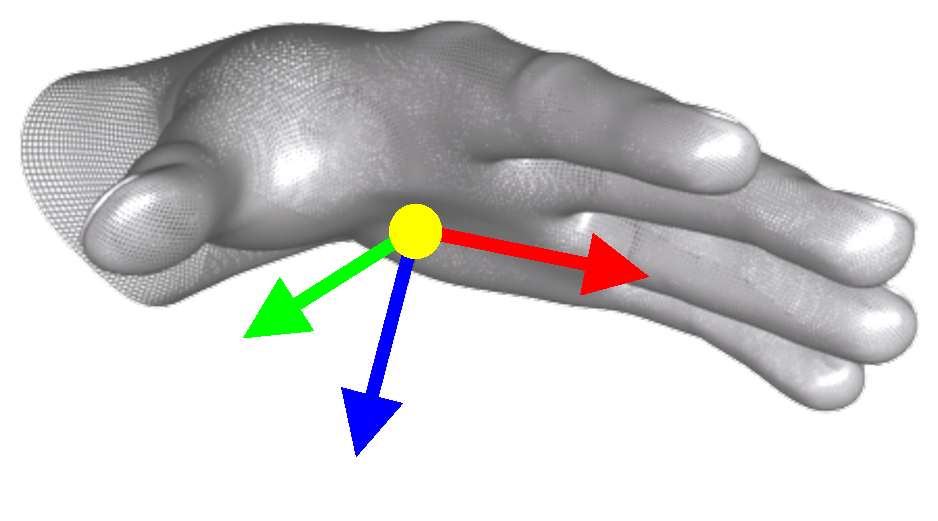
\includegraphics[width=9cm]{images/hand}
    \caption{Hand coordinate system \cite{LeapImages}}
    \label{fig:hand_coosy}
\end{figure}

\begin{figure}[h]
    \centering
    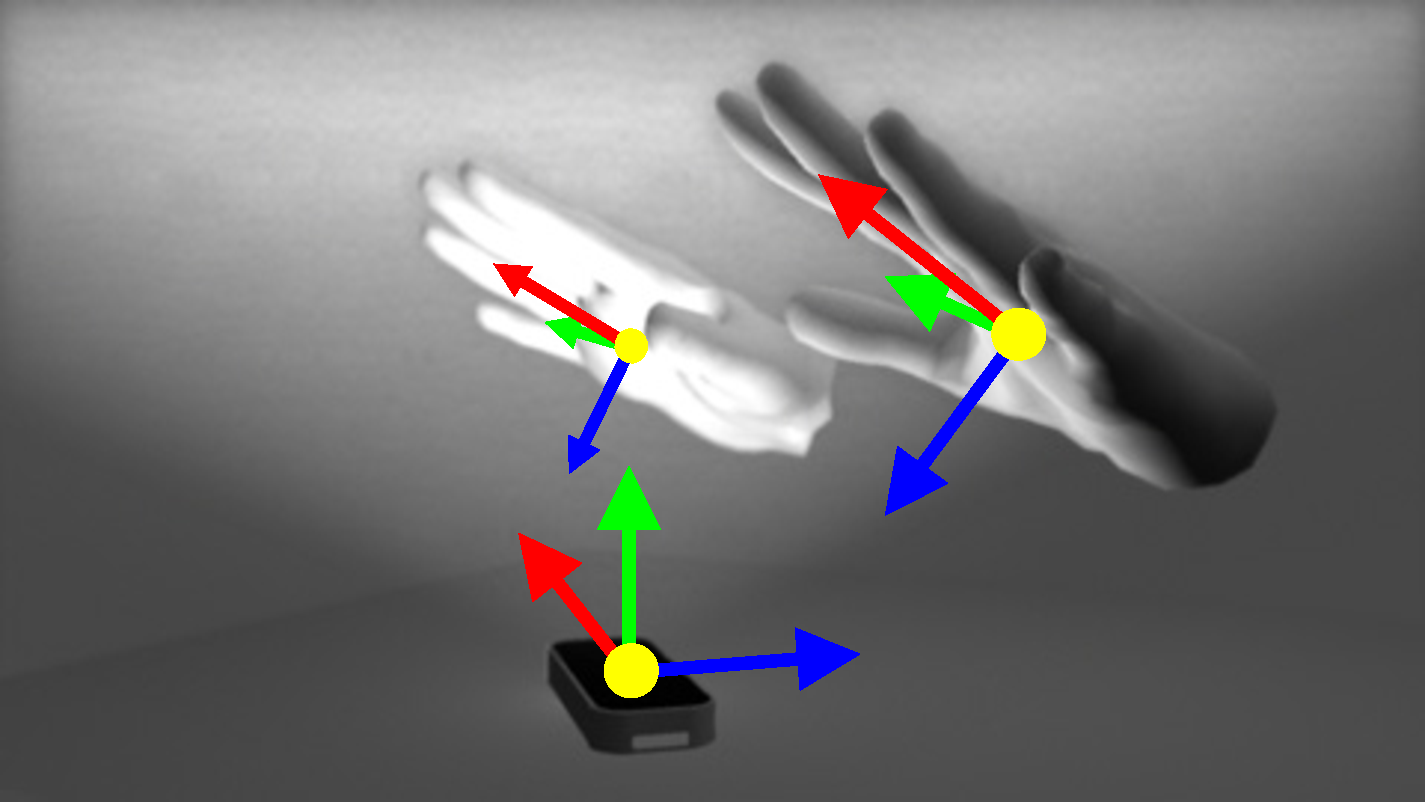
\includegraphics[width=9cm]{images/two_hands}
    \caption{Coordinate systems of left hand right hand \cite{LeapImages}}
    \label{fig:two_hands_coosy}
\end{figure}

Figure \ref{fig:leap_coosy} shows how the leap motion reference frame is defined. It is important to note that the image in Figure \ref{fig:leap_coosy} is only correct if users put in their first hand with finger tips pointing towards the green LED. If the option "Auto-orient Tracking" in the settings of the LeapControlPanel is activated the Leap Motion flips its Z axis depending on which side the user is entering the tracking volume, such that the Z axis always points towards the user's finger tips. This was taken account during the development of the Leap KUKA node.

\begin{figure}[h]
    \centering
    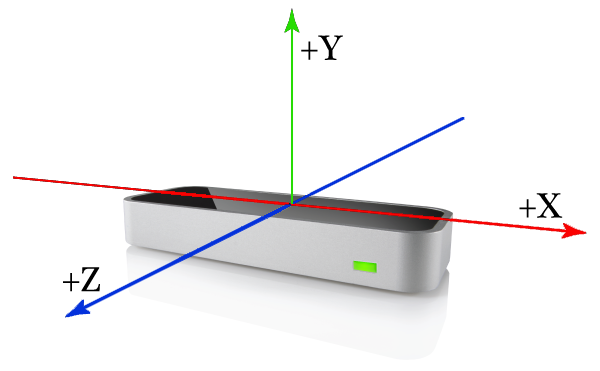
\includegraphics[width=9cm]{images/leap_coosy}
    \caption{Leap Motion coordinate system \cite{LeapImages}}
    \label{fig:leap_coosy}
\end{figure}

\subsection{Coordinate Transformations}

A major part of this project is the investigation of teleoperation techniques using gesture tracking. The Leap Motion tracking device is used to control the KUKA real-time \gls{ros} node presented earlier. Figure \ref{fig:overview_coosys} shows an overview of the general idea of the \gls{ros} node: The Leap Motion is virtually placed in some convenient location and orientation such that the position and orientation of the detected hand received in the Leap Motion reference frame can be directly mapped to the desired tool pose in the KUKA base frame.

\begin{figure}[h]
    \centering
    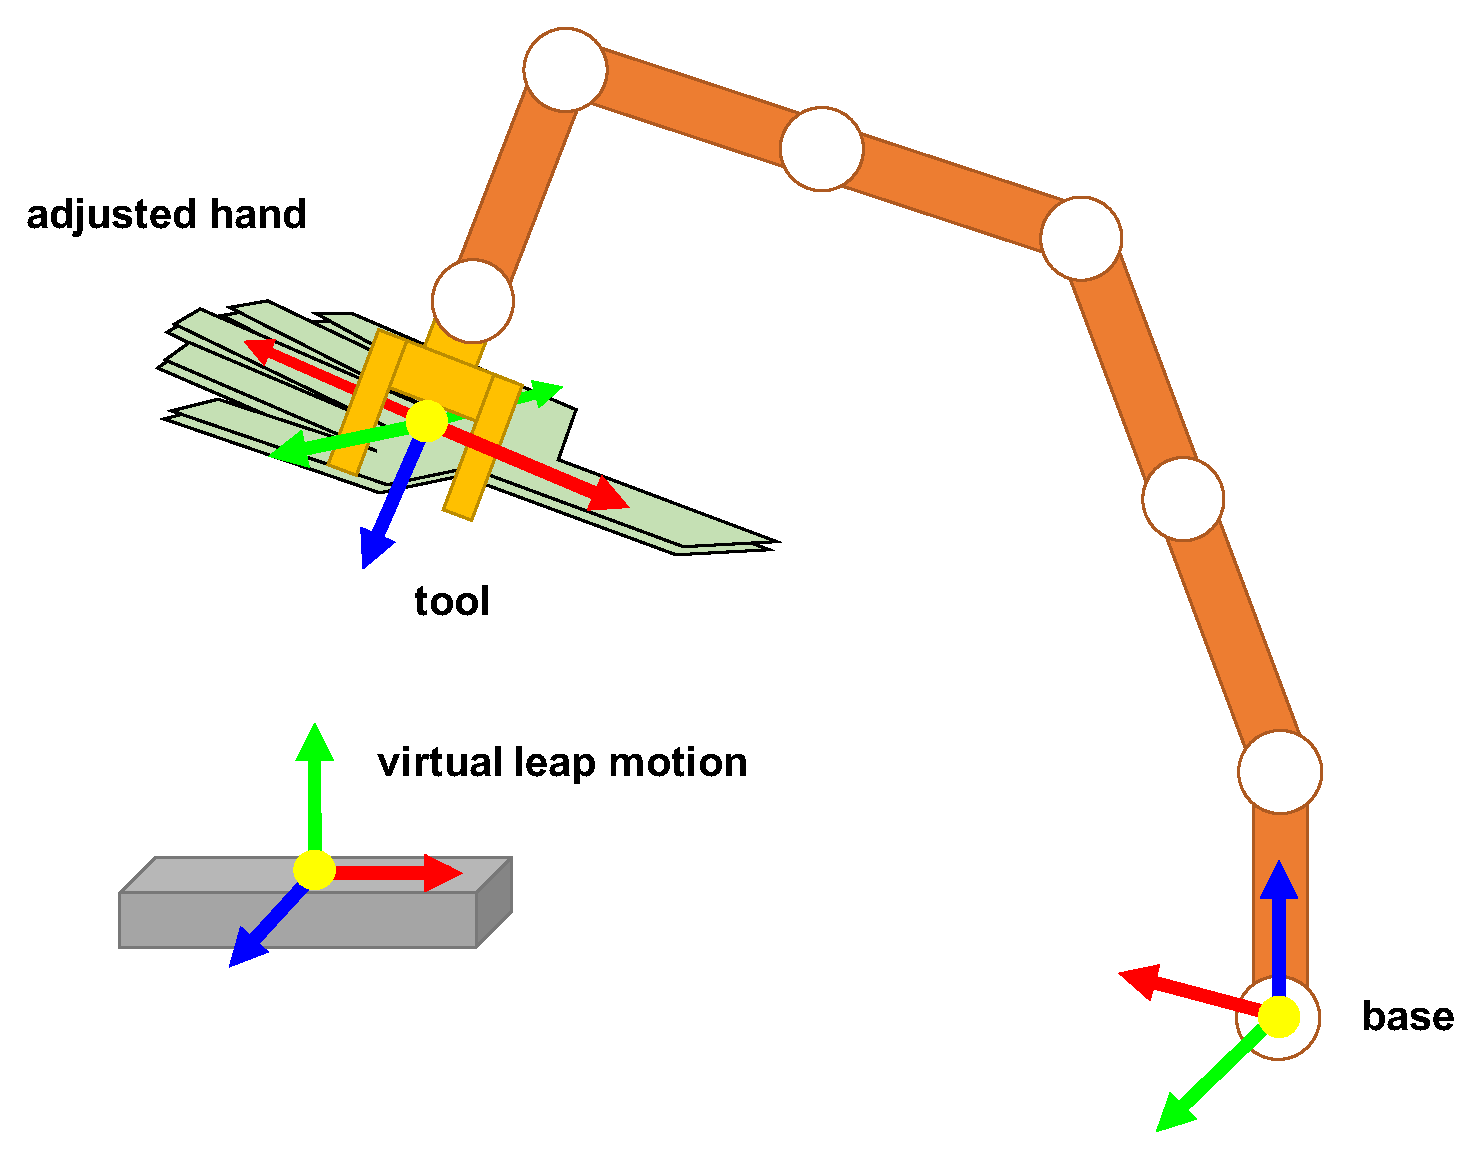
\includegraphics[width=10.5cm]{images/coosy_overview}
    \caption{Coordinate transformations overview}
    \label{fig:overview_coosys}
\end{figure}

\newpage
Table \ref{tab:transforms} shows a list of all transformations published by the \texttt{leap\_kuka} node. The following paragraphs explain how each of the transformations is obtained.

\begin{table}[h]
\centering
\begin{tabular}{ll}
\textbf{From}               & \textbf{To}                 \\
kuka/base\_frame            & leap\_motion/virtual\_frame \\
leap\_motion/virtual\_frame & hand/frame                  \\
leap\_motion/virtual\_frame & kuka/tool\_frame/desired    \\
leap\_motion/virtual\_frame & kuka/flange\_frame/desired 
\end{tabular}
\caption{Transformations published by leap\_kuka node}
\label{tab:transforms}
\end{table}

\subsubsection{leap\_motion/virtual\_frame}

The calculation of the transform from KUKA base to virtual Leap Motion relies on two ideas. The position of the Leap Motion lies directly below the workspace center (i.e. tool home position). The Z offset from the workspace center is the distance between workspace center and lower Z limit plus the Leap Motion clearance parameter. A graphical overview of this is given in Figure \ref{fig:leap_pos}. As the workspace center must be known before the virtual Leap Motion position can be calculated it must be uploaded to the \gls{ros} parameter server before launching the Leap KUKA node. This is done by the control scripts presented earlier.

\begin{figure}[h]
    \centering
    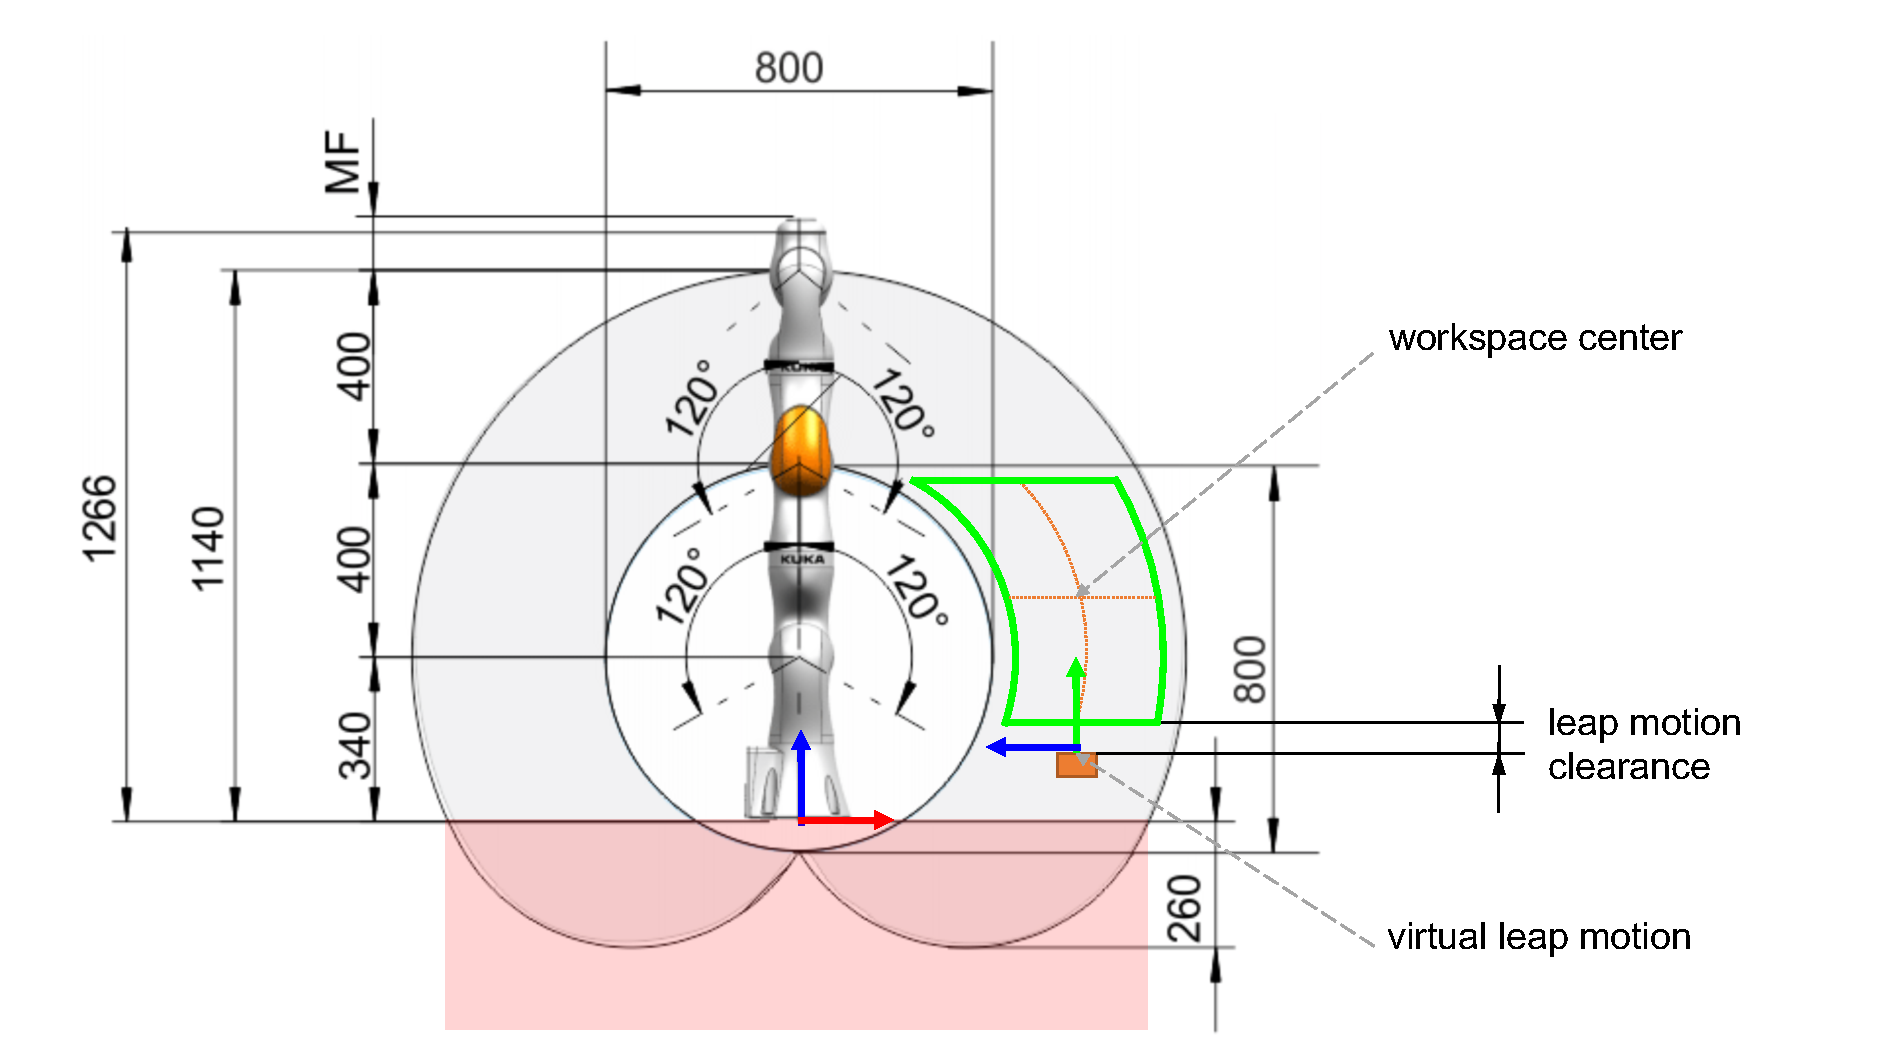
\includegraphics[width=13cm]{images/leap_ws_side}
    \caption{Position of Leap Motion in KUKA base frame}
    \label{fig:leap_pos}
\end{figure}

Furthermore, the orientation of the Leap Motion is determined by two constraints. Firstly, the Leap Motion Y axis must be parallel to the KUKA Z axis. Secondly, the Leap Motion must be rotated around its Y axis such that the XY components of the first detected hand's direction vector points in same direction as the center line. This means that the hand frame measured by the Leap Motion and the fixed hand frame in Figure \ref{fig:leap_transform} must line up. Therefore it is completely arbitrary with which yaw angle the user's hand approaches as the Leap Motion will always be rotated around its Y axis to fulfil the second constraint. Please note that users should actually align their hands with the robots center line when using the system. Otherwise the control of the robotic rig might feel unintuitive.

\begin{figure}[h]
    \centering
    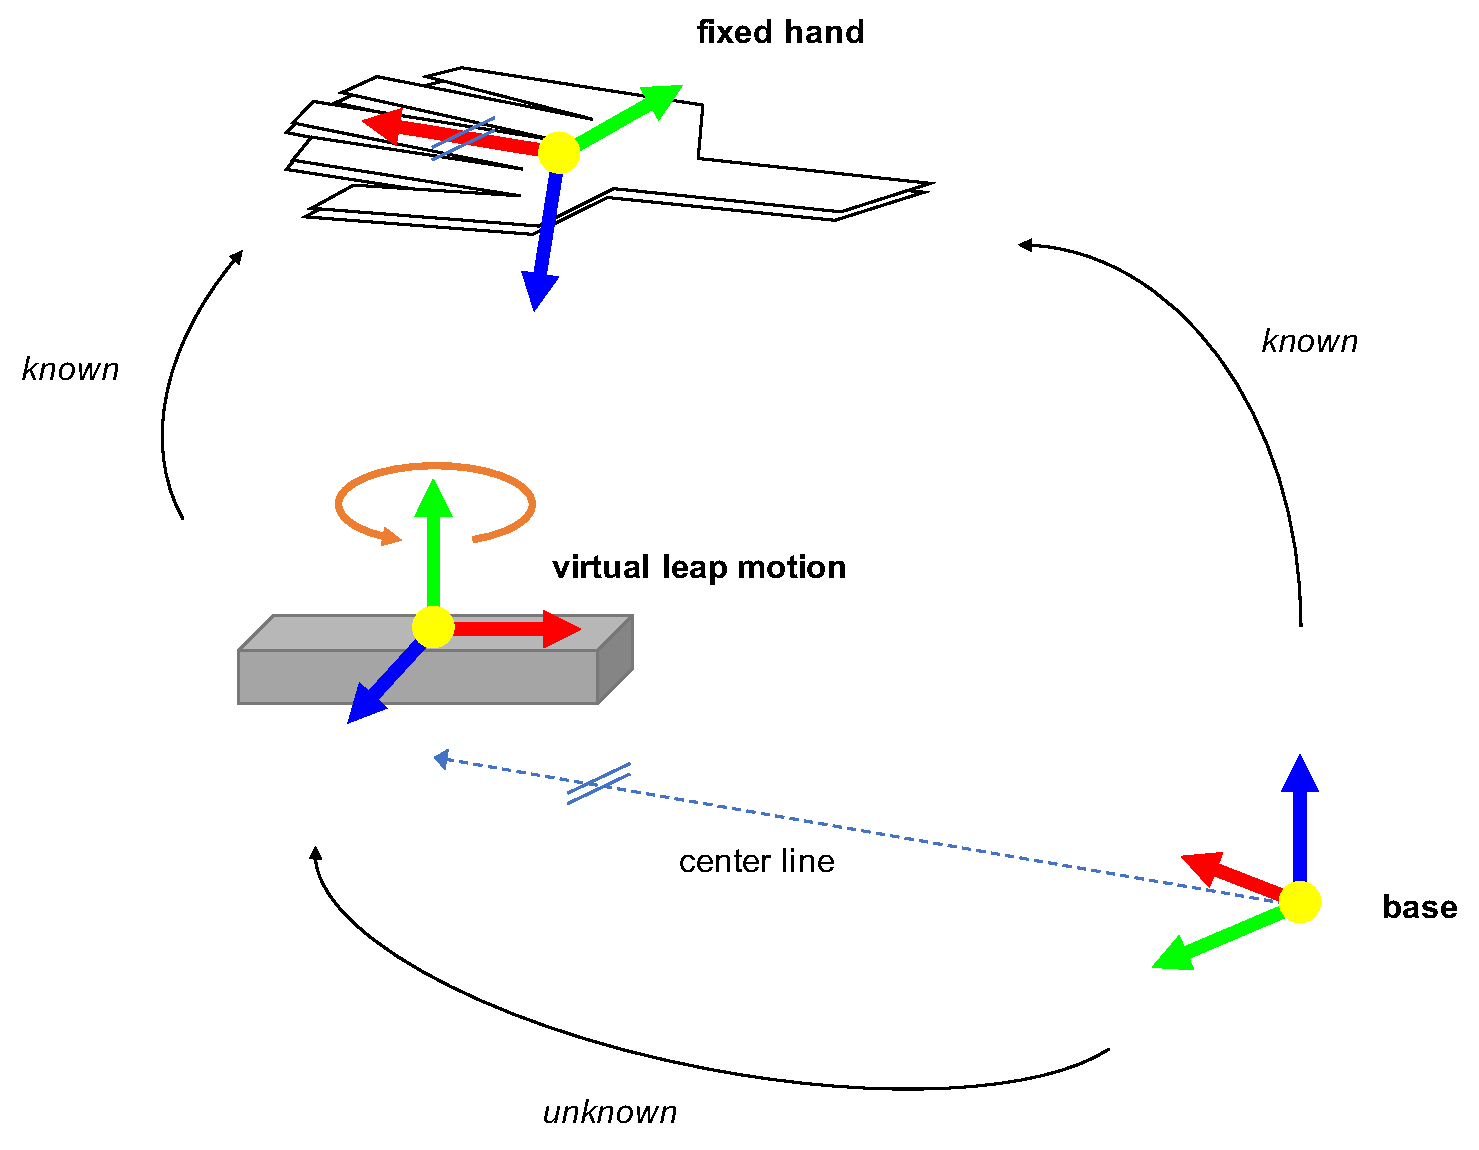
\includegraphics[width=14cm]{images/leap_transform}
    \caption{Transformation to virtual Leap Motion}
    \label{fig:leap_transform}
\end{figure}

\subsubsection{hand/frame}

The hand frame is simply the transform determined from data which the Leap Motion collects about the hand. The transform is computed from the hand's X, Y and Z axes (refer to Figure \ref{fig:hand_coosy}) and the palm's center position. 

\newpage
\subsubsection{kuka/tool\_frame/desired}

As mentioned earlier the measured hand frame should be mapped to the desired tool frame. The position of the desired tool frame always equals the position of the measured hand.

The orientation includes a further step. Since the measured hand might exceed the running tolerances specified in the Leap Motion configuration file an adjusted hand frame is introduced (which is not published to the tf tree). The adjusted hand frame equals the measured hand frame if yaw pitch and roll are within the running tolerances. However, if the measured hand exceeds the allowed yaw, pitch or roll the hand's orientation must be adjusted as depicted in Figure \ref{fig:hand_transform}. Yaw, pitch and roll are measured around the fixed hand frame. If any of the yaw, pitch or roll constraints are exceeded the adjusted hand's rotation is simply the measured hand's rotation with adjusted values (which if exceed correspond to the maximum allowed rotation and otherwise represent the measured hand's rotation). 

\begin{figure}[h]
    \centering
    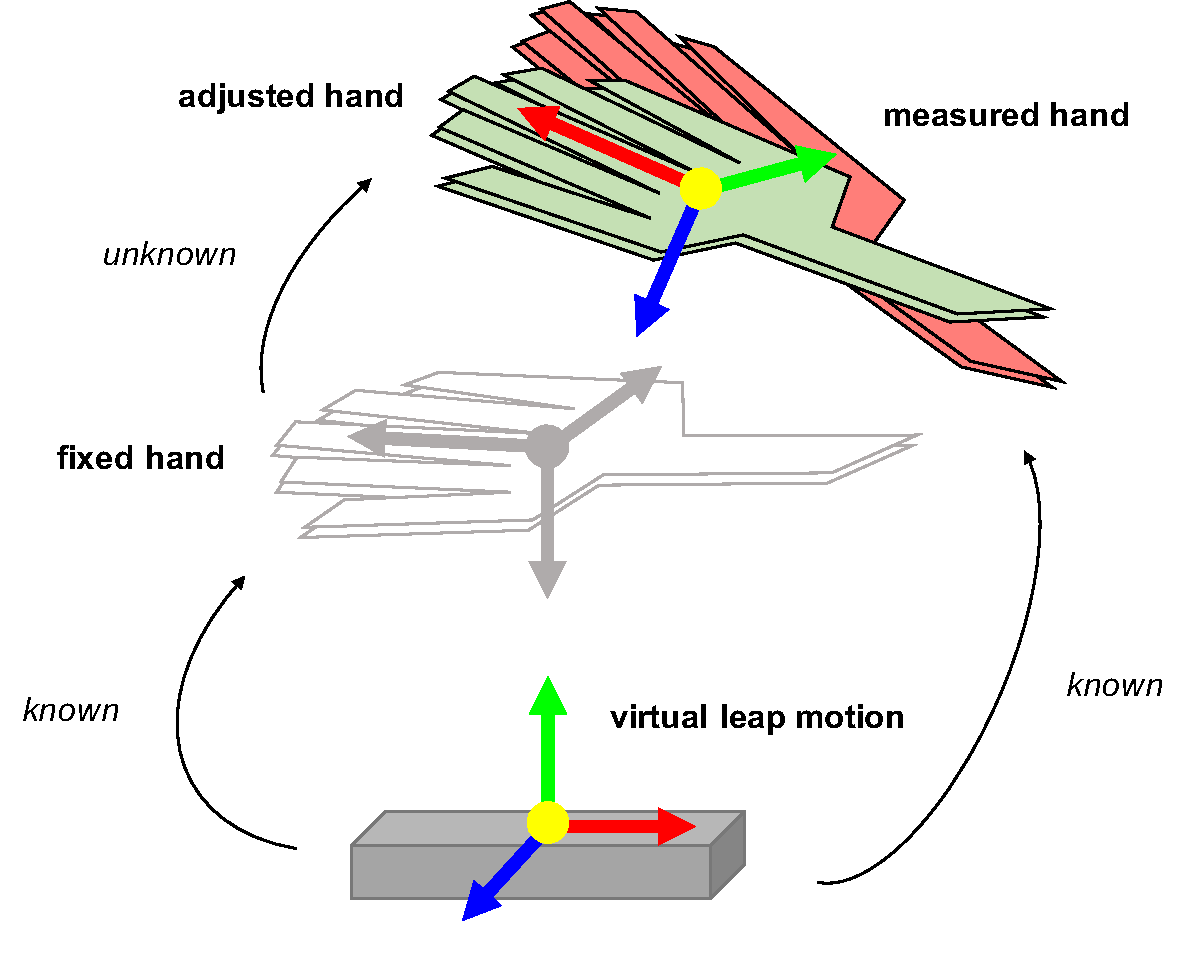
\includegraphics[width=11cm]{images/hand_transform}
    \caption{Transformation to desired KUKA tool pose}
    \label{fig:hand_transform}
\end{figure}

It is assumed that the automatic home pose calculation feature from section \ref{home_calc} is used. Depending on where the center line points the home tool orientation with respect to the base can look different (refer to Figure \ref{fig:home_position}). Depending on where the center line points the adjusted hand's frame is rotated 180 degrees around its Z axis and then published to the tf tree. 

\subsubsection{kuka/flange\_frame/desired}

The desired flange frame is simply the tool frame translated by the specified tool length along its negative z axis. It is not used to control the KUKA robot, but still published for completeness. 

Figure \ref{fig:leap_rviz} shows a final overview of the frames published by the Leap KUKA node (except the flange frame for better visibility). Note how the rotation of the \texttt{hand/frame} exceeds one of the rotational constraints and the \texttt{kuka/tool\_frame/desired} frame is rotated less. The position of both frames coincides.

\begin{figure}[h]
    \centering
    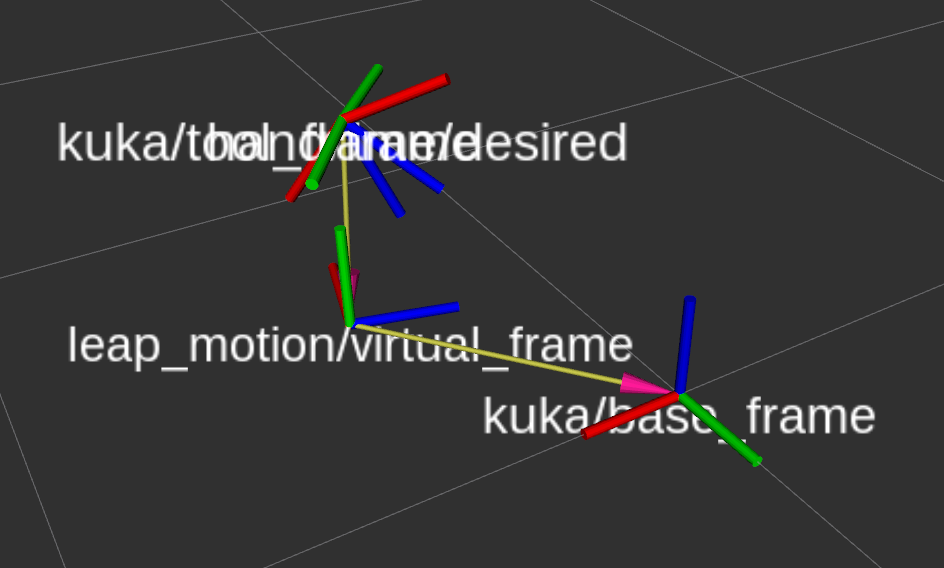
\includegraphics[width=11cm]{figures/leap_frames_rviz}
    \caption{Frames published by leap\_kuka node viewed in RViz}
    \label{fig:leap_rviz}
\end{figure}

Things users should pay attention to when using the \texttt{leap\_kuka} \gls{ros} node. 
\begin{itemize}
	\item To start publishing the desired tool frame put a hand inside a virtual interaction cube above the Leap Motion. Keep hand horizontal (within specified tolerances). Leap Motion orientation on table does not matter. Node uses a FIFO queue for averaging of data. Once enough data for the averaging process is collected node publishes the desired tool transform. 
	\item The system does not distinguish between left or right hands. You can use either hand.
	\item If two hands are detected the system always regards the hand which has been visible the longest.
	\item Switch "Auto-orient Tracking" in LeapControlPanel settings on to take leverage of full capability of \gls{ros} node. If switched off, the Leap Motion only recognizes hands coming in from one lateral side.
	\item If for debugging purposes (never for control!) you would like to run the Leap KUKA node independently you can do so using the \texttt{leap\_kuka\_debug.launch} launch file. Note that in order to make the node run independently this file uploads default values for the \texttt{center\_line} and  \texttt{ws\_center} arguments - hence only use it for debugging and visualisation. 
\end{itemize}

\chapter{Robotic Hand Node} \label{hand}
\section{General}

The ReFlex Takktile robotic hand by RightHand Robotics is a 4 degree of freedom force sensitive robotic gripper. It can be conveniently controlled through the \gls{ros} driver which is included in the \texttt{modules} folder. Before attempting to control the robotic hand make sure that the networking setup (see section \ref{networking}) was completed successfully. Below is the workflow for controlling the robotic hand.

\begin{enumerate}
\item Power robotic hand.
\item Establish valid ethernet connection.
\item Type \texttt{roslaunch reflex reflex\_takktile.launch} in a terminal to launch the robotic hand's \gls{ros} driver.
\item Calibrate the hand before using it (especially before first usage) by calling the services \texttt{reflex\_takktile/calibrate\_fingers} and \texttt{reflex\_takktile/calibrate\_tactile}. \newline The calibration results will be stored in a directory inside the hand \gls{ros} driver. Make sure the hand is in an adequate zero position (i.e. fingers stretched out) before calibrating. 
\item Publish to the right closure angles to the topic \texttt{reflex\_takktile/radian\_hand\_command}. The message must be of type RadianServoCommands and consists of four numbers in the order [index, middle, thumb, spread]. The opened hand command corresponds to [0, 0, 0, 0] and a closed hand command would correspond to [2, 2, 1.8, 0].
\end{enumerate}

\section{Leap Motion}



The Python script \texttt{leap\_hand.py} forms a \gls{ros} node to control the robotic hand intuitively using the Leap Motion gesture tracking device. The control node calculates four angles from vectors that it constructs starting from the palm center position. In Figure \ref{fig:human_flexion} alpha represents the index finger flexion, beta the middle finger flexion and gamma the thumb flexion angle. Angle delta (not in figure) represents the spread between index and middle finger. 

\newpage
\begin{figure}[h]
    \centering
    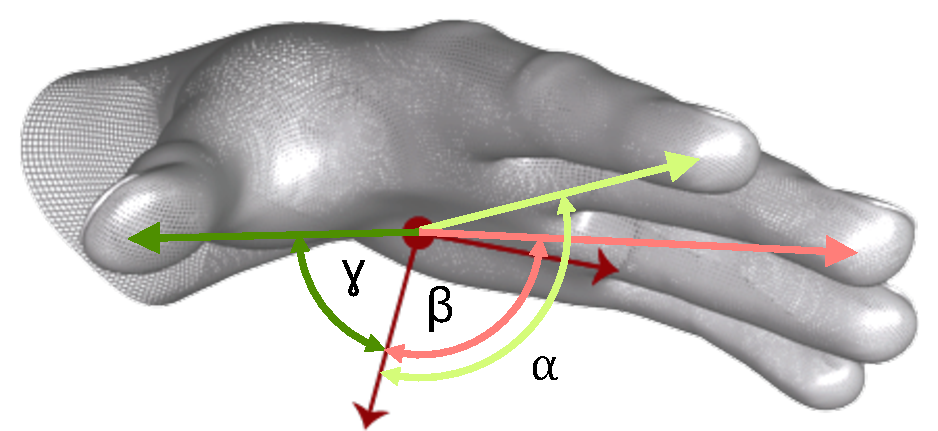
\includegraphics[width=9cm]{images/hand_angles}
    \caption{Human flexion angles \cite{LeapHand}}
    \label{fig:human_flexion}
\end{figure}

\begin{enumerate}
	\item \textbf{alpha}: angle between palm normal and vector to index finger tip
	\item \textbf{beta}: angle between palm normal and vector to middle finger tip
	\item \textbf{gamma}: angle between palm normal and vector to thumb tip
	\item \textbf{delta}: angle between vectors from palm center to center of intermediate bones
\end{enumerate}

Once the \texttt{leap\_hand.py} node calculated the human flexion angles it maps the measured angles to the minimum and maximum specified flexion angles of the robotic hand. This allows for smooth opening of the individual fingers (as opposed to simple open/close movements). If no hand is detected the robotic hand flexion equals is set to the open pose. The  array of robotic hand flexion angles is published to the \texttt{reflex\_takktile/radian\_hand\_command} topic. The script works with either hand.


\chapter{Tips and Tricks}
\section{Leap Rig Demo}

These are short instructions for users that would like to show the demo of Leap Motion control of the robotic hand and the KUKA robot. These instructions may repeat information previously presented in the report.

\begin{enumerate}
	\item Adjust configuration files \texttt{kuka\_params\_rt.yaml} and \texttt{leap\_params.yaml} to your needs (especially consider reading through subsection \ref{ws_def} on the workspace definition).
	\item Setup system as shown in Figure \ref{fig:hardware_architecture} (robot, hand and computer connected via ethernet through a switch and Leap Motion connected to computer using USB)
	\item Start KUKA Robot with green toggle on robot controller. Wait for it to boot.
	\item On the KUKA touch pad, press "Applications" in the top left and click on the application "MatlabToolboxServer".
	\item Mount and power the Robotic Hand. Make sure that its fingers are in a flat (i.e. opened) position as this will be its zero position.
	\item Establish network connection to KUKA and robotic hand by clicking on the devices in "Ethernet Networks" in the top right corner. If you click on "kuka" or "hand" it should say "Connection Established".
	\item Make sure the defined robot workspace is clear.
	\item Run the application on the KUKA touch panel by clicking green arrow pointing to the right (button is on the left of the touch pad). Make sure that you are in automatic mode. This can be changed by twisting the black knob in the top of the touch panel in a horizontal position. Change the mode to AUT if necessary and turn it back.
	\item Navigate to the \texttt{leap\_rig/shell} folder and launch both shell scripts in listing \ref{shell}. Note that if your workspace is not called \texttt{catkin\_ws} you must adjust the path to your workspace name in the \texttt{run\_leap\_control.sh} script.
	\item Once the robot moved to its home position, activate KUKA control and robotic hand control by \gls{ros} service calls or with the "ROS Control" toggles in the Matlab GUI.
	\item Put hands inside a virtual interaction cube which sits above the Leap Motion. Keep hand horizontal. Leap Motion orientation on table does not matter. Once enough data for the averaging process is collected the robot will start mirroring the hand motions.
	\item Switch the KUKA control off with the service \texttt{kuka/kuka\_control} or the \gls{gui} when you do not need it anymore. The robot moves home. You can reactivate it anytime. 
	\item When done, exit the application with the \texttt{kuka/exit\_app} service or the GUI. Robot moves to zero position and terminates connection to KUKA robot.
\end{enumerate}

\begin{lstlisting}[language=bash, caption={Launching Leap Rig demo}, label={shell}]
cd ~/catkin_ws/src/leap_rig/shell
./run_leapd.sh
./run_leap_control.sh
\end{lstlisting}


Please consider this when running the demo.
\begin{itemize}
	\item Consider running the Diagnostic Visualiser when clicking on the LeapControlPanel (green rectangle in top left corner). It gives a nice demo of the Leap Motion system to people who are not yet familiar with it. 
	\item When someone is controlling the robot always have hand on the KUKA emergency stop button.
	\item Should you leave the robot unsupervised press the emergency stop button or switch the robot off.
	\item You might want to increase the buffer size of the averaging queue of the Leap KUKA node in its configuration file. This will make the robot less responsive and lead to a smoother trajectory. 
	\item Before switching the KUKA "ROS Control" on explain, that users have to put their hand inside a virtual cube above the Leap Motion to "pick up" the robot. Their hand has should be horizontal and still when put inside the interaction box. Further, their hand and forearm should be parallel to the robot arm to ensure intuitive control.
	\item Before letting others control the robot, let them get a feeling for the system by only letting them control the Robotic Hand first. Explain, that only the thumb, index and middle finger are used to control the hand. The other fingers should be as straight as possible. The reason for this is that if users make a fist, the Leap Motion will produce a noisy signal for hand position, direction and normal from which the tool transformation is calculated.
\end{itemize}

\newpage
The following is a summary of safety features of the software setup.

\begin{itemize}
	\item Robot performs a safety stop if it senses a cartesian torque of 25Nm or higher.
	\item The maximum end effector velocity is set to 800mm/s. Robot performs safety stop if this velocity is exceeded. The maximum torque and velocity are specified in the KUKA project which is synchronised to the controller (view KUKA Sunrise Workbench documentation).
	\item To start the Leap Motion control of the robot, the operator has to actively press the toggle "ROS Control". Only if this button is active, the system will pick up the data from the hand inside the cube and start mirroring (i.e., real-time control).
	\item To operate the robot users have to put their hands inside a virtual cube directly above the Leap Motion. This ensures that the system is starting tracking in an area that is well perceived by the Leap Motion and signal noise is kept to a minimum.
	\item At startup users have to put their hands in a horizontal position. Tolerances are specified in the Leap Motion configuration file. This ensures that the robot tool moves to a reasonable position and orientation in a controlled manner.
	\item Very fast hand movements are compensated for in averaging process.
	\item At all times during mirroring, the software limits yaw, pitch and roll to a specified value in the Leap Motion configuration file.
	\item Emergency button in Matlab \gls{gui} instantly stops script. Don't press unless in an emergency. Use "Exit Application" for safe exit and return to zero position.
	\item All positions that would be sent to the robot are checked. If they are not inside the workspace, they are clipped to the workspace boundary.
	\item If any position is "very" infeasible (i.e., negative KUKA z axis or in negative center line direction) the program throws an error and terminates.
\end{itemize}

\newpage
\section{Troubleshooting}

\begin{itemize}
	\item If the robot stops while mirroring your hand movements, you probably exceeded the maximum end effector velocity (800mm/s). Pressing the "run" button (green triangle pointing to the right) should continue the session. You might want to increase the averaging buffer size to make the robot's movements less responsive. 
	\item "Error using \texttt{KST/net\_establishConnection}": If this error shows in Matlab, check the ethernet cables and make sure that you are actually connected to the robot in "Ethernet Networks" in the top right corner. If you press "kuka", your computer should say "Connection Established". Also make sure the MatlabToolboxServer is running on the robot controller. It shuts down again after a while if no connection request is made. 
	\item "No KRC connection possible": If this error message shows on the KUKA touch panel after booting, try rebooting the robot. Ideally, unplug the robots ethernet cable from the switch before booting. The error should then be resolved.
	\item "Could not attach tool to the flange": You get this error message from the KUKA Sunrise Toolbox if the previous connection to the robot was not successfully shut down (happens if  "Emergency Stop" in Matlab is performed). Reboot the robot.
	\item Java Bind Exception: If you get this message on the robot panel, this means your previous connection to the robot did not terminate successfully. Reboot the robot.
	\item Robot does not start mirroring: Check if the toggle "ROS Control" in the KUKA Panel of the \gls{gui} is activated and your hand is in a horizontal position and inside the interaction box. Also make sure that the Leap daemon is running. You could use the Diagnostic Visualizer (right click on green rectangle, LeapControlPanel needs to be running) to check if the Leap Motion is actually detecting a hand. If it does not, but it should, try relaunching the Leap daemon.
	\item No Connection to robotic hand possible: Make sure the power cable is plugged into the Robotic Hand. Unfortunately it does not always sit in place firmly. As with the KUKA make sure that your ethernet cable is correctly plugged in and you have a valid connection under "Ethernet Networks".
	\item If robot detected resistant force: The robot will pause the application running on the KUKA controller. You should be able to press the green button and unpause the motion. If that does not work or the robot ran into more problems, you might need to restart it.
	\item Other unexpected behaviour: Check the command window in Matlab, you might find valuable information there.
\end{itemize}

\newpage
\section{Leap Motion Details}

\begin{figure}[h!]
    \centering
    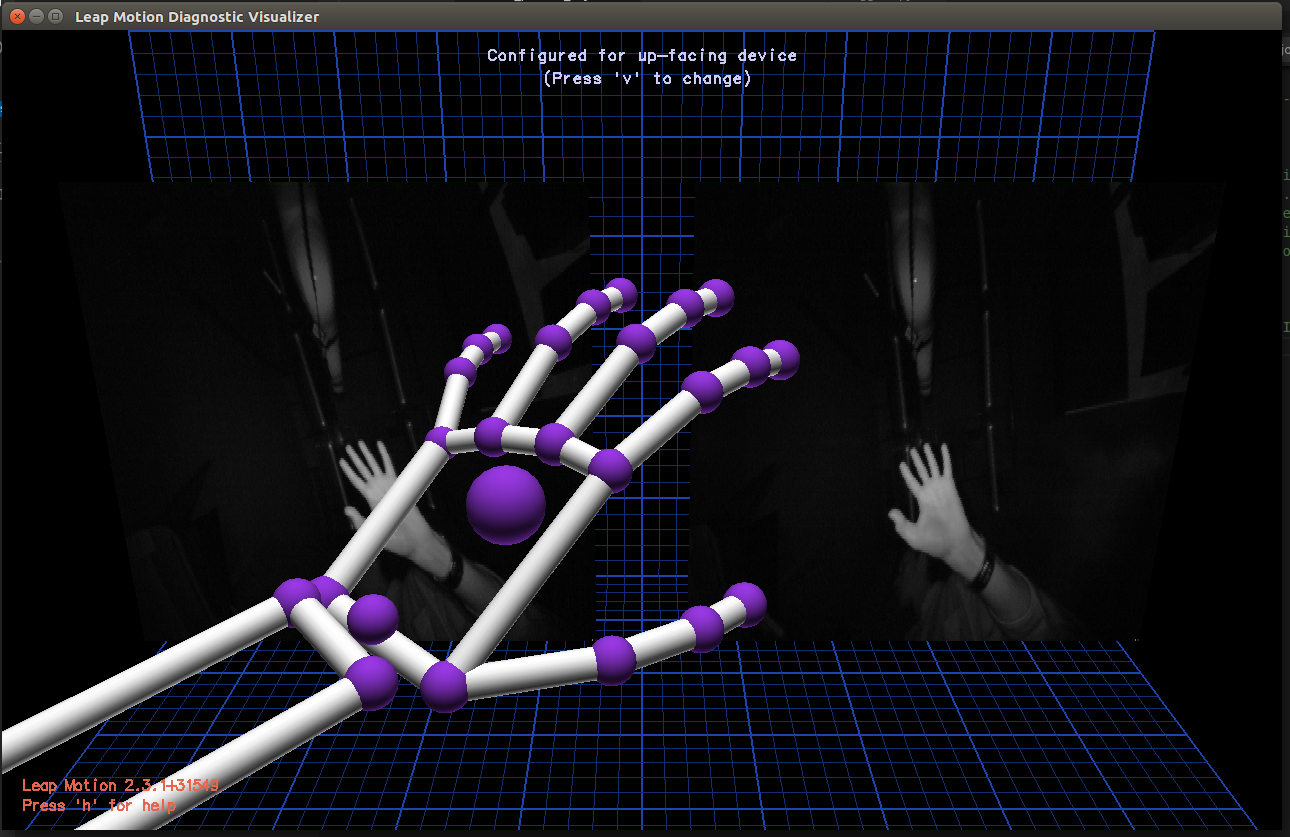
\includegraphics[width=\textwidth]{figures/leap}
    \caption{Leap Motion diagnostic visualizer}
\end{figure}

\begin{figure}[h!]
    \centering
    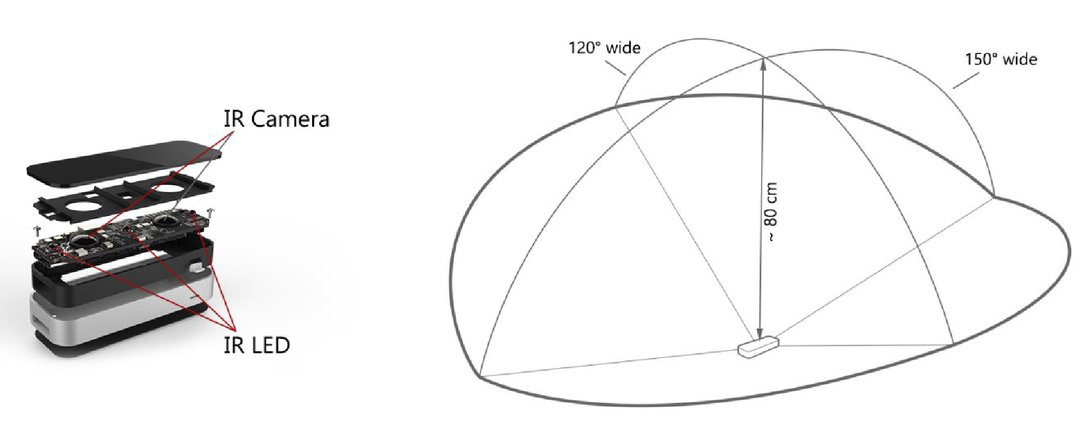
\includegraphics[width=\textwidth]{images/leap}
    \caption{Leap Motion workspace \cite{Wozniak}}
\end{figure}

\newpage
\section{ROS Commands}
\begin{lstlisting}[language=bash, caption={Useful \gls{ros} commands}]
rosclean purge
rosparam list
rosservice list
rostopic list 
rosrun tf view_frames
rostopic echo topic_name
roscore
rqt_image_view
rosrun rviz rviz
catkin build
roslaunch pkg_name file_name.launch
\end{lstlisting}


\chapter{Vision}
\section{Virtual Reality}

To start \gls{vr}  support simply plug in the \gls{rgbd} camera and the Oculus. Make sure that the Oculus is detected as an external display by launching the nvidia-settings utility from the command line if necessary. The Ubuntu home screen should be displayed in the Oculus if correctly connected. Then simply launch the following script, which wires all drivers and topics up such that the video published by the camera will be displayed in the Oculus Rift. Figure \ref{fig:oculus_view} shows what is displayed inside the Oculus Rift. When the  \gls{hmd} is worn the two images blend together to form a single image.

\begin{lstlisting}[language=bash, caption={Launching virtual reality node}]
roslaunch vision camera_oculus.launch
\end{lstlisting}

\begin{figure}[h]
    \centering
    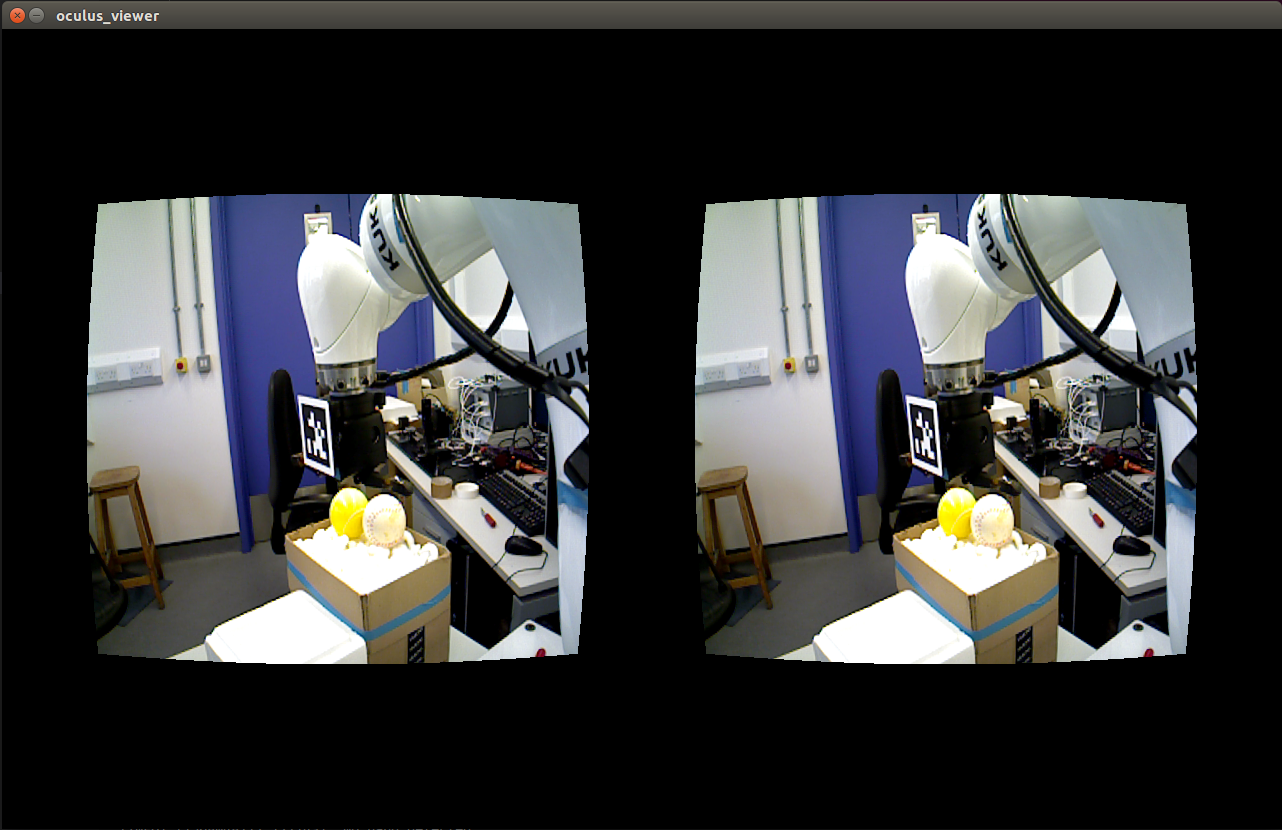
\includegraphics[width=14cm]{figures/oculus_view}
    \caption{Workspace as viewed inside the Oculus}
    \label{fig:oculus_view}
\end{figure}


\section{Visual Fiducial}

Seeing that the long-term goal of this project is to investigate autonomous robotic grasping a reference between the \gls{rgbd} camera and the robot must be established. A first attempt at this is done using an AprilTag fiducial on a 3D printed marker panel. The camera recognises a predefined AprilTag of known size and calculates its position and orientation from the camera intrinsics. Whether this is sufficiently accurate for the purposes of autonomous robotic grasping still needs to be investigated. Note that the AprilTag does not always need to be visible if the calibration is done before starting the task. This is due to the fact that the transform from KUKA base to camera does not change as both the camera and the KUKA are static in this scenario. Also note how in Figure \ref{fig:camera_frames_rviz} the \texttt{tag\_frame} exist in the tree but is currently not displayed.

\begin{lstlisting}[language=bash, caption={Launching camera AprilTag node}]
roslaunch vision camera_apriltag.launch
\end{lstlisting}

\begin{figure}[h]
    \centering
    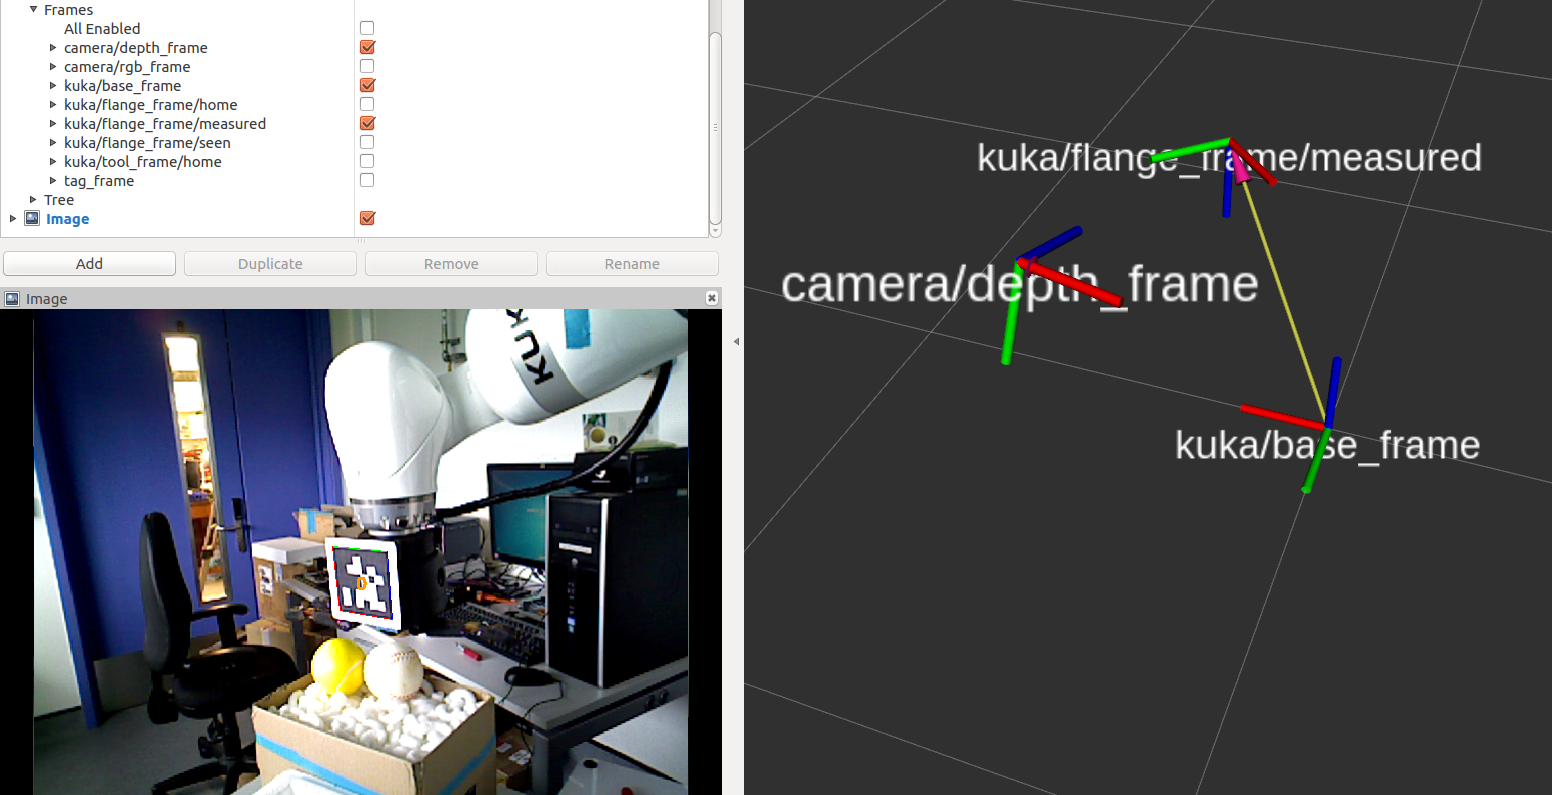
\includegraphics[width=\textwidth]{figures/camera_frames_rviz}
    \caption{Camera pose calculation in KUKA base frame}
    \label{fig:camera_frames_rviz}
\end{figure}

\newpage

"AprilTag is a visual fiducial system, useful for a wide variety of tasks including augmented reality, robotics, and camera calibration. Targets can be created from an ordinary printer, and the AprilTag detection software computes the precise 3D position, orientation, and identity of the tags relative to the camera. The AprilTag library is implemented in C with no external dependencies. It is designed to be easily included in other applications, as well as be portable to embedded devices. Real-time performance can be achieved even on cell-phone grade processors. The fiducial design and coding system are based on a near-optimal lexicographic coding system, and the detection software is robust to lighting conditions and view angle." \cite{AprilTag}

\begin{figure}[h]
    \centering
    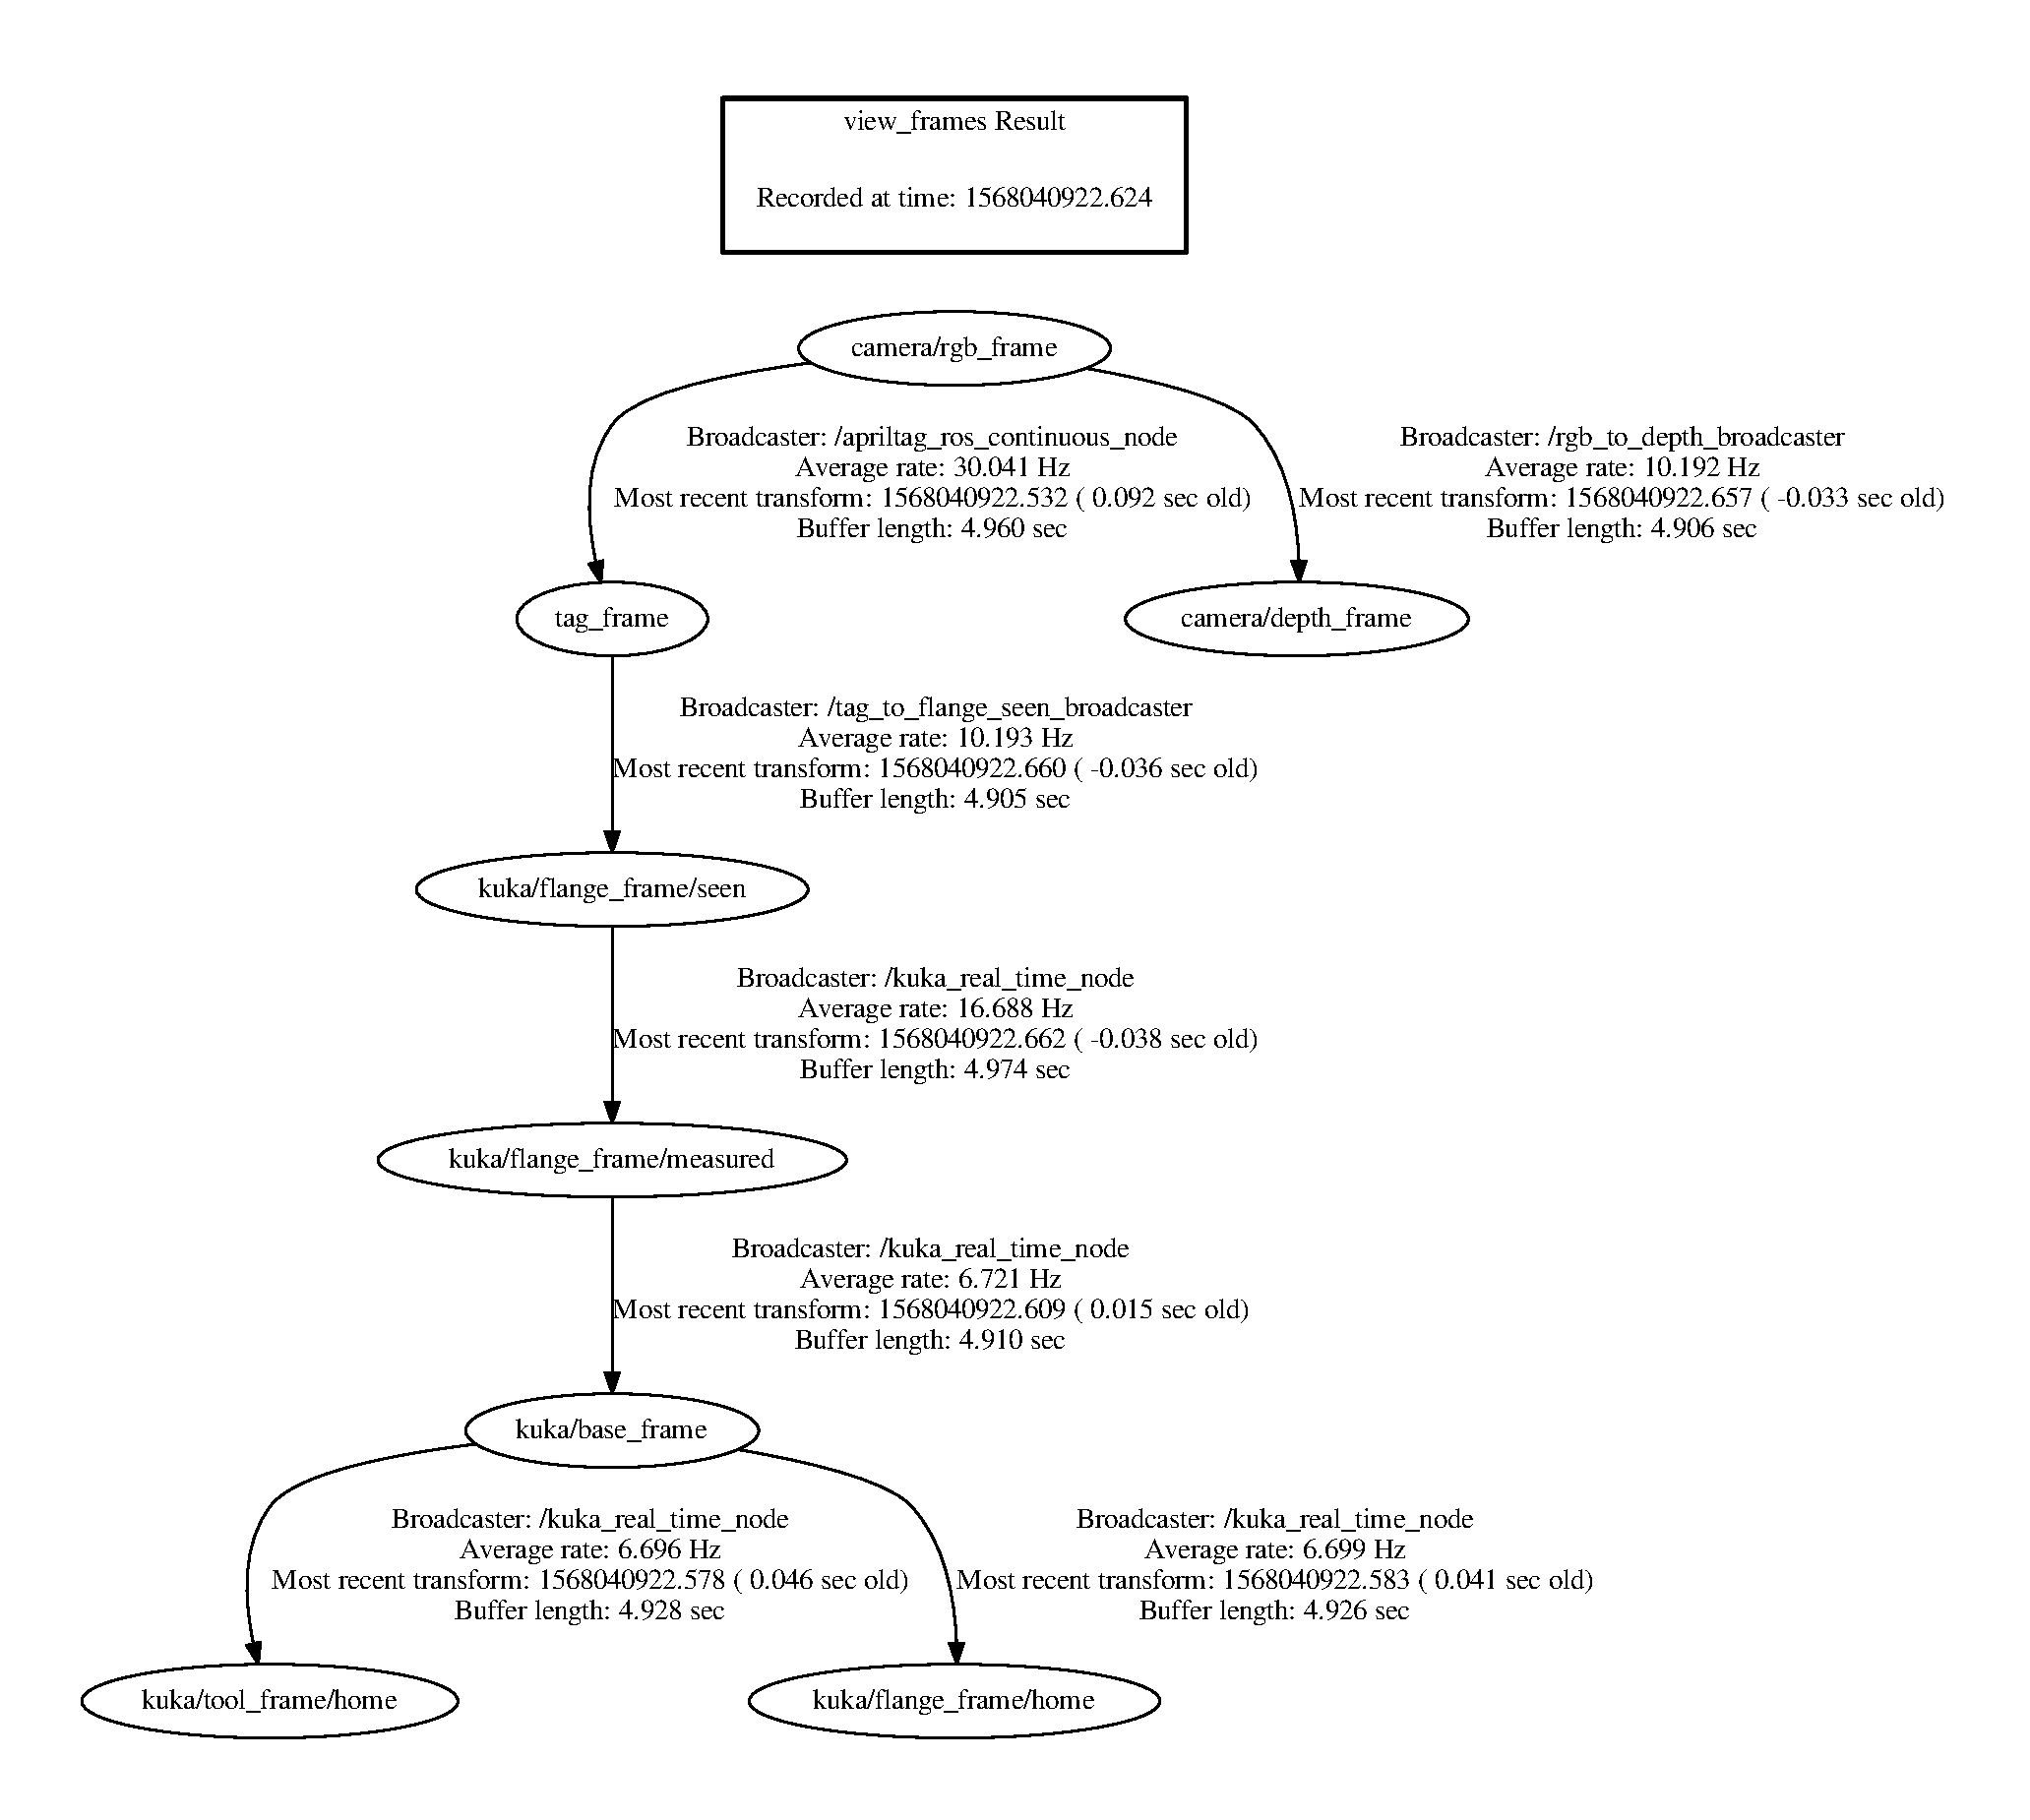
\includegraphics[width=\textwidth]{figures/camera_frames}
    \caption{Tf tree when camera\_apriltag and a KUKA control node running}
    \label{fig:camera_frames}
\end{figure}

\newpage
\section{RGB-D Fusion}\label{rgbd}

To merge the camera's RGB data with its depth data a launch file was set up in the \texttt{vision} folder. It uses the \texttt{image\_pipeline} module. To launch the \gls{rgbd} fusion type in the following. A preconfigured RViz window opens (see Figure \ref{fig:rviz}) to inspect the fused data. 

\begin{lstlisting}[language=bash, caption={Launching \gls{rgbd} fusion nodes}]
roslaunch vision register_rgbd.launch
\end{lstlisting}

\begin{figure}[h]
    \centering
    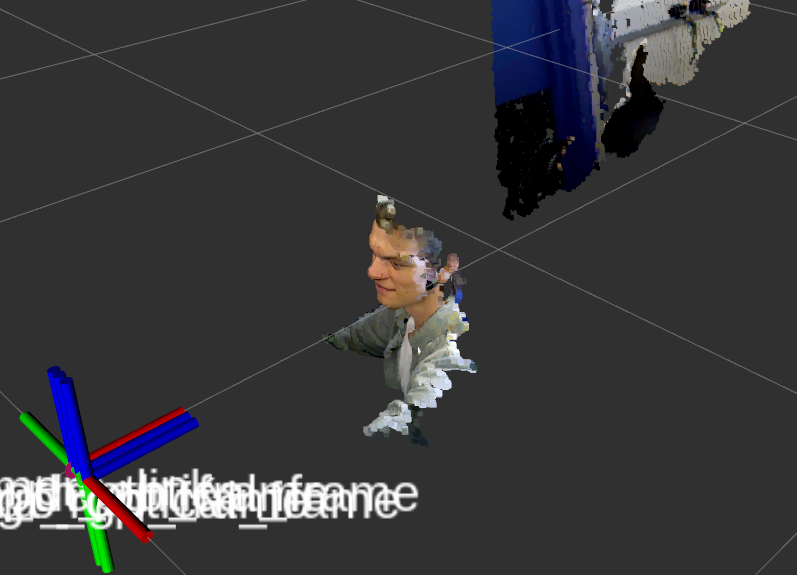
\includegraphics[width=8cm]{figures/rgbd_fusion}
    \caption{RViz showing fused \gls{rgbd} data}
    \label{fig:rviz}
\end{figure}

For autonomous grasping prediction using depth data (see chapter \ref{grasping}) a reference between the KUKA base frame and the camera depth frame must be established. The approach used for this estimation in this project currently is determining the cameras RGB optical frame using the AprilTag library and then rigidly transforming to the depth optical frame of the camera. The merged \gls{rgbd} data produced by this launch file could be used to get a more accurate estimate of the tag transform relative to the camera depth frame. This might be a sensible approach:

\begin{enumerate}
	\item Detect AprilTag using RGB camera  
	\item Get RGB pixels that correspond to the marker panel
	\item Fuse with depth pixels
	\item Reconstruct the transform from AprilTag to depth frame directly from landmarks (e.g. translation is depth pixel's value of tag's center and orientation could be calculated by constructing a plane that intersects all four corners of tag)
\end{enumerate} 

It is worth investigating if higher accuracies can be achieved for the estimation of the depth frame using this approach compared to the current one (see chapter \ref{future}). 

\chapter{Autonomous Grasping}\label{grasping}

This is a first attempt at investigating autonomous grasping using a \gls{rgbd} camera and neural networks to process depth images. The proposed research question is whether the performance of existing neural networks (such as presented in \cite{Grasping}) can be enhanced by a human in the loop. Since an intuitive user interface for the KUKA robot and robotic hand has been developed in this project it should be investigated whether performance scores can be improved using data that was generated from the systems presented earlier in this report. 

As a first step the pretrained neural network presented in \cite{Grasping} is used to get a first impression of the accuracy of their system and potential areas of improvement. See the network architecture of their so called generative grasping convolutional neural network (GGCNN) in Figure \ref{fig:arch}. Start the code for grasping prediction with the terminal commands below. In the image viewer select the desired prediction topic (e.g. \texttt{ggcnn/img/grasp}).

\begin{figure}[h]
    \centering
    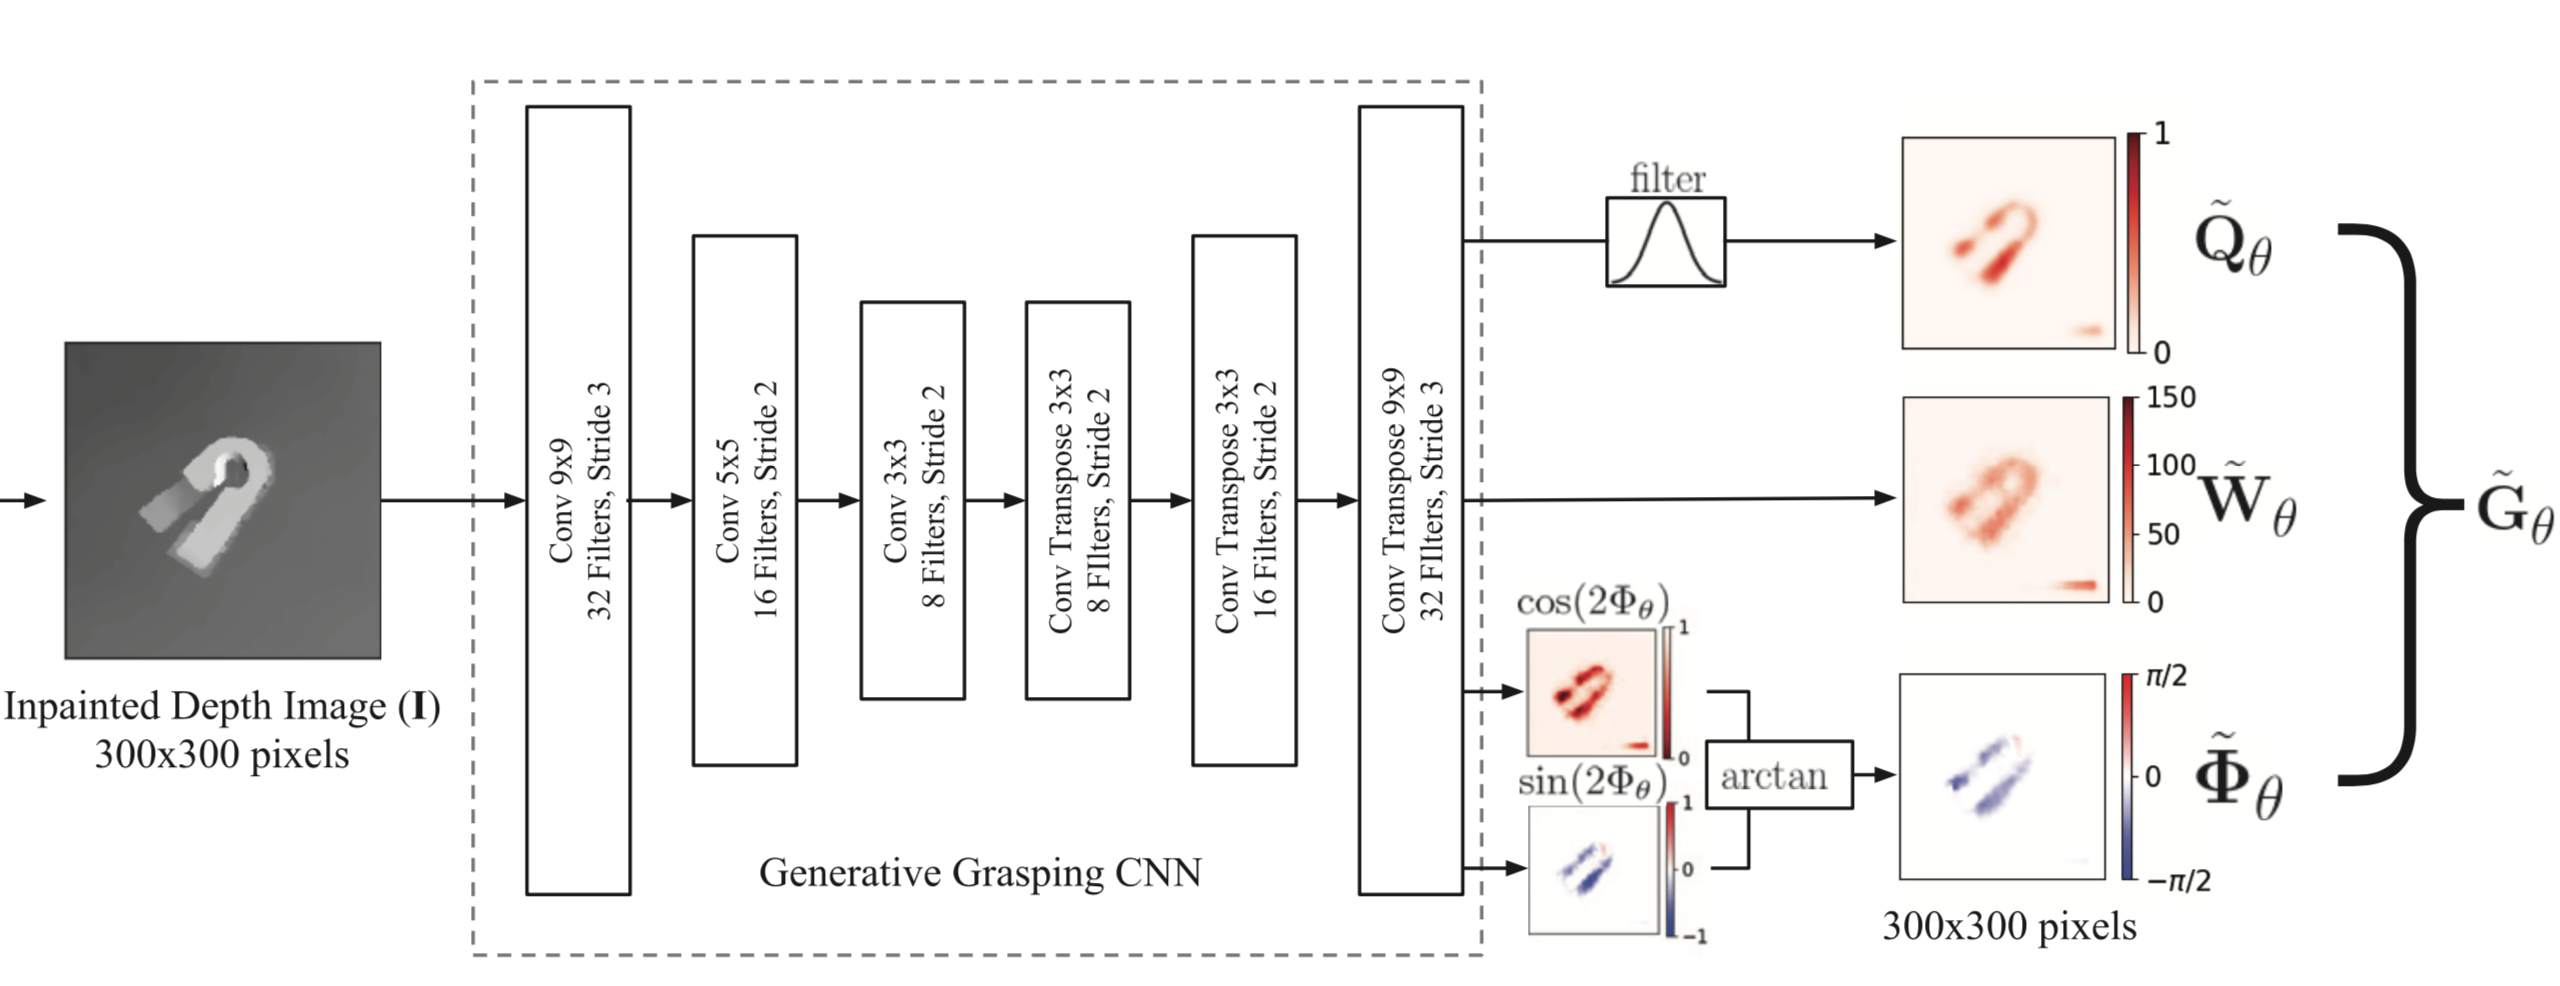
\includegraphics[width=15cm]{images/arch}
    \caption{Network architecture of GGCNN \cite{Grasping}}
    \label{fig:arch}
\end{figure}

\begin{lstlisting}[language=bash, caption={Launching grasp prediction node}]
# in a terminal type
roslaunch grasping grasping.launch
# in a new terminal type
conda activate grasping_py27 && rosrun grasping ggcnn.py
# when done 
conda deactivate
\end{lstlisting}

\newpage
\begin{figure} [h]
\centering
\begin{minipage}{.4\textwidth}
  \centering
  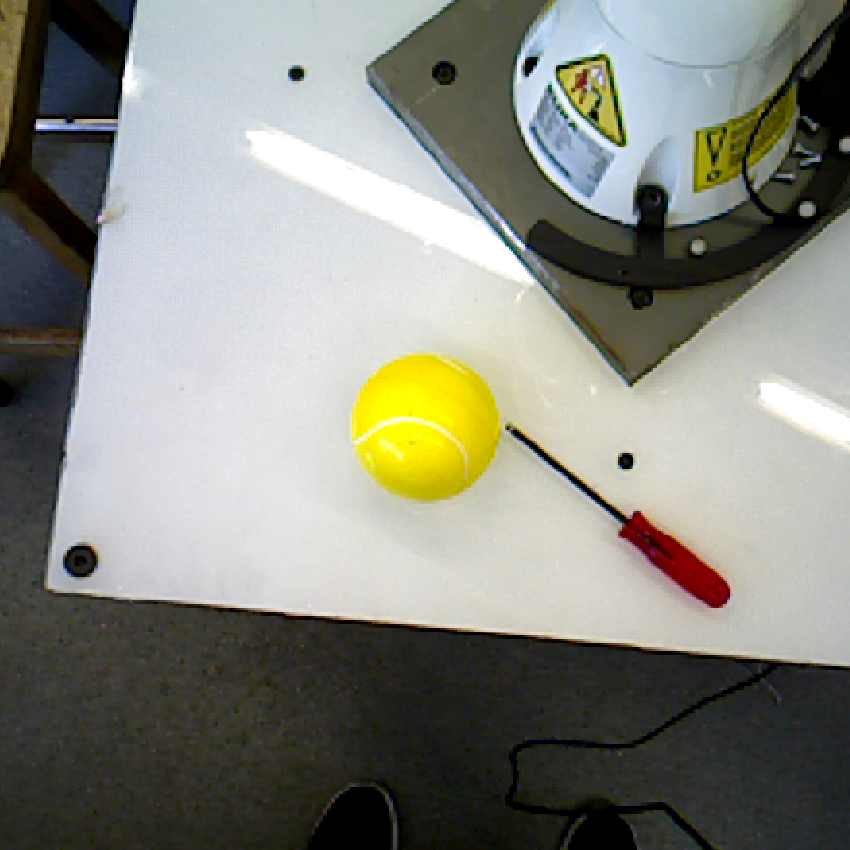
\includegraphics[height=6cm]{figures/pred_ball_rgb}
  \captionof{figure}{RGB view}
\end{minipage}
\begin{minipage}{.4\textwidth}
  \centering
  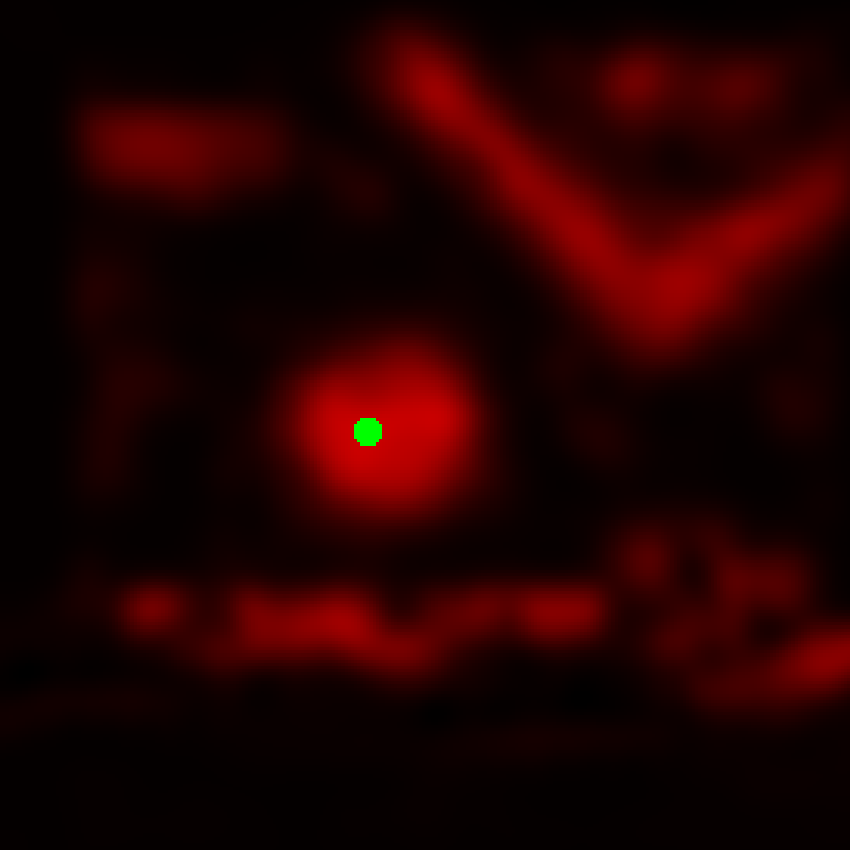
\includegraphics[height=6cm]{figures/pred_ball}
  \captionof{figure}{Grasping point prediction}
  \label{img:ball_pred}
\end{minipage}
\end{figure}

\begin{figure} [h]
\centering
\begin{minipage}{.4\textwidth}
  \centering
  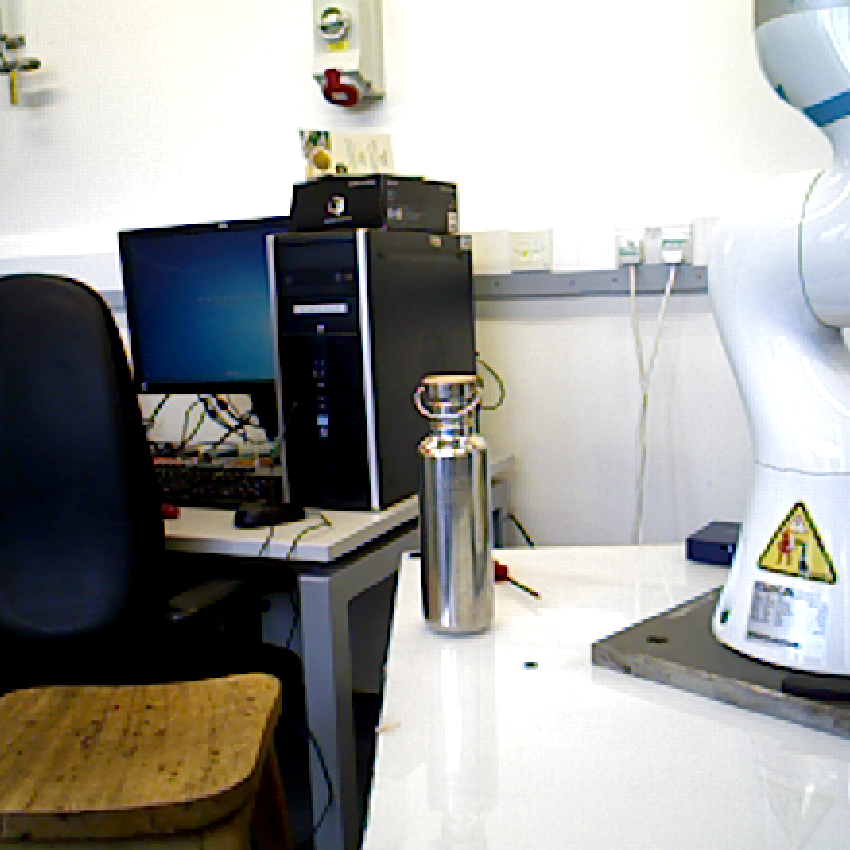
\includegraphics[height=6cm]{figures/pred_bottle_rgb}
  \captionof{figure}{RGB view}
\end{minipage}
\begin{minipage}{.4\textwidth}
  \centering
  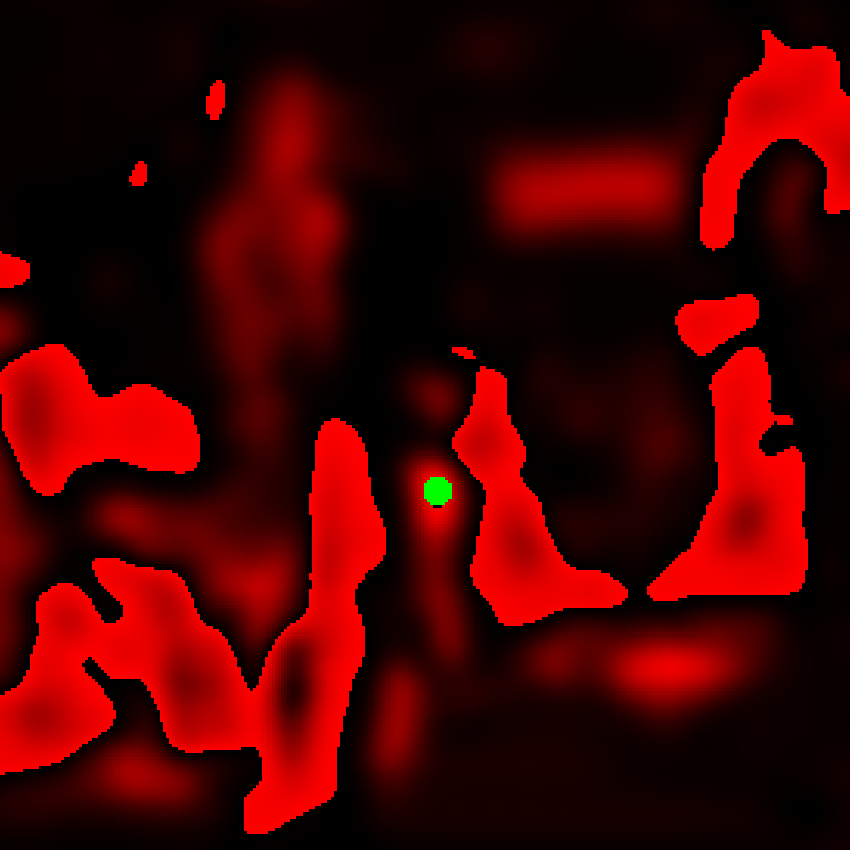
\includegraphics[height=6cm]{figures/pred_bottle}
  \captionof{figure}{Grasping point prediction}
  \label{img:bottle_pred}
\end{minipage}
\end{figure}

The \texttt{TransformStamped} of the predicted grasping pose is also published (however with a fixed rotation). It still needs to be investigated how to best estimate the tool orientation from the neural network output (see chapter \ref{future}). To see how Morrison et al. work with the predicted data and achieve closed loop control of grasping movements, it is recommended to check the code in the "GGCNN Kinova Grasping" GitHub repository.

Since the neural network's predictions are not very stable a post-processing filtering step should be considered. An additional neural network which is appended to the existing one (Figure \ref{fig:arch}) could serve this purpose. It is most sensible to work with the whole grasping "heat map" that is produced by the first neural network (as opposed to just the final prediction) to not loose any valuable abstraction the GGCNN makes. A second network could then use this preprocessed data and predict the full transformation from camera depth frame to the grasping target. This transform can then be transferred into the KUKA reference frame with a relation that has been established with Hand-Eye calibration using the AprilTag fiducial.

Training the second neural network could be done using data that was collected using the Leap Motion KUKA node. A dataset of possible grasping poses could be recorded from desired tool transform which is continuously published by the Leap Motion KUKA node. If this is sampled at a high frequency and paired with the corresponding GGCNN prediction a dataset for training of the second network could be build up. The workflow for dataset collection could look like this. 

\begin{enumerate}
	\item Determine transform from KUKA base to camera depth frame
	\item Choose one item to grasp (e.g. cup)
	\item Place object in workspace and keep robot in home position
	\item Keep camera on tripod and start GGCNN
	\item Collect 1000 predicted heat maps of workspace (approx. 1 minute at 15 Hz prediction rate)
	\item Use Leap KUKA node to generate 1000 possible grasping tool transforms (approx. 30 seconds at 30 Hz sampling rate)
	\item Choose other objects and repeat steps 2 to 6
	\item Train appended neural network with collected data
\end{enumerate}

\begin{figure}[h]
    \centering
    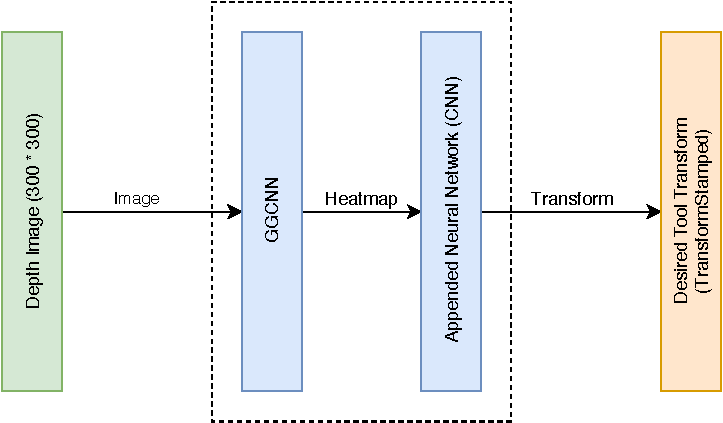
\includegraphics[width=12cm]{images/architecture}
    \caption{Enhanced GGCNN Overview}
    \label{fig:architecture}
\end{figure}

\chapter{Future Work}\label{future}

Some ideas on future work: 
\begin{enumerate}
	\item Bug fix: if time-out is set very long and no new tool transforms are published to the KUKA control node, the robot stays in the last position which it successfully received. Once new information is published on the topic the robot tries to move there immediately using a real time motion. This may cause problems when the jump is too big (hence we should rather do a PTP movement if the jump is larger than a threshold). For now either leave the default time-out and the robot will move safely to its home position once the signal is lost or be sure to publish a pose which is close to the one where you left off.
	\item Evaluate accuracy of AprilTag tracking using RGB optics. Is it sufficient for autonomous grasping? 
	\item Calculate transform from depth optical frame to tag using approach in section \ref{rgbd} and compare accuracy with RGB optics approach. 
	\item Control two robots using one Leap Motion. Only thing that needs to be changed is that two interaction boxes need to be formed and both hands need to be processed (not only hand which is visible the longest).
	\item Further investigation of autonomous robotic grasping. Test the proposed approach to improve GGCNN using a human in the loop. 
	\item Integration of force detection in robotic hand node. Limit grasping once pressure threshold reached.
	\item Depending on \gls{kst} advancement, publish KUKA status in real-time mode. The \gls{kst} currently only supports reliable status information (i.e. "getters") in \gls{ptp} mode and not during direct servoing.
	\item Make more complex tool transforms possible (full (4,4) transformation matrix in configuration file) and calculate home pose accordingly.
	\item Determine virtual Leap Motion transform relative to tool home transform and not KUKA base frame. Advantage is that this will adjust the virtual Leap Motion position if a custom home pose is given in the configuration file. This would make the system even more modular (e.g. for KUKA robots that are mounted on the ceiling or the wall).
	\item Visualise interaction box, give users feedback if they are holding their hand in a valid starting position and orientation.
	\item Use calibrated DH parameters. The DH parameters used by the \gls{kst} can be changed in the function \texttt{constDhDataOf7R800.m} of the KUKA Sunrise Toolbox.
\end{enumerate}

\printbibliography

\end{document}